% Stanford University PhD thesis style -- modifications to the report style
% This is unofficial so you should always double check against the
% Registrar's office rules
% See http://library.stanford.edu/research/bibliography-management/latex-and-bibtex
%
% Example of use below
% See the suthesis-2e.sty file for documentation
%
\documentclass[12pt]{report}
\usepackage[online]{suthesis-2e}
\usepackage{dblfloatfix}
\usepackage{graphicx}
\usepackage{todonotes}
\usepackage{floatrow}


%% This turns references into clickable hyperlinks.
\usepackage[bookmarks,backref=true,linkcolor=blue]{hyperref} %,colorlinks
\hypersetup{
  pdfauthor = {},
  pdftitle = {},
  pdfsubject = {},
  pdfkeywords = {},
  colorlinks=false,
  linkcolor= blue,
  citecolor= blue,
  pageanchor=true,
  urlcolor = blue,
  plainpages = false,
  linktocpage
}

% each of the following has two versions
%   \crefname{environmentname}{singular}{plural}, to be used mid-sentence
%   \Crefname{environmentname}{singular}{plural}, to be used at the beginning of a sentence
\usepackage{cleveref}

\crefname{chapter}{Chapter}{Chapter}
\crefname{table}{Table}{Tables}
\Crefname{table}{Table}{Tables}
\crefname{figure}{Fig.}{Figs.}
\Crefname{figure}{Figure}{Figures}

\dept{Computer Science}

%%%%%%%%%%%%%%%%%%%%%%%%%%%%%%%%%%%%%%%%%%%%%%%%%%%%%%%%%%%%%%%%%%%%%
% make complete reference clickable
\newcommand{\figref}[1]{\hyperref[#1]{Fig.~\ref*{#1}}}
\newcommand{\secref}[1]{\hyperref[#1]{\S\ref*{#1}}}
\newcommand{\tabref}[1]{\hyperref[#1]{Table~\ref*{#1}}}
\newcommand{\defref}[1]{\hyperref[#1]{Definition~\ref*{#1}}}
\newcommand{\equref}[1]{\hyperref[#1]{Eq.~\ref*{#1}}}
\newcommand{\lstref}[1]{\hyperref[#1]{Listing~\ref*{#1}}}

\begin{document}
\title{Declarative Interaction Design\\for Data Visualization}
\author{Arvind Satyanarayan}
\principaladviser{Jeffrey Heer}
\firstreader{Maneesh Agrawala}
\secondreader{James Landay}

\tablespagefalse

\beforepreface
\prefacesection{Abstract}
This thesis tells you all you need to know about...
\prefacesection{Acknowledgments}
I would like to thank...
\afterpreface

% !TEX root = ./thesis.tex
\graphicspath{{./vega-lang/figures/}}
\chapter{Declarative Primitives for Interaction Design}
\label{sec:vg}

Reactive Vega builds on a long-running thread of research on declarative
visualization design, popularized by the Grammar of
Graphics~\cite{wilkinson:grammar} and Polaris~\cite{stolte:polaris} (now
Tableau).

Visual encodings are defined by composing graphical primitives called
\emph{marks}~\cite{bostock:protovis}, which include \emph{arcs}, \emph{areas},
\emph{bars}, \emph{lines}, plotting \emph{symbols} and \emph{text}. Marks are
associated with datasets, and their specifications map tuple values to visual
properties such as position and color. Scales and guides (i.e., axes and
legends) are provided as first-class primitives for mapping a domain of data
values to a range of visual properties. Special \emph{group} marks serve as
containers to express nested or small multiple displays. Child marks and scales
can inherit a group's data, or draw from independent datasets.

Although interaction is a crucial component of effective
visualization~\cite{liu:mentalmodels, pike:interactionscience}, existing
declarative visualization models, including widely used tools such as
D3~\cite{bostock:d3} and ggplot2~\cite{wickham:ggplot2}, do not offer composable
primitives for interaction design. Instead, if they support interaction, they do
so through either a palette of standard techniques~\cite{bostock:protovis,
bostock:d3} or \emph{imperative} event handling callbacks. While the former
restricts expressivity, the later undoes many of the benefits of declarative
design. In particular, users are forced to contend with interaction execution
details, such as interleaved events and coordinating external state, which can
be complex and error\--prone~\cite{cooper:embedding, edwards:coherent,
myers:callbacks}.

In response, Reactive Vega introduces a model for \emph{declarative} interaction
design.

\section{Interaction Language Design}
\label{sec:vg:primitives}

\vspace{-10pt}

Reactive Vega models low-level events as composable data streams from which
higher-level semantic \emph{signals} can be constructed. Signals feed
\emph{predicates} and \emph{scale inversions}, to generalize interactive
selections at the level of item geometry (pixels) into interactive queries over
the data domain. \emph{Production rules} then use these queries to manipulate
the visualization's appearance. To facilitate reuse and sharing, these
constructs can be encapsulated as named \emph{interactors}: standalone, purely
declarative specifications of interaction techniques.

\vspace{-10pt}

\subsection{Event Streams and Signals}
\label{sec:vg:events}

\vspace{-10pt}

Reactive Vega adapts the semantics of Event-Driven Functional Reactive
Programming~\cite{wan:efrp}. Low-level input events (e.g., mouse events) are
captured as time-varying \emph{data streams}, rather than event callbacks. This
abstraction reduces the burden of composing and sequencing
events\,---\,operations that would require several callbacks and some external
state under an imperative paradigm. To this end, we introduce a syntax for
specifying event streams (\cref{fig:vg:eventStreams}). While prior work has
formulated regex-based symbols for event selection~\cite{kin:proton++} we
believe our approach, by mimicking CSS selectors, will be more familiar to
designers.

\begin{figure}[b!]
  \centering
  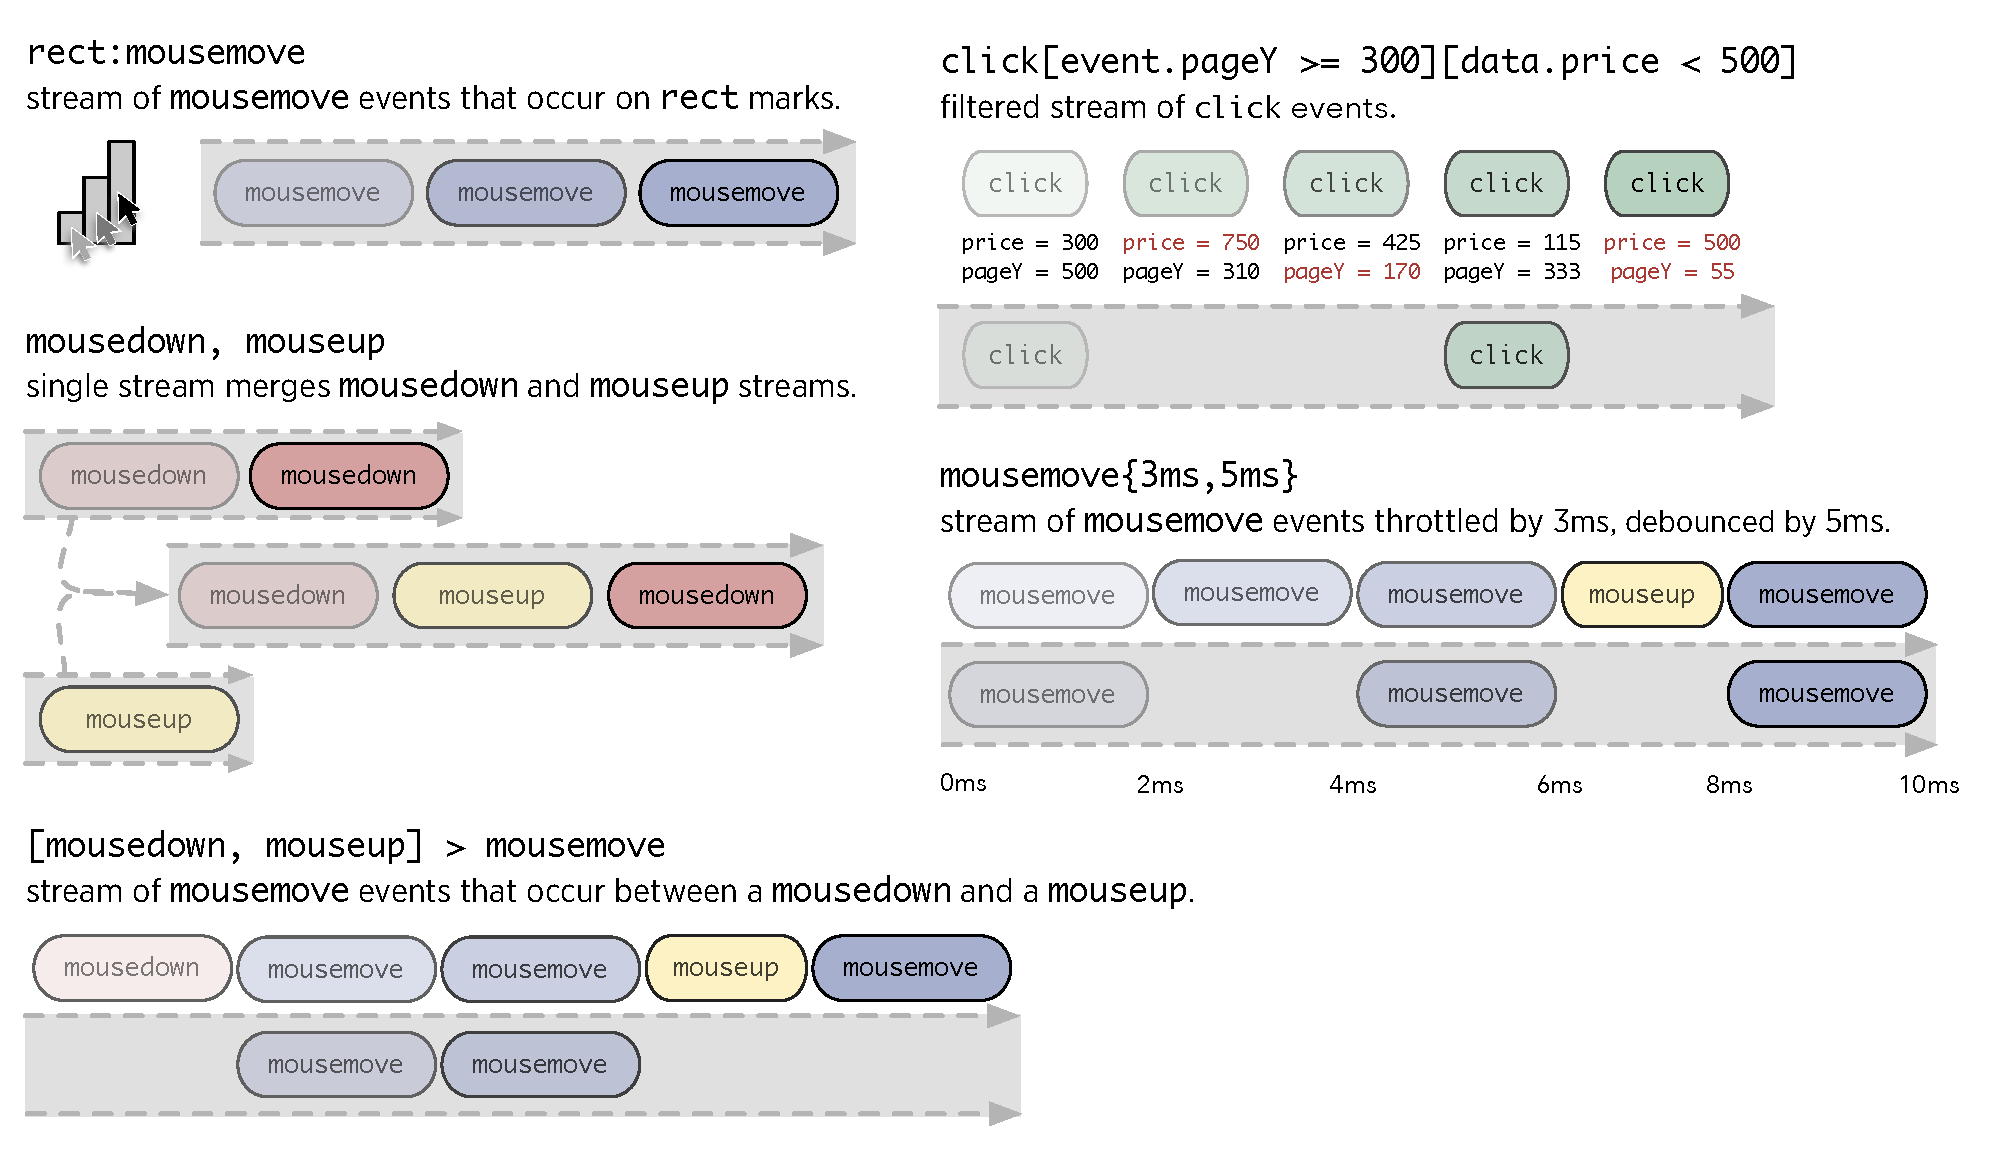
\includegraphics[width=\columnwidth]{eventStreams}
  \caption{Reactive Vega provides an event stream selector syntax, inspired by
  CSS selectors, to compose, filter, and sequence input events.}
  \label{fig:vg:eventStreams}
\end{figure}

A basic event stream selector is specified by a particular event type (e.g.,
\texttt{mousemove}), optionally prepended with the source of the
events\,---\,either a mark type (e.g., \texttt{rect:}) or name (e.g.,
\texttt{@cell:}). The comma operator (\texttt{,}) merges streams to produce a
single stream with interleaved events. Square brackets (\texttt{[]}) filter
events based on their properties. When followed by the right-combinator
(\texttt{>}), the brackets indicate a ``between filter,'' defining bounding
events for the stream. For instance, \texttt{[mousedown, mouseup] > mousemove}
captures \texttt{mousemove} events that occur between a \texttt{mousedown} and
\texttt{mouseup} (i.e., ``drag'' events). To throttle or debounce an event
stream, timing information can be specified between curly braces (e.g.,
\texttt{\{100, 200\}} throttles a stream by 100ms and debounces it by 200ms).
All operators are composable. For instance, \texttt{[mousedown[event.shiftKey],
window:mouseup] > window:mousemove\{100, 200\}} specifies a stream of throttled
and debounced drag events that are only triggered when the shift key is pressed.

With Reactive Vega, interaction events are a first-class data source. They can
be run through the full gamut of data transformations and can drive visual
encoding primitives. While doing so can usefully visualize a user's interaction,
for added expressivity, event streams can also be composed into reactive
expressions called \emph{signals}. By default, signals are evaluated using the
most recent event from a stream. However, signals can also define finite-state
machines by drawing from multiple streams\,---\,each stream triggers a state
transition.

Signals can be used to directly specify visual encoding primitives (e.g., a
mark's fill color) thereby endowing them with reactive semantics. When an event
fires, it enters appropriate streams and is propagated to corresponding signals;
signals are re-evaluated and dependent visual encodings re-rendered
automatically.

Upon definition, signals must be given unique names. These named entities are
then used to define the rest of an interaction technique, thereby decoupling
input events from downstream application logic. Thus, an interaction can be
triggered by a different set of events by simply rebinding signal declarations.
As we later demonstrate, rebinding is particularly useful for retargeting
interactions or for combining otherwise conflicting interactions.

\vspace{-10pt}

\subsection{Predicates and Scale Inversion}

\vspace{-10pt}

Selection is a fundamental operation in interactive visualization design~
\cite{heer:generalized}. Once a selection is made, subsequent operators can be
applied to manipulate the selected items. For visual design, it can be
sufficient to make a predetermined selection (e.g., ``select all rectangles'').
With interaction design, however, selections are driven by user
input\,---\,brushing over points of interest, or adjusting a slider to filter
data.

\begin{figure}[t!]
  \centering
  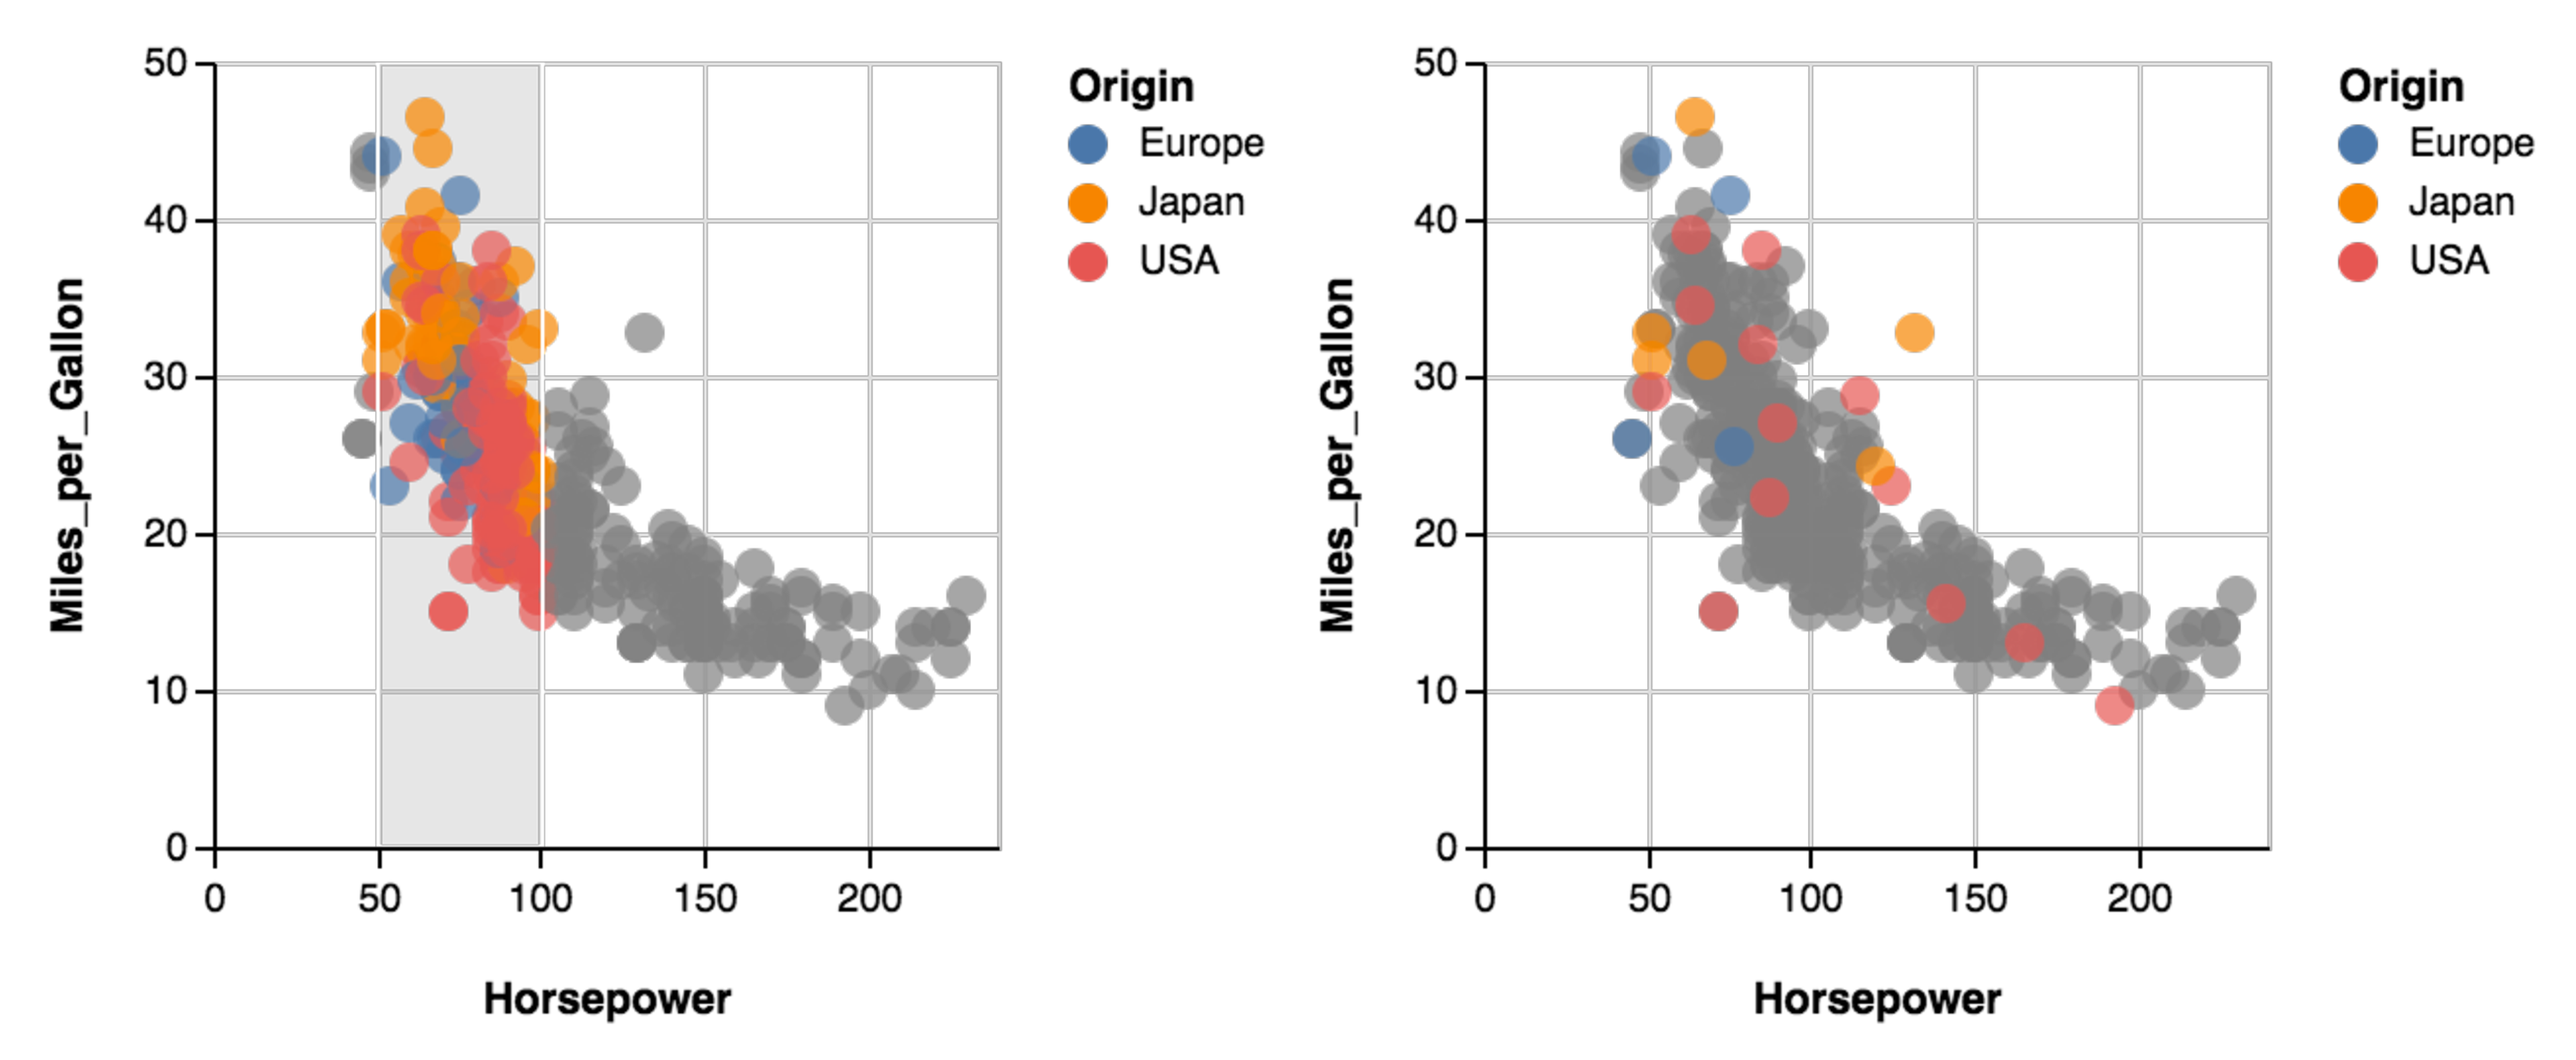
\includegraphics[width=0.9\columnwidth]{predicates}
  \caption{Points are highlighted using (left) an intensional predicate
  \texttt{50 $\leq$ Horsepower $\leq$ 100} or (right) an extensional predicate
  with members \texttt{\#56, \#110, \#79, \#95, \#40, \#120, ...}.}
  \label{fig:vg:predicates}
\end{figure}

To express interactive selections, we introduce reactive \emph{predicates}. As
shown in \cref{fig:vg:predicates}, predicates can be constructed either with an
\emph{intensional} definition\,---\,specifying conditions over properties of
selected members\,---\,or an \emph{extensional} one\,---\,explicitly enumerating
all members of a selection.

Predicate operands are typically signals and, as signals drawn from input event
streams, predicates express interactive selections at the visual (or pixel)
level by default. However, pixel-level selection is often insufficient. A single
visualization may have multiple distinct visual spaces, or an interactive
technique may wish to coordinate several visualizations. In such cases, it is
necessary to generalize an interactive selection into a query over the data
domain~\cite{heer:generalized}. Scale functions are a critical component in
visualization design~ \cite{wilkinson:grammar} as they transform data values
into visual values such as pixels or colors. By applying an \emph{inverted}
scale function to predicate operands, we can lift a predicate to the data
domain. \Cref{fig:vg:scaleInversion} demonstrates how a predicate defines an
interactive selection and, when coupled with scale inversions, an interactive
query to drive an overview\,+\,detail visualization.

\newpage
\begin{figure}[h!]
  \centering
  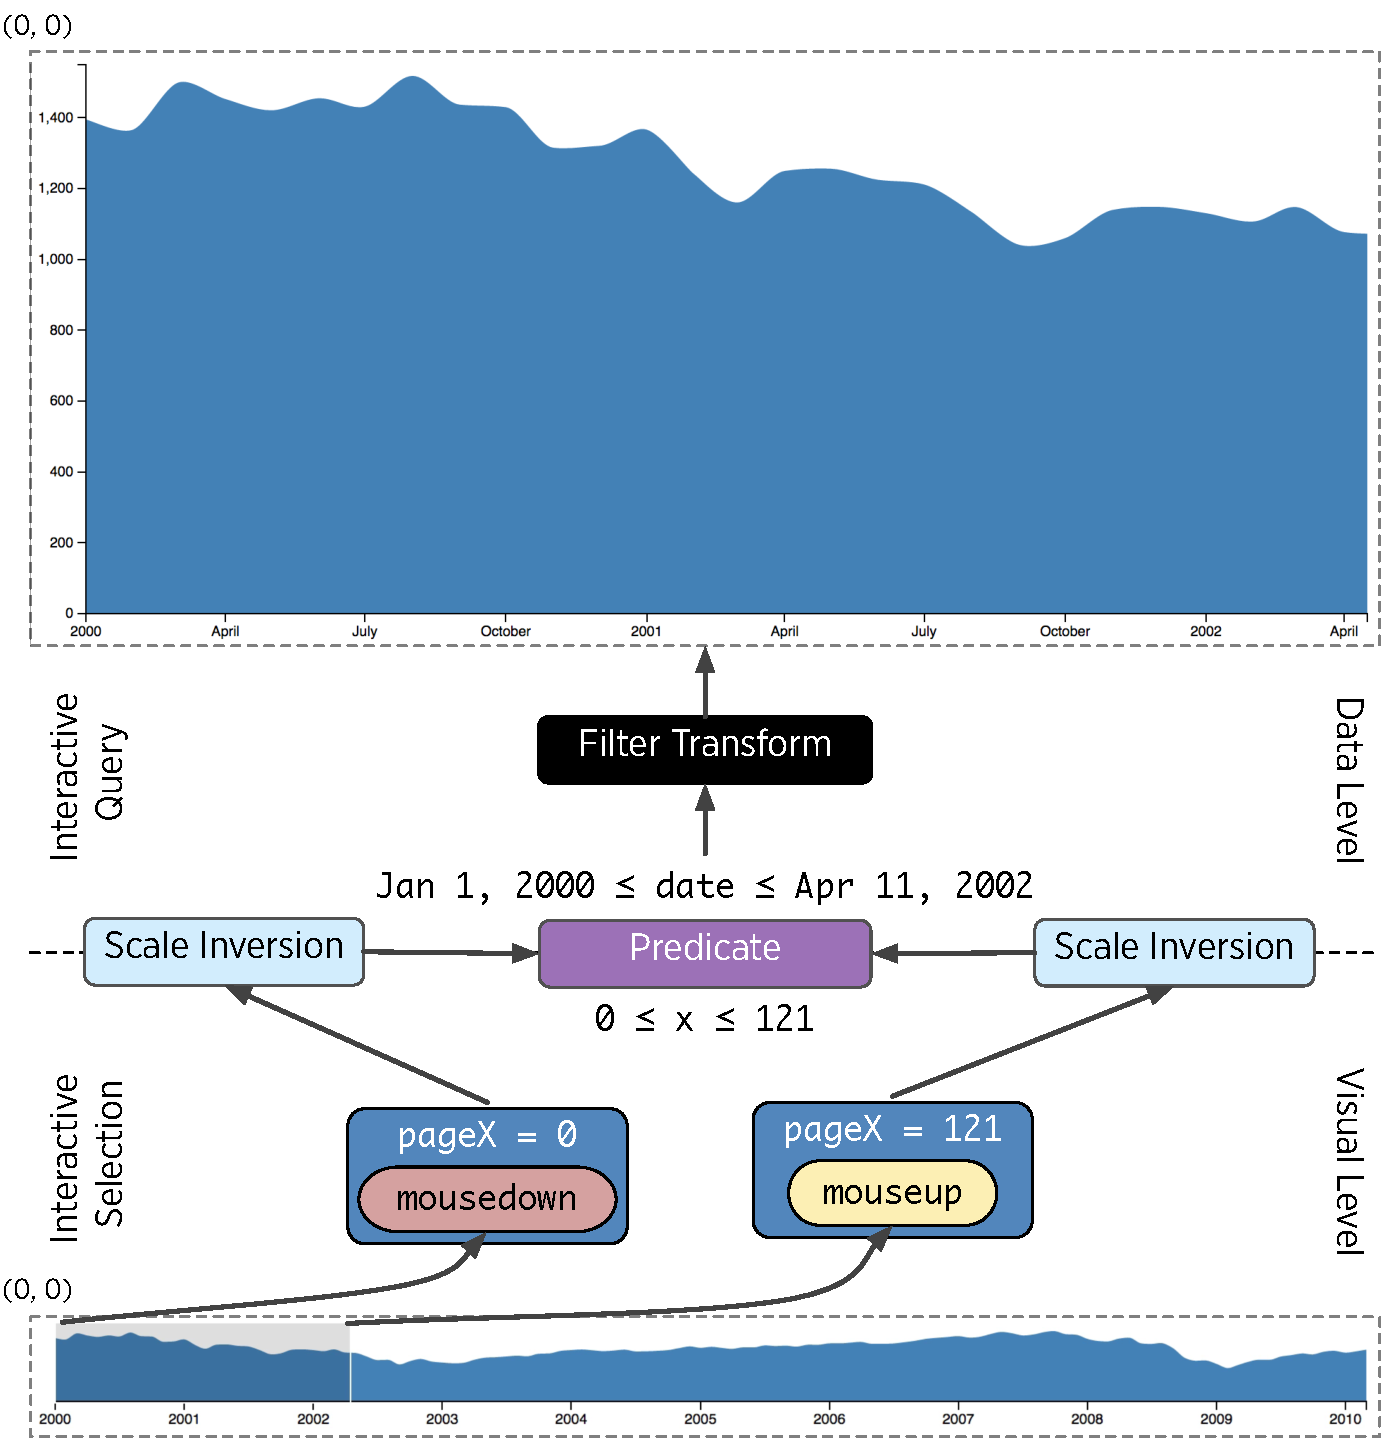
\includegraphics[width=\columnwidth]{scaleInversion}
  \caption{\emph{Predicates} use signal values to define interactive selections
of elements. Using \emph{scale inversions}, predicates can be generalized to
define interactive queries, and thus operate across different coordinate spaces:
overview (bottom) and detail (top).}
  \label{fig:vg:scaleInversion}
\end{figure}


\subsection{Production Rules}

\vspace{-10pt}

Production rules are an established design pattern for visualization
specification~\cite{heer:designpatterns} that we endow with reactive semantics.
A rule defines the outcome of evaluating an \texttt{if-then-else} chain to set
property values. For example, a rule might set a mark's fill color using
scale-transformed data if predicate \texttt{A} is true, set it to yellow is
predicate \texttt{B} is true, or otherwise set the color to grey by default.

\vspace{-10pt}

\subsection{User-Defined Functions}
\label{sec:udfs}

\vspace{-10pt}

During our design process, we encountered visualizations in which interactions
trigger custom data transforms. For example, sorting a co-occurrence matrix by
frequency or querying time-series data via relaxed
selections~\cite{holz:relaxed}. It is not feasible for a declarative language to
natively support all possible functions, yet custom operations must still be
expressible. Following the precedent of languages such as SQL, we provide
\emph{user-defined functions}. Such functions must be defined and registered
with the system at runtime, and can subsequently be invoked declaratively within
the specification. User-defined functions ensure that the language remains
concise and domain-specific, while ensuring extensibility to idiosyncratic
operations.

\vspace{-10pt}

\subsection{Encapsulated Interactors}

\vspace{-10pt}

To enable reuse of custom interaction techniques, Reactive Vega's interaction
primitives can be parameterized and encapsulated as named \emph{interactors}.
Inspired by Garnet's component of the same name~\cite{myers:garnet}, a Reactive
Vega's interactor can subsequently be applied to a visualization and functions
as a mixin. Its specification is merged into the host's and, to prevent
conflicts, its components are addressable only under its namespace.
\Cref{fig:vg:splomInteractor,fig:vg:brush} illustrate how a brushing
interaction (within a single scatterplot) can be extracted to a standalone
interactor, and reapplied to brush \& link a scatterplot matrix.
% !TEX root = ../thesis.tex
\section{Example Interactive Visualizations}
\label{sec:vg:examples}

\vspace{-10pt}

To evaluate the expressivity of our language, we present a range of examples and
demonstrate coverage over Yi~et~al.'s interaction
taxonomy~\cite{yi:understanding}. Yi~et~al. identify seven categories based on
user intent: \emph{select}, to mark items of interest; \emph{connect}, to show
related items; \emph{abstract/elaborate}, to show more or less detail;
\emph{explore}, to examine a different subset of data; \emph{reconfigure}, to
show a different arrangement of data; \emph{filter}, to show something
conditionally; and, \emph{encode}, to use a different visual encoding. It is
important to note that these categories are not mutually exclusive, and an
interaction technique can be classified under several categories. We choose
example interactive visualizations to demonstrate that our model can express
interactions across all seven categories and how, through composition of its
primitives, supports the accretive design of richer interactions.

\begin{figure}[h!]
  \centering
  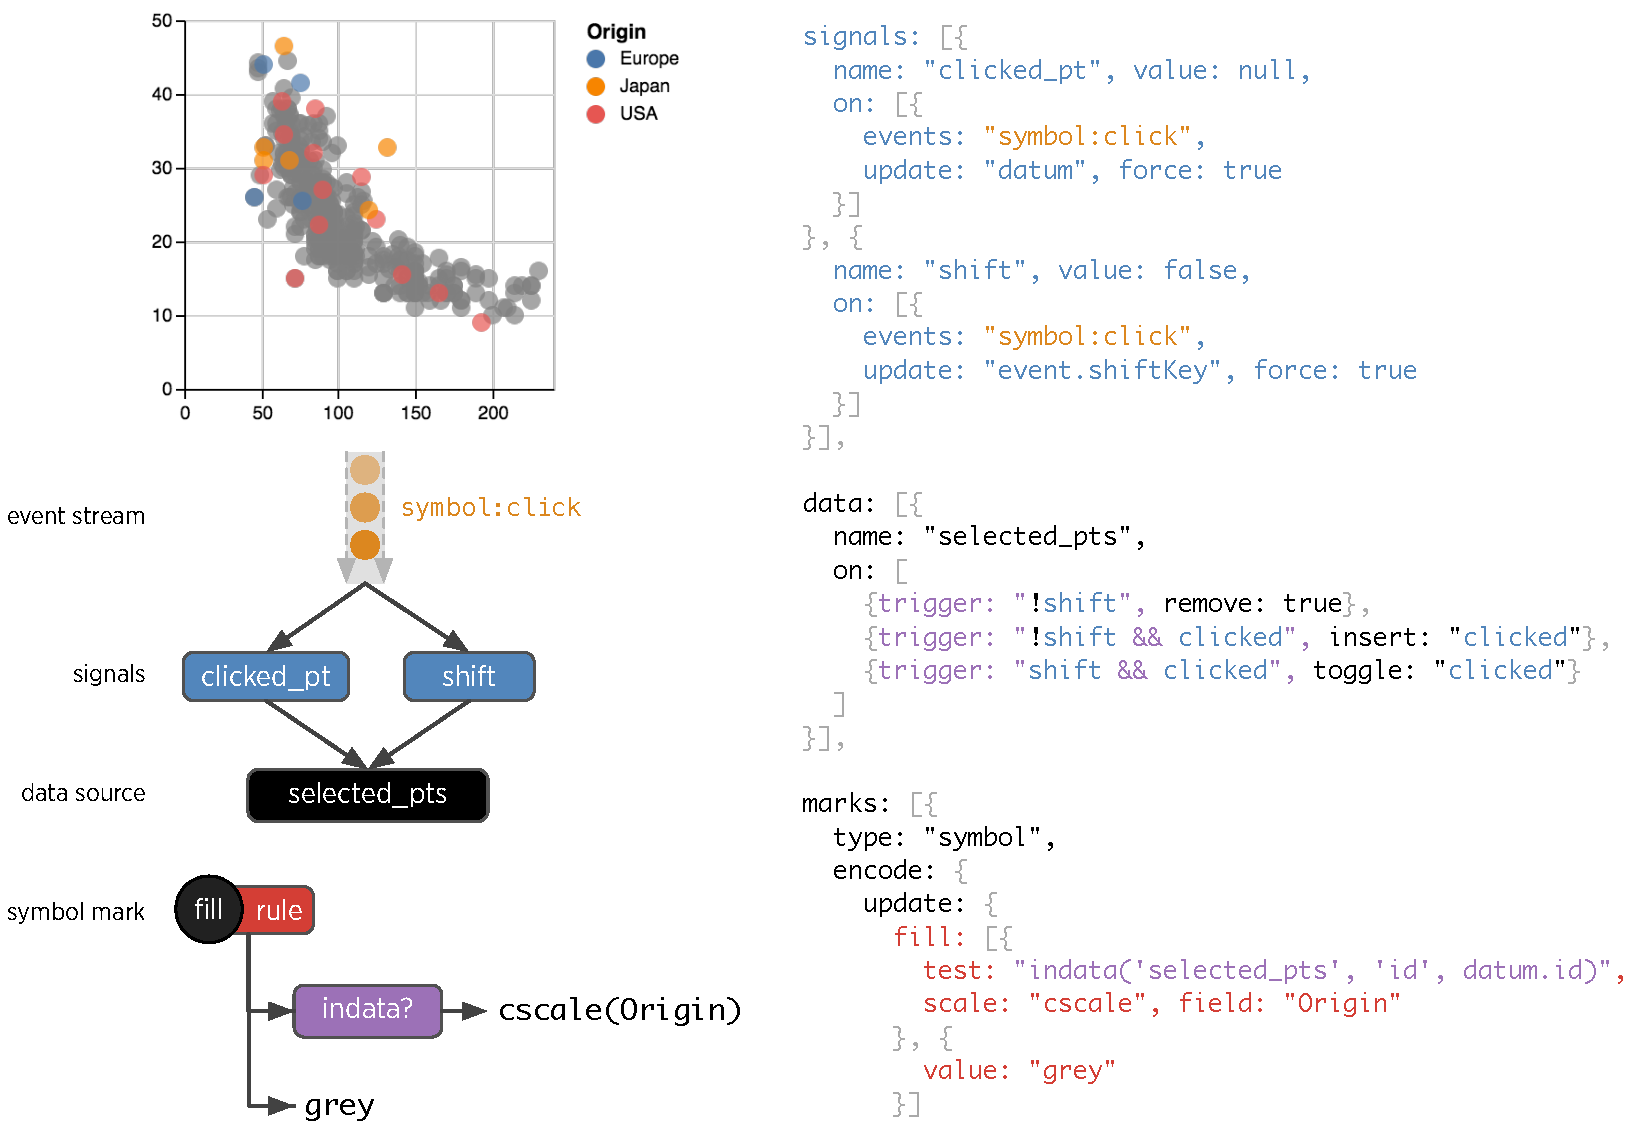
\includegraphics[width=\columnwidth]{shiftClick}
  \caption{Reactive Vega \textsc{json} for a click-to-highlight interaction.
  Signals over a click stream feed data transform to toggle values in a data
  source. A production rule uses a predicate to set marks' fill color.}
  \label{fig:vg:shiftClick}
\end{figure}

\subsection{Selection: Click/Shift-Click and Brushing}

\vspace{-7pt}

\Cref{fig:vg:shiftClick} provides a snippet of Reactive Vega \textsc{json} for a
click-to-highlight interaction. Signals constructed over a click stream feed
data transforms that toggle values in the \texttt{selected\_pts} data source. An
intensional predicate tests for the shift key. If it is not pressed, the data
source is cleared prior to inserting the clicked values. A production rule sets
the fill color of selected points using an extensional predicate.

Similarly, \cref{fig:vg:brush} demonstrates the Reactive Vega \textsc{json}
necessary to enable brush selections. Signals are registered to capture the
start and end positions of the brush, by default \texttt{mousedown} and
\texttt{[mousedown, mouseup] > mousemove}, respectively. Scale inversions are
invoked to calculate the data extents of the brush, which are used to define an
intensional predicate to express the brushed data range. As before, the
predicate is used within a production rule to set the fill color of selected
points.

\begin{figure}[h!]
  \centering
  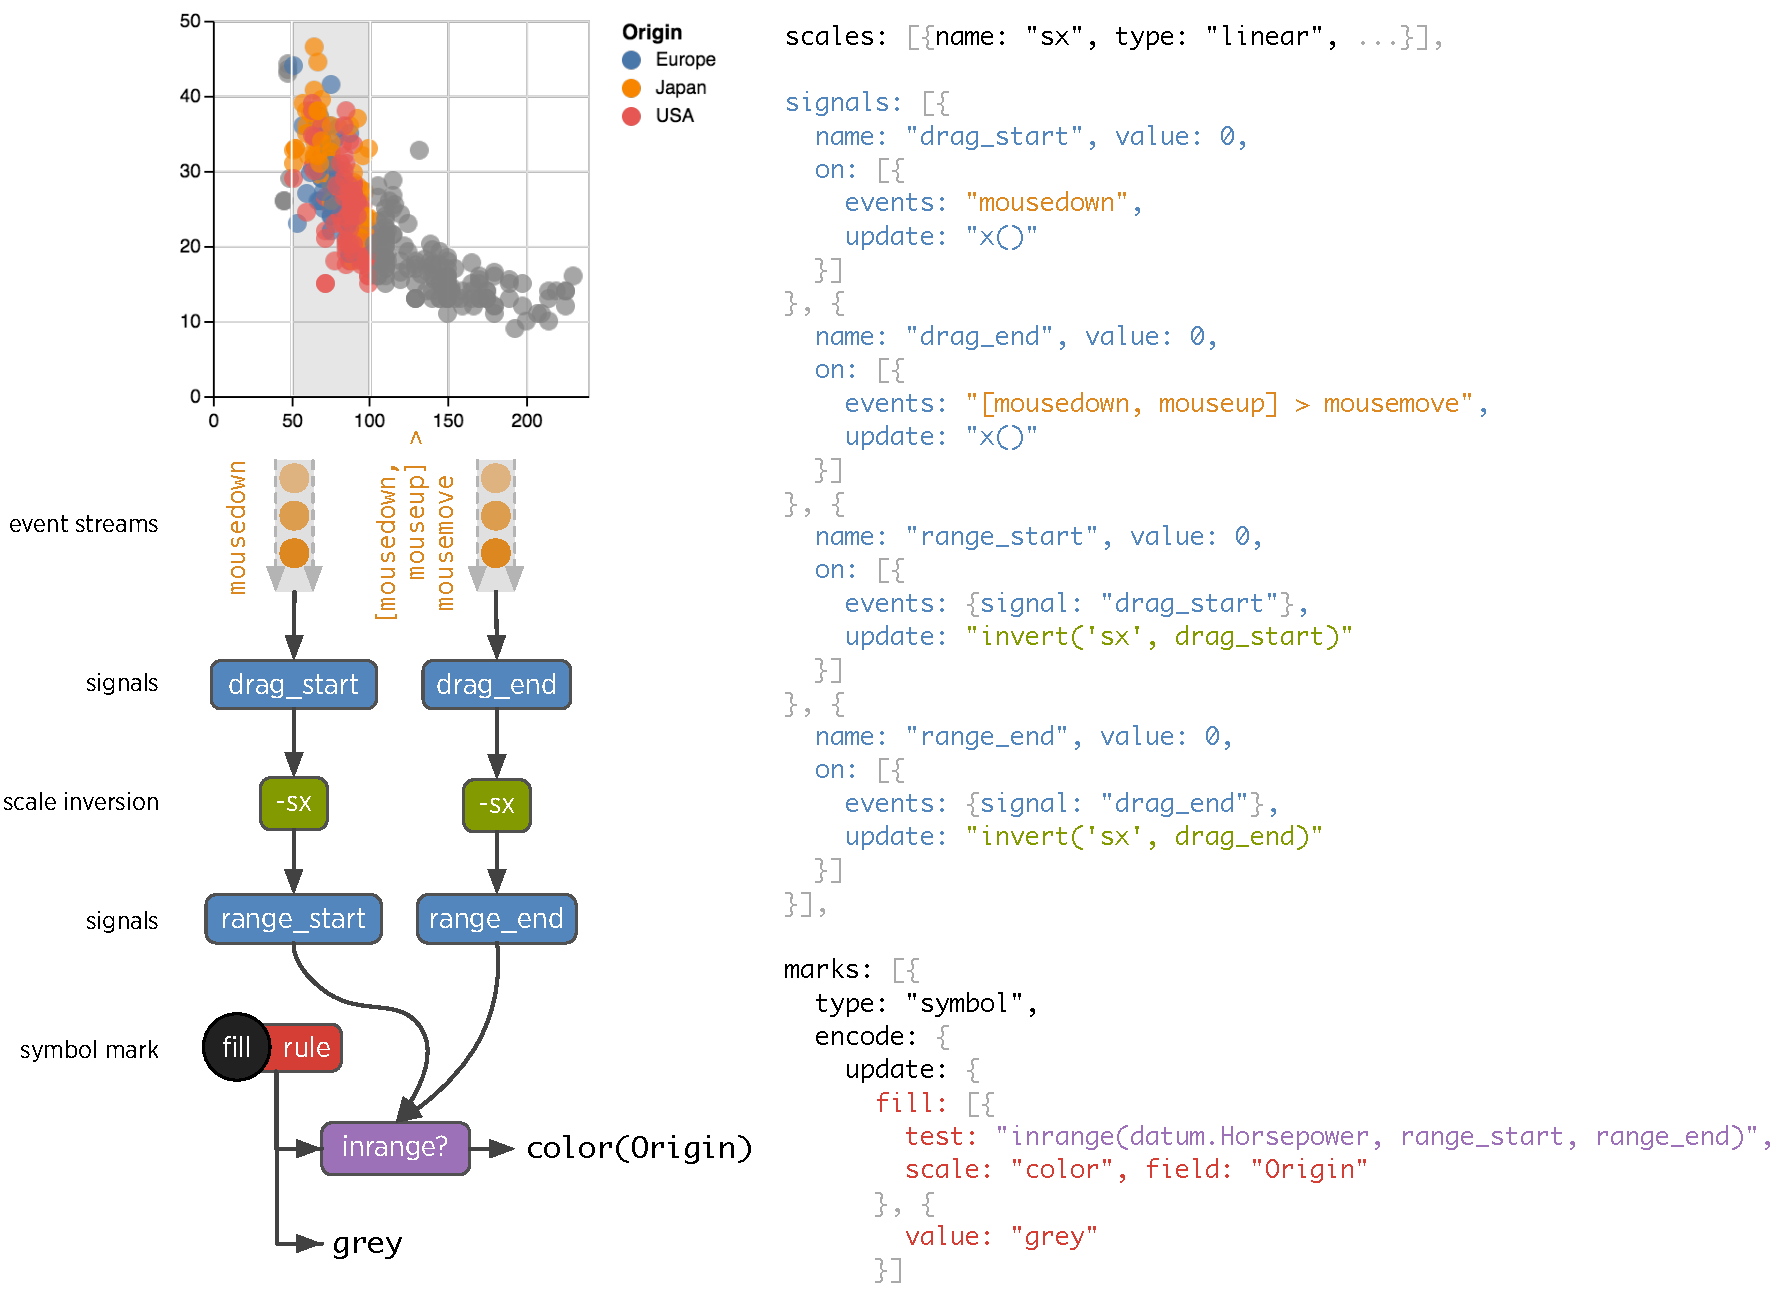
\includegraphics[width=0.91\columnwidth]{brush}
  \caption{A \textsc{json} snippet for one-dimensional brushing. Signals over
  drag events are inverted through the x-scale to construct a data query over
  the \texttt{Horsepower} field.}
  \label{fig:vg:brush}
\end{figure}

\begin{figure}[h!]
  \centering
  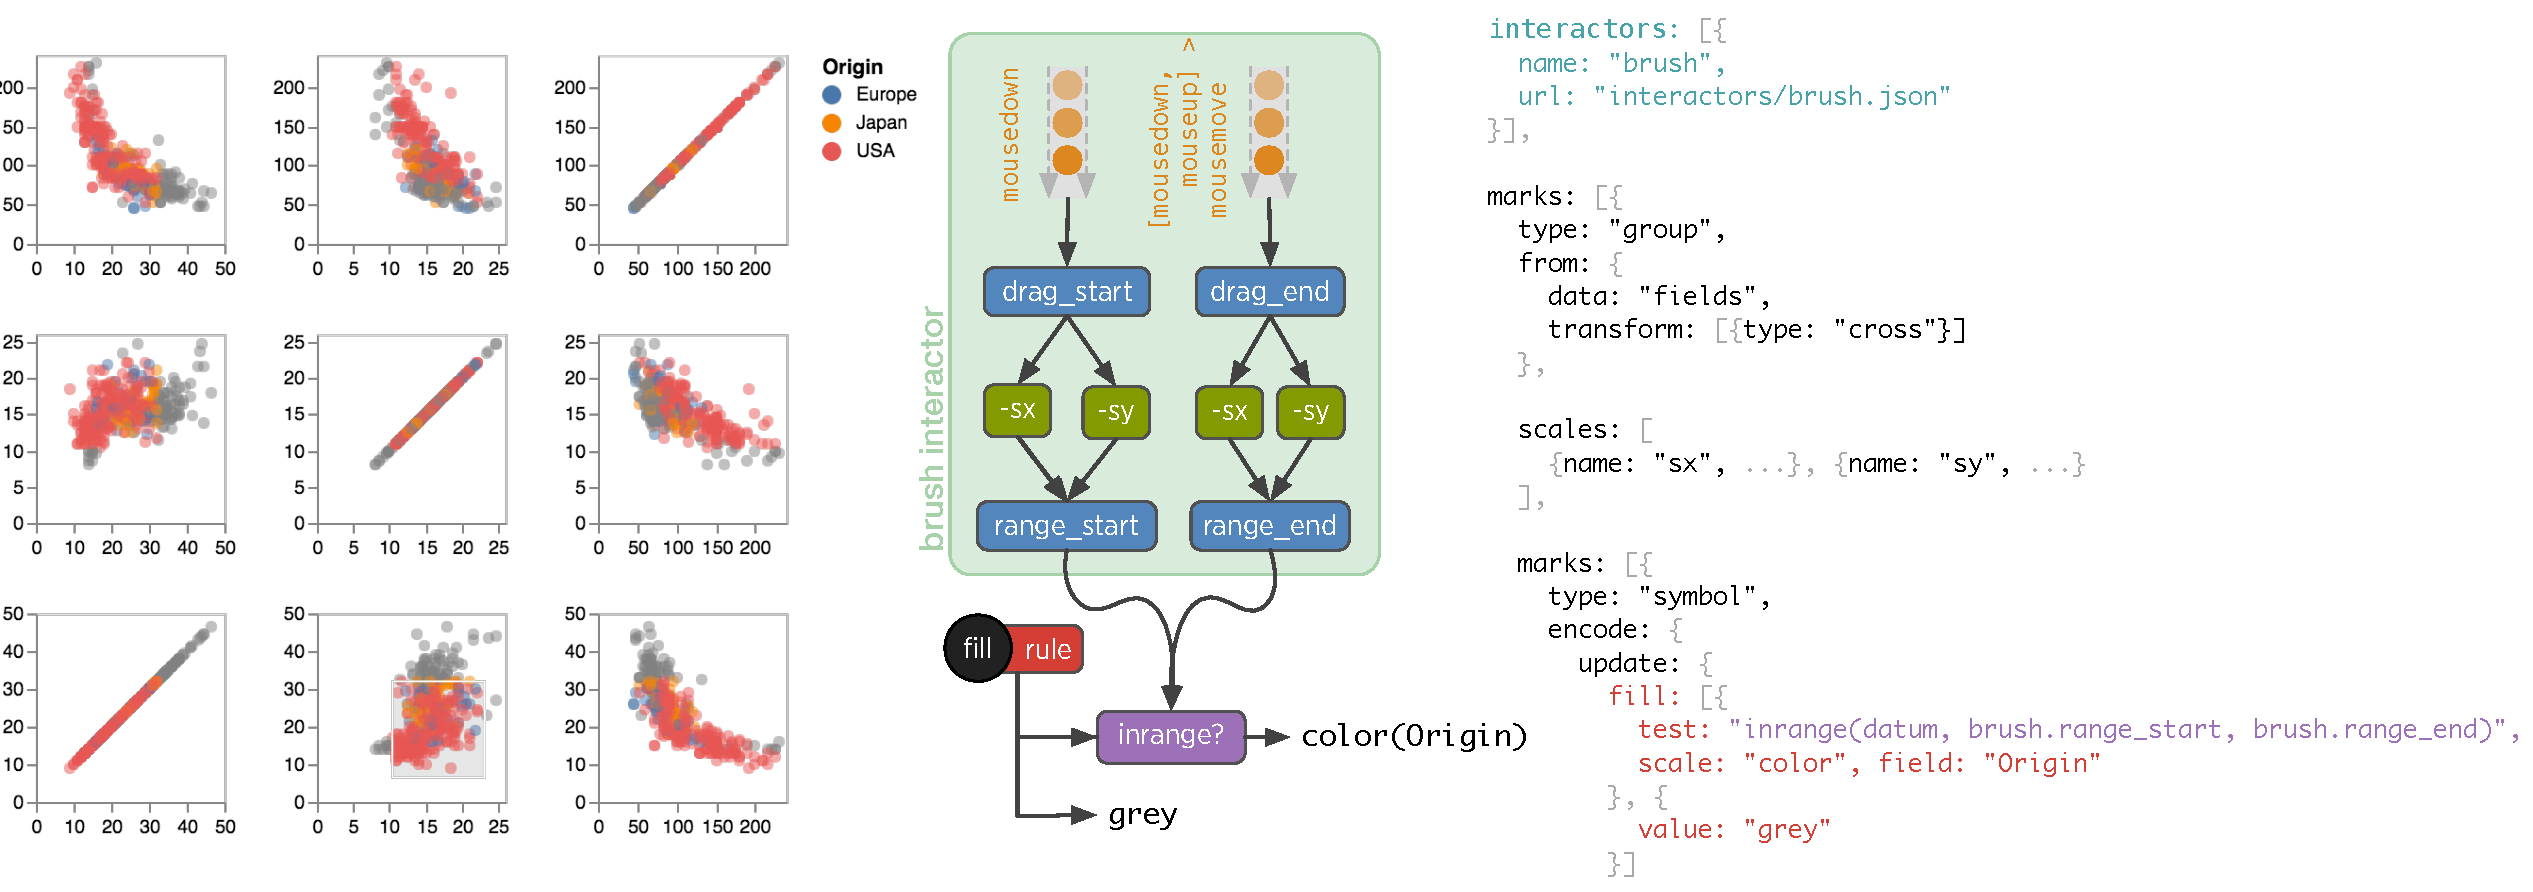
\includegraphics[width=\columnwidth]{splomInteractor}
  \caption{We can extract the brushing interaction from \cref{fig:vg:brush}
  into a standalone interactor, and reapply it to a scatterplot matrix to
  perform brushing \& linking.}
  \label{fig:vg:splomInteractor}
\end{figure}

\subsection{Connect: Brushing \& Linking}

\vspace{-7pt}

\begin{wrapfigure}{l}{0pt}
  \raisebox{0pt}[\dimexpr\height-0.6\baselineskip\relax]{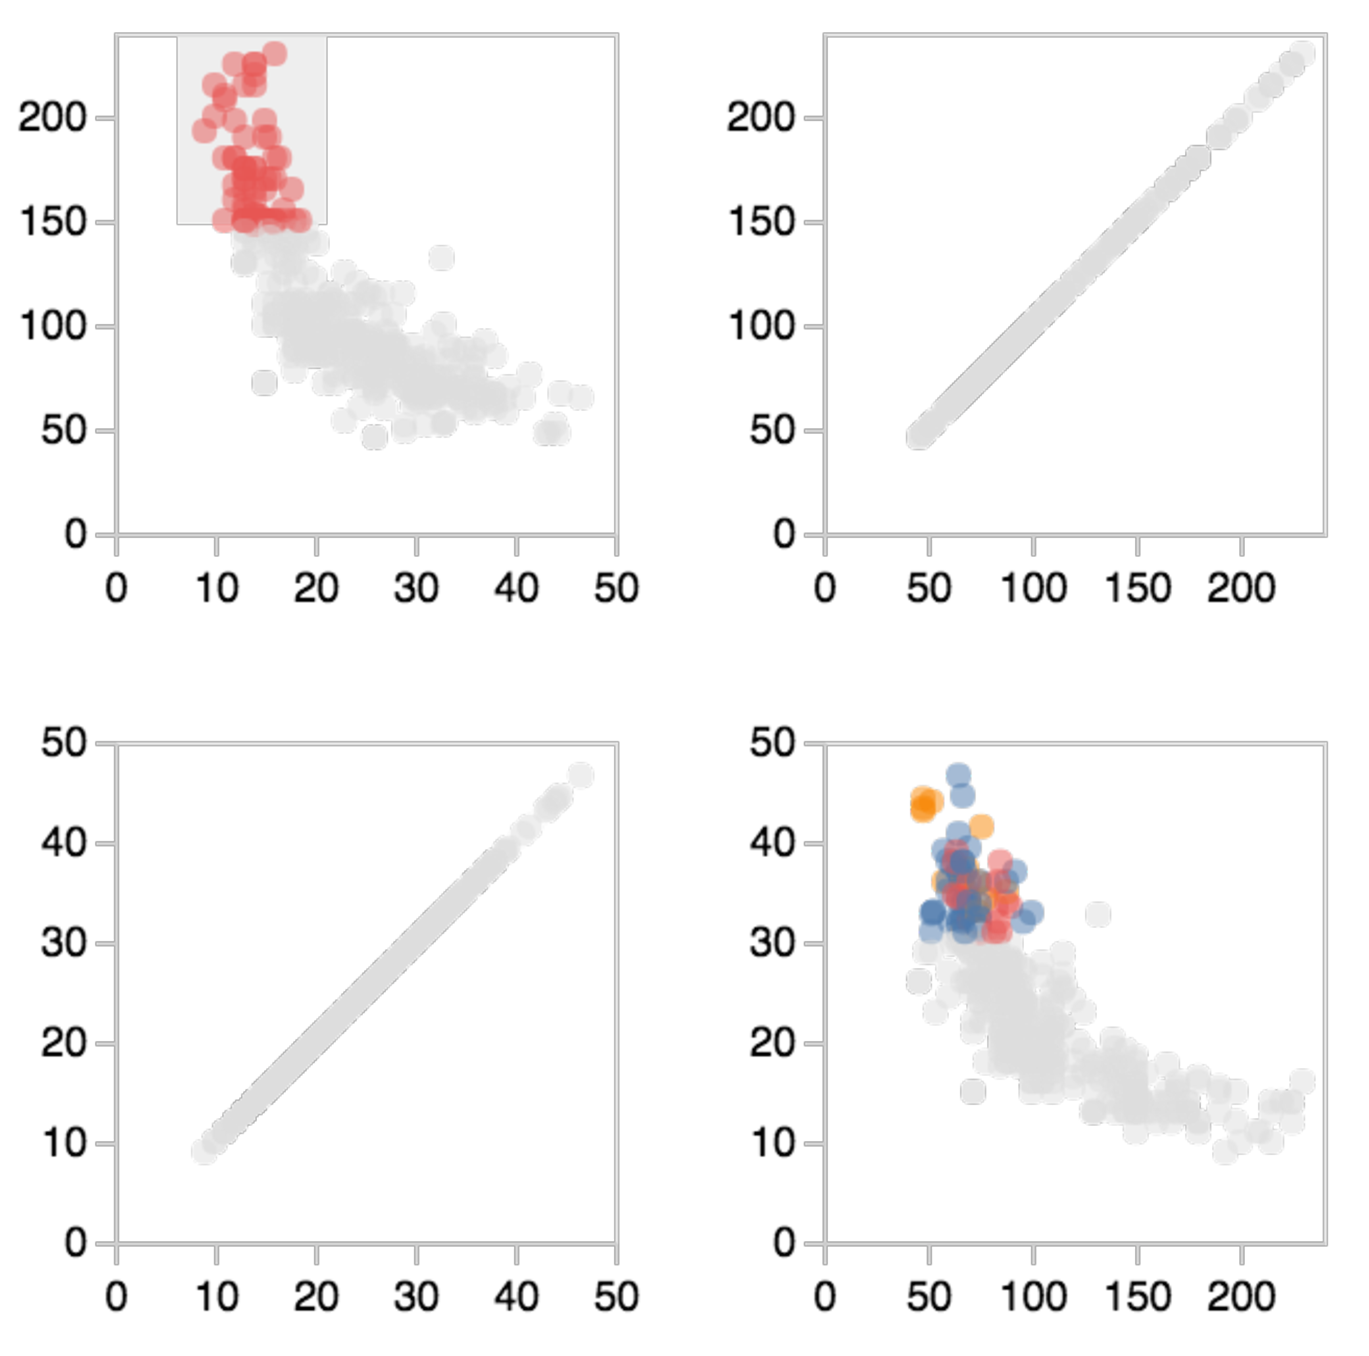
\includegraphics
  [width=0.27\textwidth]{splomPixel}}
\end{wrapfigure}

We can extract the previous interaction into a standalone ``brushing''
interactor, and then apply it to brush \& link a scatterplot matrix as shown in
\cref{fig:vg:splomInteractor}. Each cell of the matrix is an instance of a group
mark with its own coordinate space. The plotting symbol and spatial scale
functions are defined within these groups. Had the interactor's predicates
defined selections over pixel space, the production rule would highlight points
that fall along the same horizontal and vertical pixel regions\,---\,for
example, as shown in the inset figure, brushing over red points would highlight
blue points in the other cells. Instead, the interactor uses scale inversions to
lift the predicate to the data domain, and the production rule correctly links
brushed points across scatterplots.

\vspace{-10pt}

\subsection{Abstract/Elaborate: Overview\,+\,Detail}

\vspace{-7pt}

With our brush interactor, we can also create the overview\,+\,detail
visualization in \cref{fig:vg:scaleInversion}. In this case, brushing is
restricted to the horizontal dimension by overriding the \texttt{height}
property of the interactor's mark, and ignoring the vertical range predicates it
populates. We use the horizontal range predicate with a filter transformation,
to filter points for display in the detail plot. As a user brushes, signals
update the range predicate, which in turn filters points in the data source,
updates scale functions and re-renders the detail view.

\vspace{-10pt}

\subsection{Explore \& Encode: Panning \& Zooming}

\vspace{-7pt}

\begin{figure}[b!]
  \centering
  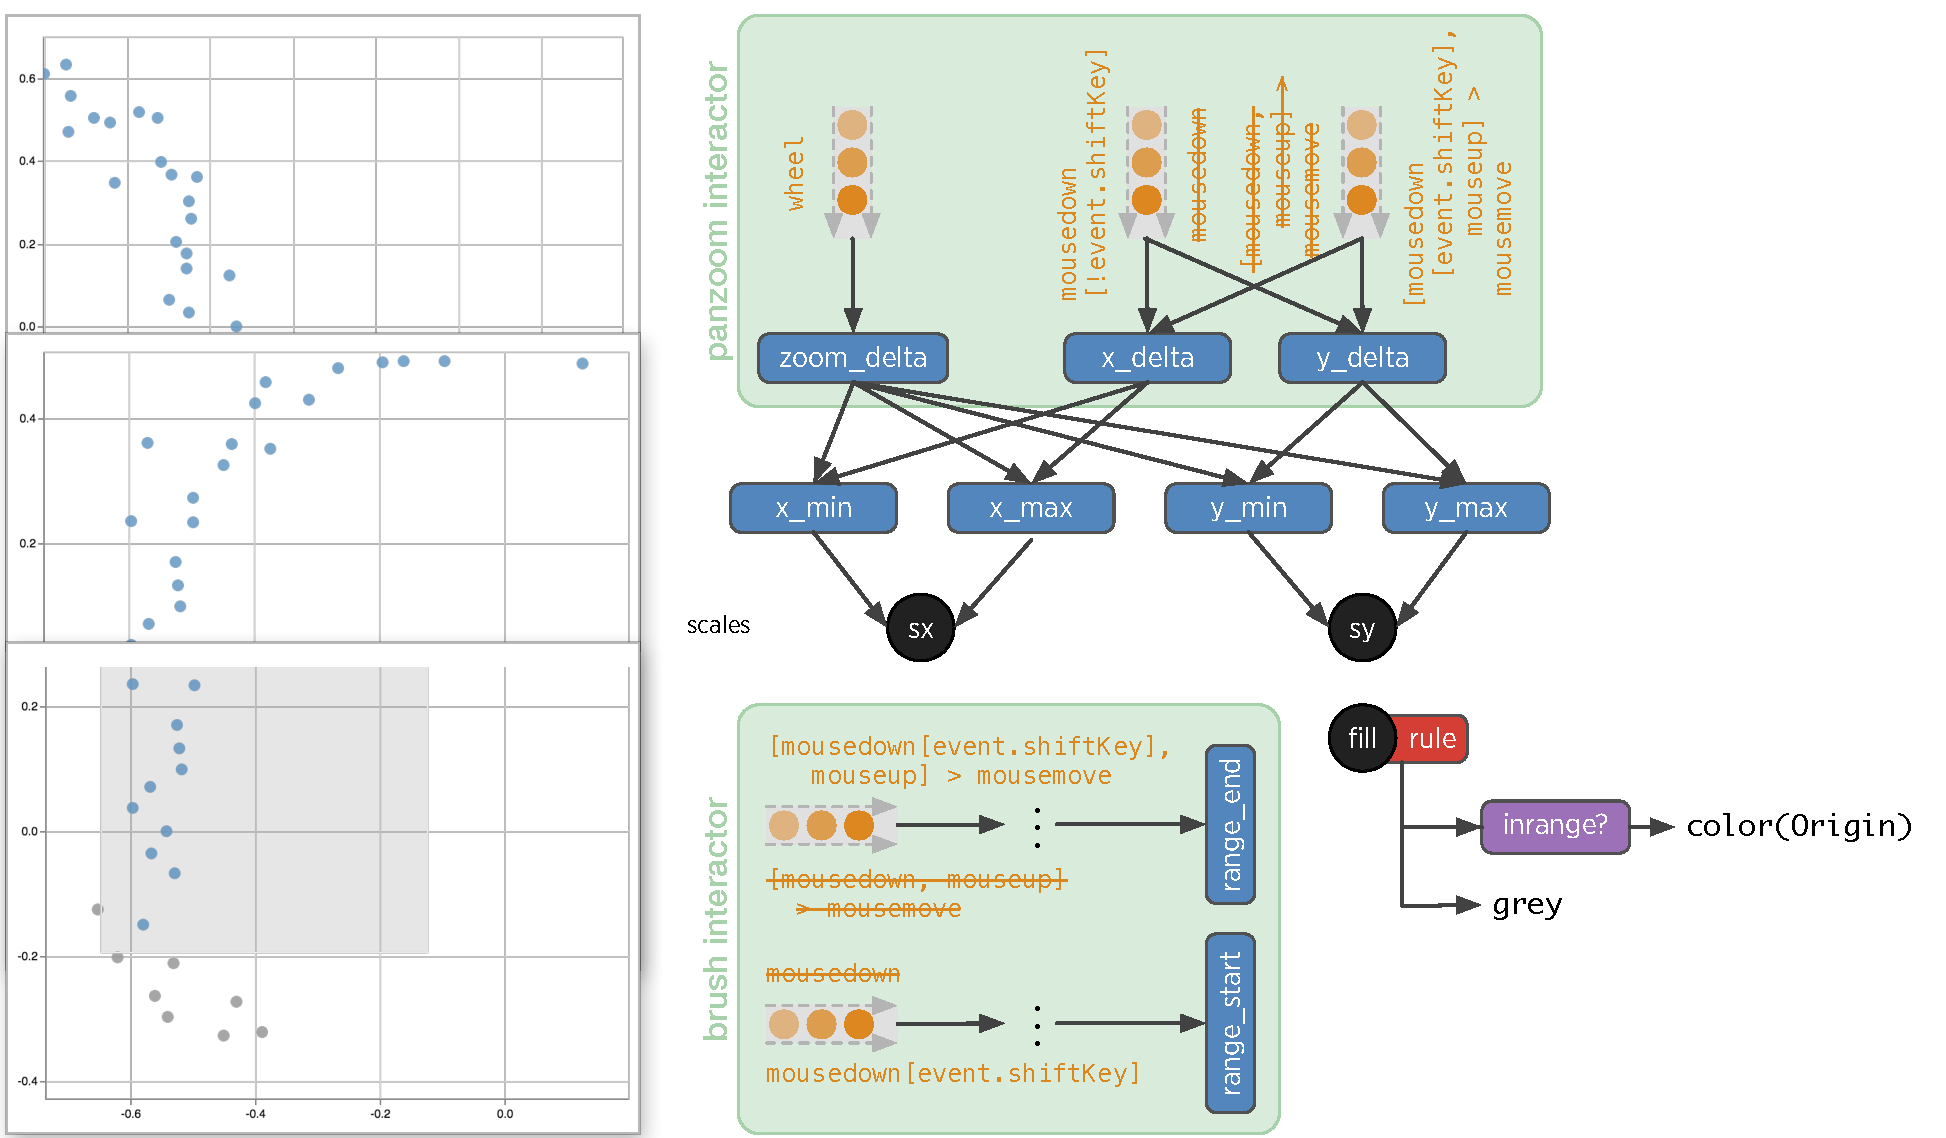
\includegraphics[width=\columnwidth]{panzoom}
  \caption{Panning \& zooming a scatterplot. Brushing is accretively added with
  the brush interactor (\cref{fig:vg:brush,fig:vg:splomInteractor}), and
  conflicts are resolved by rebinding event streams (indicated with
  strikethroughs).}
  \label{fig:vg:panzoom}
\end{figure}

\Cref{fig:vg:panzoom} shows pan and zoom interactions for a scatter plot. By
default, scale functions calculate their domain automatically from a data
source. For this interaction, however, we must parameterize the domain using
reactive signals. For panning, a \texttt{start} signal captures an initial
\texttt{(x,y)} position on \texttt{mousedown}, and subsequent \texttt{pan}
signals calculate a delta on drag (\texttt{[mousedown, mouseup] > mousemove}).
This delta is used to offset the scale domains. Similarly, when \texttt{wheel}
events occur, a \texttt{zoom} signal applies a scale factor to the domains
depending on the zoom direction.

\begin{figure}[b!]
  \centering
  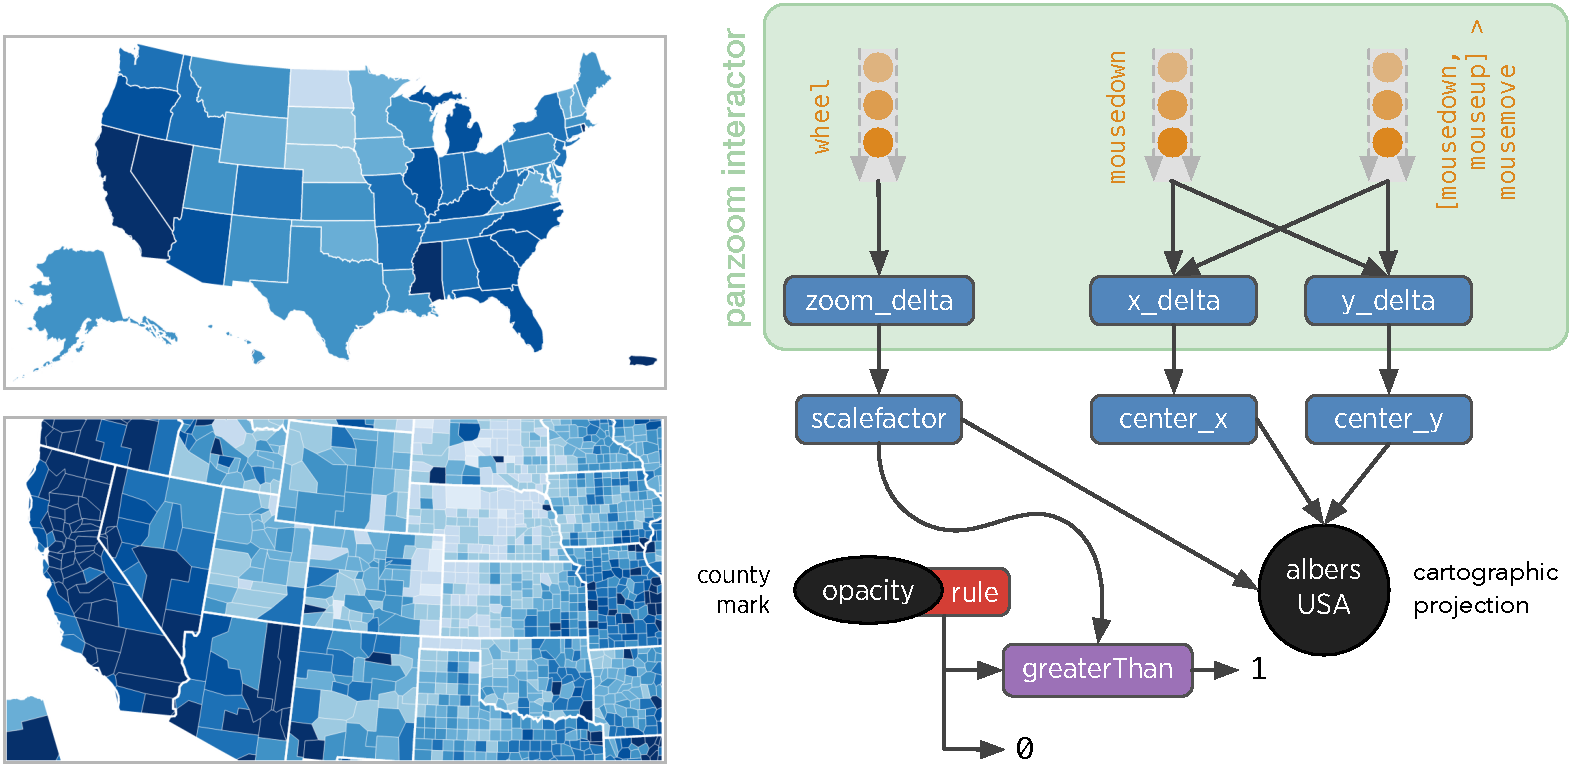
\includegraphics[width=\columnwidth]{semanticZoom}
  \caption{Extracting the pan \& zoom interaction from \cref{fig:vg:panzoom}
  into an interactor, and repurposing it to perform \emph{semantic} zooming on a
  cartographic map. Initially, a choropleth of state-level unemployment in the
  United States is shown. Zooming past a threshold, states break up into
  counties, and show county-level unemployment instead.}
  \label{fig:vg:semanticZoom}
\end{figure}

If we were to also add a brushing interaction to this visualization, a na\"ive
application would yield a conflicting interaction: on drag, both panning and
brushing would occur. One option to resolve this conflict is to begin brushing
only when the shift key is pressed. If we try combining these interactions using
D3~\cite{bostock:d3}, which offers brushing and panning as part of its
interactor typology, specifying this resolution scheme can be onerous.
Additional callbacks must be registered that either instantiate or destroy a
particular interaction depending on the state of the shift key.

With Reactive Vega, the brush and pan signals can be rebound without modifying
the interactor definitions. Instead, we provide alternate source event streams
when instantiating the interactor\,---\,\texttt{mousedown[event.shiftKey]} for
brushing, and\\\texttt{mousedown[!event.shiftKey]} for panning.

Moreover, by extracting panning \& zooming into a standalone interactor, we can
repurpose the behavior to instead trigger semantic zooming~\cite{perlin:pad}, an
\emph{encoding} interaction technique shown in \cref{fig:vg:semanticZoom}. At
the top-level, the visualization shows a choropleth map of state-level
unemployment. After crossing a specified zoom threshold, states subdivide to
show a choropleth map of country-level unemployment. Here, the pan signals drive
the geographic projection's translation and the zoom signals drive the
projection's scale parameter. By default, both maps are drawn with states
overlaying counties. A production rule uses a predicate to test whether the zoom
signal is above a specified threshold; if it is, the state-level map is rendered
transparently, displaying the county-level map underneath it.

\vspace{-10pt}

\subsection{Reconfigure: Index Chart}

\vspace{-7pt}

\begin{figure}[b!]
  \centering
  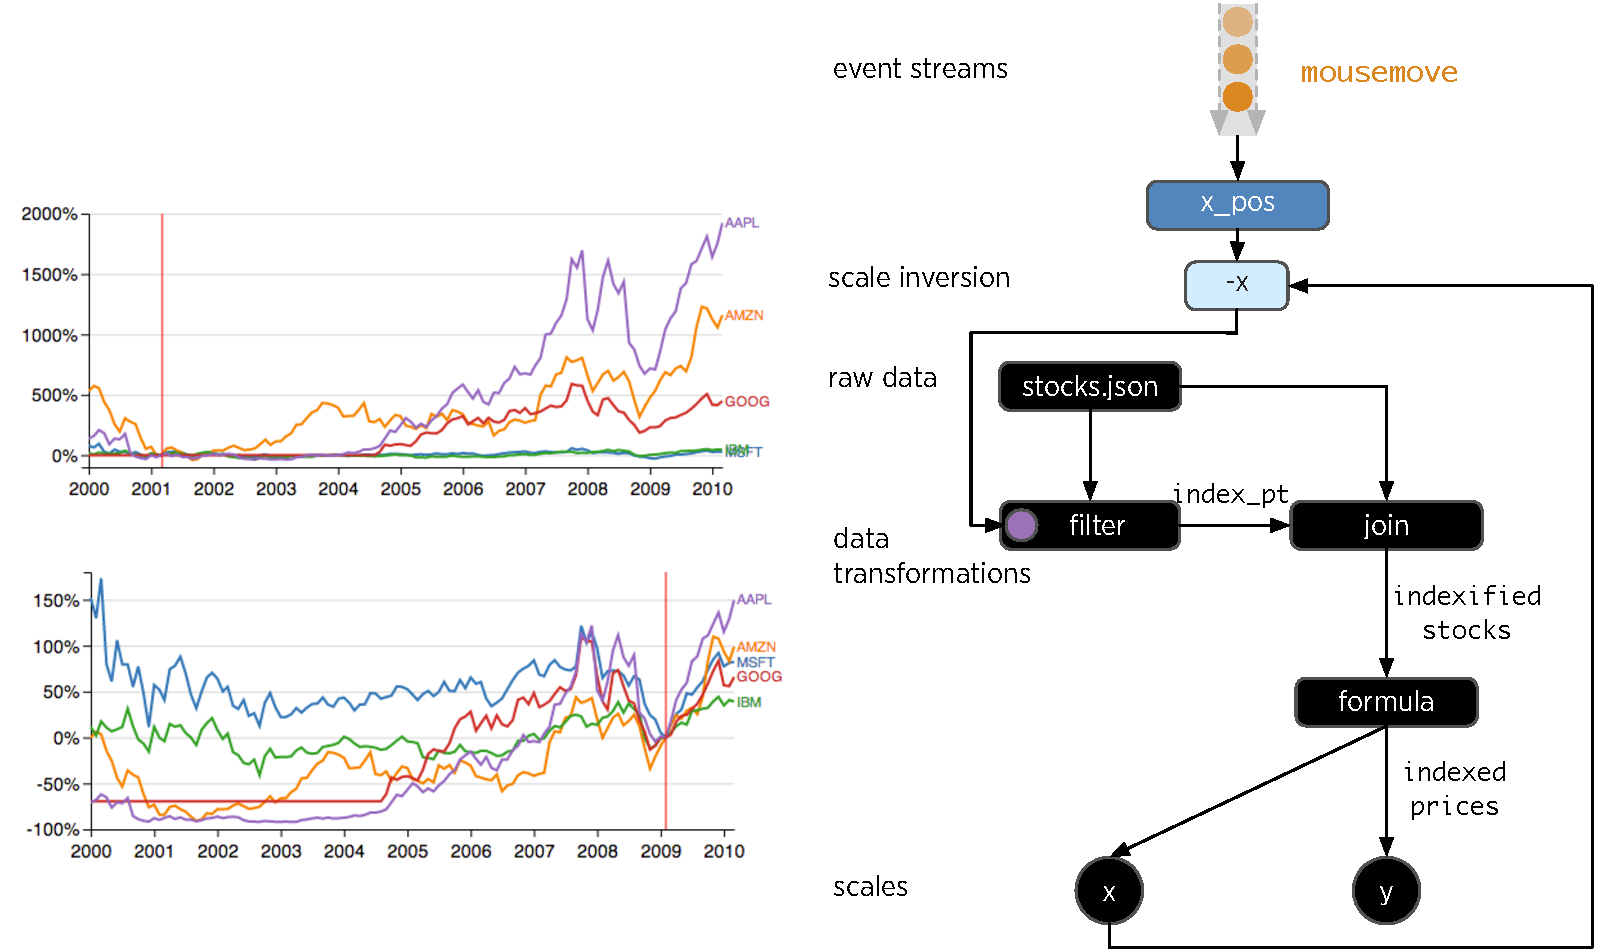
\includegraphics[width=0.89\columnwidth]{indexChart}
  \caption{An index chart shows the percentage changes for time-series data. The
  index point (red vertical line) is determined by the x position of a
  \texttt{mousemove} signal, which filters points using a predicate.}
  \label{fig:vg:indexChart}
\end{figure}

\Cref{fig:vg:indexChart} shows an index chart: a line chart that interactively
normalizes time series to show percentage change based on the current index
point. To calculate the index point, a signal captures the \texttt{x} coordinate
of \texttt{mousemove}events, and drives it through a scale inversion. As it is a
quantitative scale, scale inversion produces a value from a continuous domain
(i.e., any date/time from Jan 1, 2000--Dec 31, 2010). However, our dataset only
contains stock prices for the start of every month. We use a predicate to ``snap
to'' the closest value for each time series, and use this as our index point.
Using Vega's data transformations, we join the index point against the original
data set and normalize the data values. Scale functions are defined in terms of
the normalized data.

\vspace{-10pt}

\subsection{Reconfigure: Reordering Columns of a Matrix}

\vspace{-7pt}

\begin{wrapfigure}{l}{0pt}
  \raisebox{0pt}[\dimexpr\height-0.6\baselineskip\relax]{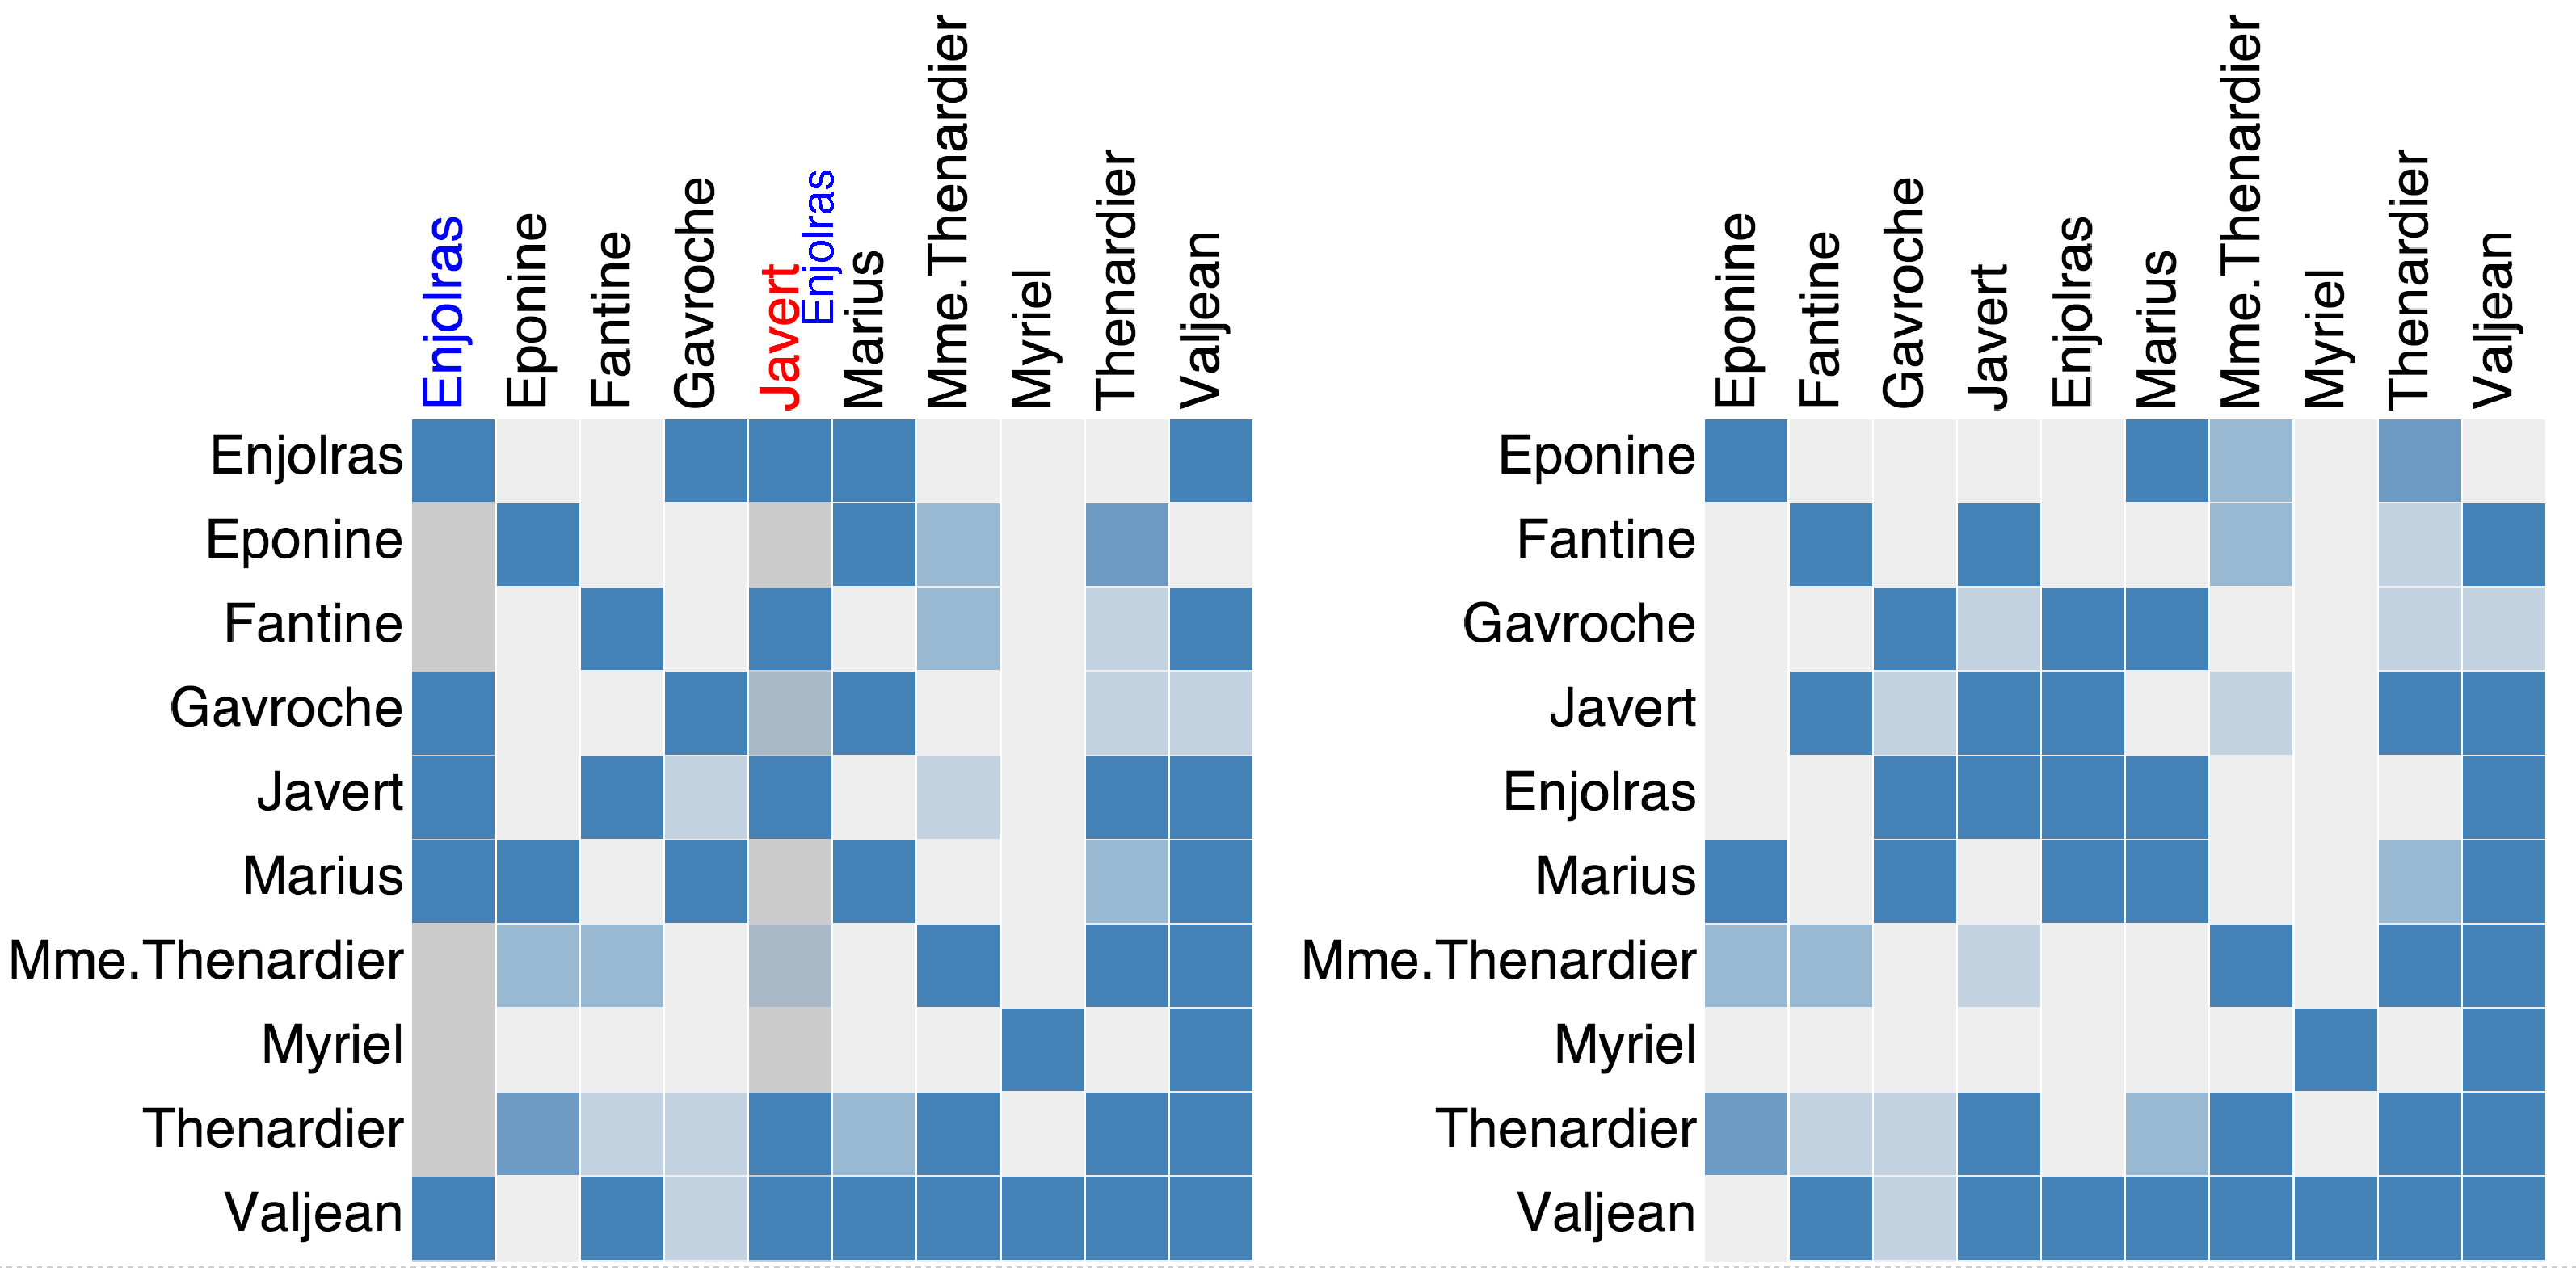
\includegraphics
  [width=0.6\textwidth]{cooccurrence}}
\end{wrapfigure}

\vspace{-7pt}

The figure to the left shows a co-occurrence matrix of Les Mis\'{e}rables
characters. To reorder the columns of the matrix, we first construct a data
source that computes the sort order of characters and initialize it to an
alphabetical ordering. A signal on \texttt{@col\_label:mousedown} captures the
source column to be reordered, while a signal on \texttt{[@col\_label:mousedown,
mouseup] > mousemove} updates the target column location. On \texttt{mouseup},
the data source is updated to swap the two sorting indices.

\vspace{-10pt}

\subsection{Filter: Control Widgets}

\vspace{-7pt}

\begin{figure}[t!]
  \centering
  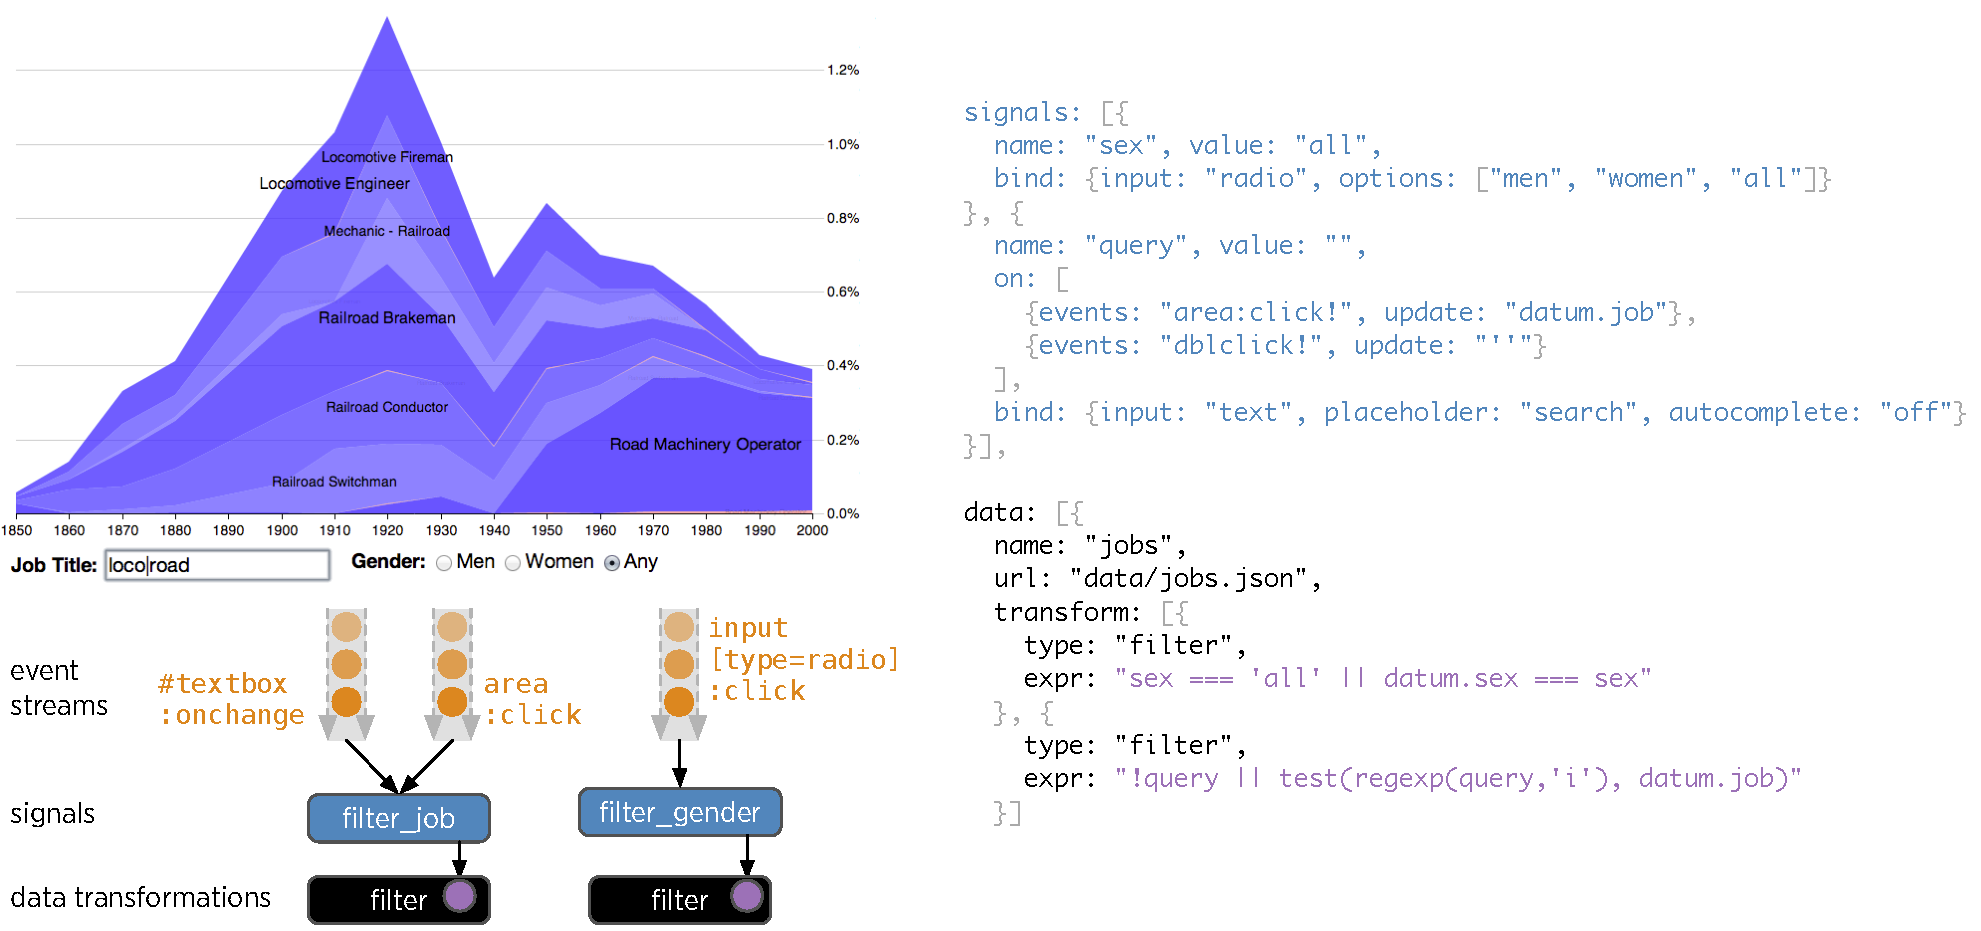
\includegraphics[width=0.9\columnwidth]{jobVoyager}
  \caption{The job voyager can be filtered using signals bound to control
  widgets. The textbox pattern matches against job titles while radio buttons
  filter by gender.}
  \label{fig:vg:jobVoyager}
\end{figure}

\Cref{fig:vg:jobVoyager} shows the Job Voyager~\cite{heer:voyagers}
visualization with control widgets to filter the visualized data. A textbox
allows users to enter search terms to filter job titles, while the radio buttons
allow users to filter by gender. We bind signals to the value of these control
widgets, and then construct predicates attached to filter data transformations.
For the textbox signal, a regular expression tests terms against job titles,
while an equality test filters by gender based on the radio button signal. This
example illustrates how external widgets can easily be bound to our reactive
model.

\vspace{-20pt}

\subsection{DimpVis: Touch Navigation with Time-Series Data}

\vspace{-7pt}

DimpVis~\cite{kondo:dimpvis} is a recently introduced interaction technique that
allows direct manipulation navigation of time-series data. Starting with a
scatterplot depicting data at a particular time slice, users can touch plotted
points to reveal a ``hint path'': a line graph that displays the trajectory of
the selected element over time. Dragging the selected point along this path
triggers temporal navigation, with the rest of the points updating to reflect
the new time. In evaluation studies, users reported feeling more engaged when
exploring their data using DimpVis~\cite{kondo:dimpvis}.

As shown in \cref{fig:vg:dimpvis}, we can recreate this technique with Reactive
Vega's declarative interaction primitives and the GapMinder
country-fertility-life-expectancy dataset used by the original. Input data is
passed through a \texttt{Window} transform, such that every tuple contains
references to the tuples that come before and after it in time, and filtered to
remove triplets that span multiple countries. Signals constructed over mouse and
touch events capture the selected point, and downstream signals calculate
distances between the user's current position and the previous and next points.
A scalar projection over these distances gives us scoring functions that
determine whether the user is moving forwards or backwards in time. Scores feed
a signal that is used in a derived data source to calculate new interpolated
properties for the remaining points in the dataset. These interpolated
properties determine the position of plotted points, producing smooth
transitions as the user drags back-and-forth. To draw the hint map, a derived
data source filters data tuples for the selected country across all years.

\begin{figure}[h!]
  \centering
  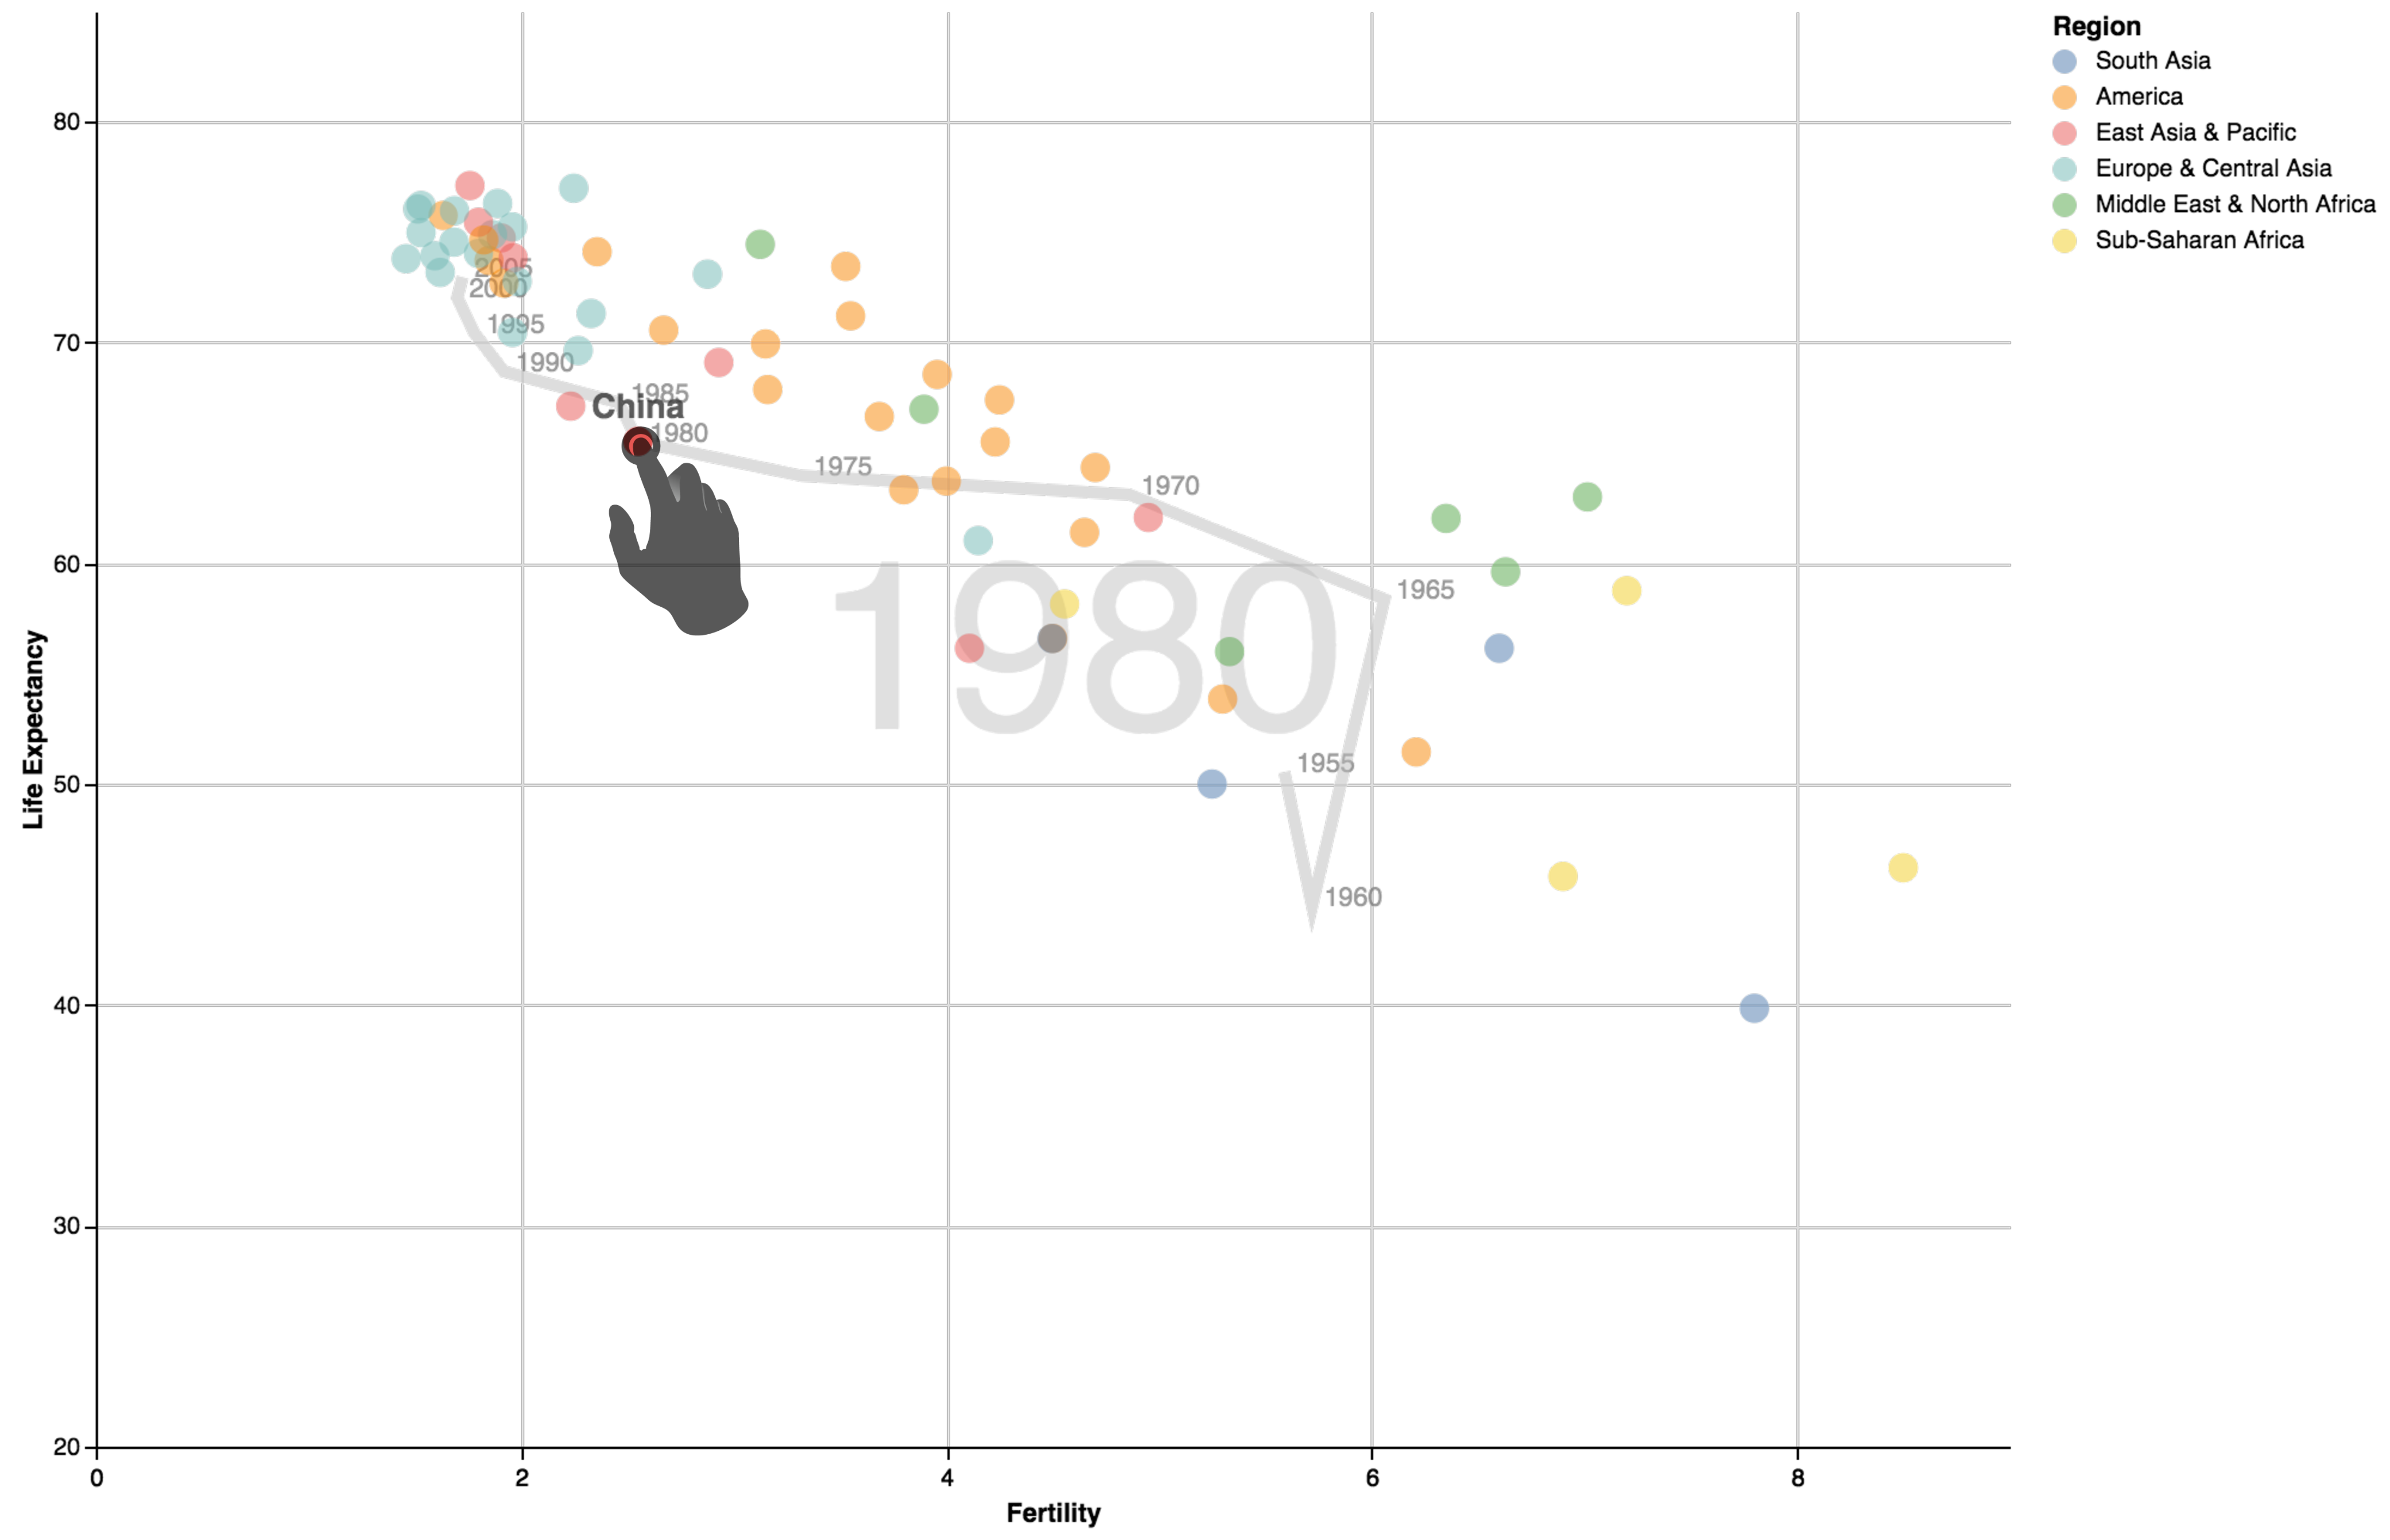
\includegraphics[width=\columnwidth]{dimpvis}
  \caption{DimpVis~\cite{kondo:dimpvis}, touch-based navigation of time-series
  data recreated with Reactive Vega.}
  \label{fig:vg:dimpvis}
\end{figure}

\vspace{-10pt}

\subsection{Reusable Touch Interaction Abstractions}

\vspace{-7pt}

With the proliferation of touch-enabled devices, particularly smartphones and
tablets, supporting touch-based interaction has become an increasingly important
part of interactive visualization design. However, HTML5 only provides a
low-level API for touch events, with three event types broadly
supported\,---\,\texttt{touchstart}, \texttt{touchmove}, and \texttt{touchend}.
On multitouch devices these events contain an array of touch points. The
application developer is responsible for the bookkeeping involved with tracking
multiple points across interactions, a cumbersome and difficult process.

Declarative interaction design enables us to abstract low-level details away,
building reusable interactors that expose higher-level, semantic events as
signals instead. For example, an interactor could define signals that perform
the necessary logic for common multitouch gestures. Once such an interactor is
included in a host visualization, the visualization designer can then safely
ignore lower-level events, and instead build interactions driven by the
interactor's signals\,---\,using \texttt{twotouchmove} and \texttt{pinchDelta}
signals to drive panning and zooming behaviors, for instance.
% !TEX root = ../thesis.tex
\section{Discussion: Cognitive Dimensions of Notation}
\label{sec:vg:discussion}

The previous section demonstrated the expressivity of Reactive Vega's model of
declarative interaction design. Here, we evaluate it from the perspective of a
visualization designer using the Cognitive Dimensions of
Notation~\cite{blackwell:cogdim}, a set of heuristics for evaluating the
efficacy of notational systems such as programming languages and interfaces. Of
the 14 dimensions, we evaluate Reactive Vega against a relevant subset and
compare it against current common practice: declarative specification of visual
encodings using D3~\cite{bostock:d3} and imperative event handling callbacks for
interaction.

\textbf{Abstractions} (types and availability of abstraction mechanisms) and
\textbf{Viscosity} (resistance to change). Streams and signals abstract the
low-level events that trigger interactions and decouple them from downstream
logic. This approach can facilitate rapid iteration: the result of an
interaction can be designed (for example, highlighting points), and then a
variety of different event triggers can be prototyped by simply rebinding the
appropriate signals. As our examples demonstrate, rebinding signals reduces the
burden for resolving conflicting interactions or retargeting to different
platforms. By comparison, iterating with event callbacks can be more difficult.
A particular sequence of events may require a specific ordering of callbacks,
and coordinating the visualization state across these functions falls to the
designer.

\textbf{Premature Commitment} (constraints on the order of doing things).
Abstracting streams into signals does impose a premature commitment. Users must
define them before they are able to use any lower-level events to trigger state
changes. This requirement could be relaxed: users could use event streams
inline, for example within a predicate or production rule. However, we believe
such inline references are a poor design pattern as they make an interaction
technique dependent on a specific set of events\,---\,a common problem with
existing interactor typologies. Moreover, reuse would be hampered as it would
become more difficult to resolve conflicting interactions (e.g., brushing and
panning) or retarget techniques across input modalities.

\textbf{Hidden Dependencies} (important links between entities are not visible).
Signals do introduce hidden dependencies as they obscure which input events
trigger particular changes to the state of the visualization. However, we
believe that the gains in viscosity outweigh the complexities of these hidden
dependencies, particularly as the latter can be ameliorated by naming signals
appropriately. Furthermore, as our code examples illustrate, all the factors
that directly affect a particular state are captured within a single Reactive
Vega specification. For example, a signal definition specifies all events or
signals that may affect its value; similarly, a visual property may use a rule
which enumerates all the values it may take. With D3, the visual encoding
specification may not completely define all states. Instead, the user must trace
a flow through event callbacks, a process further exacerbated by an
unpredictable execution order. The user is forced to coordinate interleaved
callbacks, introducing \textbf{hard mental operations} and
\textbf{error-proneness}.

\textbf{Consistency} (similar semantics are expressed in similar syntactic
forms). Our interaction model is best suited for systems that declaratively
specify visual encodings, and would feel foreign in imperative systems. However,
given the widespread adoption of D3, and Vega's increasing integration in
systems~\cite{lyra, voyager, wikipedia:graph} we believe this is not a
significant liability. By contrast, registering event callbacks on D3
visualizations breaks consistency: visual design is declarative while
interaction design is imperative. It requires users to think in terms of
different notational systems, and exposes underlying implementation and
execution concerns.

\textbf{Visibility} (ability to view components easily). One of the primary
advantages of using D3, and registering event callbacks, is being able to debug
code directly within a web browser~\cite{bostock:d3}: the generated
visualization can be inspected, while the JavaScript console can be used to
interactively debug event callbacks. Reusing such existing scaffolding is more
difficult with Reactive Vega as its runtime, which parses and renders a
specification, introduces its own stack of abstractions. However, we believe
this gap offers a promising avenue for future work in new development
environments that can leverage Vega's reactive semantics. For instance, initial
work by Hoffswell et al.~\cite{hoffswell:debugging} has devised a
``time-travelling'' debugger for Reactive Vega specifications. In particular,
the authors note that signals are a critical abstraction barrier, providing a
meaningful entry-point into an interaction specification. To construct a similar
debugger for imperative event handling callbacks would require complex static
analysis to identify and surface relevant program state.

In summary, Reactive Vega introduces hidden dependencies between state changes
and their triggering input events and, without additional tooling, decreases
visibility into runtime execution. However, we believe these drawbacks are
outweighed by the increase in specification consistency between visual encodings
and interaction, and a decrease in viscosity, allowing users to iterate more
quickly over interaction design.

% !TEX root = ./thesis.tex
\graphicspath{{./vega-arch/figures/}}
\chapter{A Streaming Dataflow Architecture}
\label{sec:vg:arch}

\begin{figure}[h!]
  \vspace{-40pt}
  \centering
  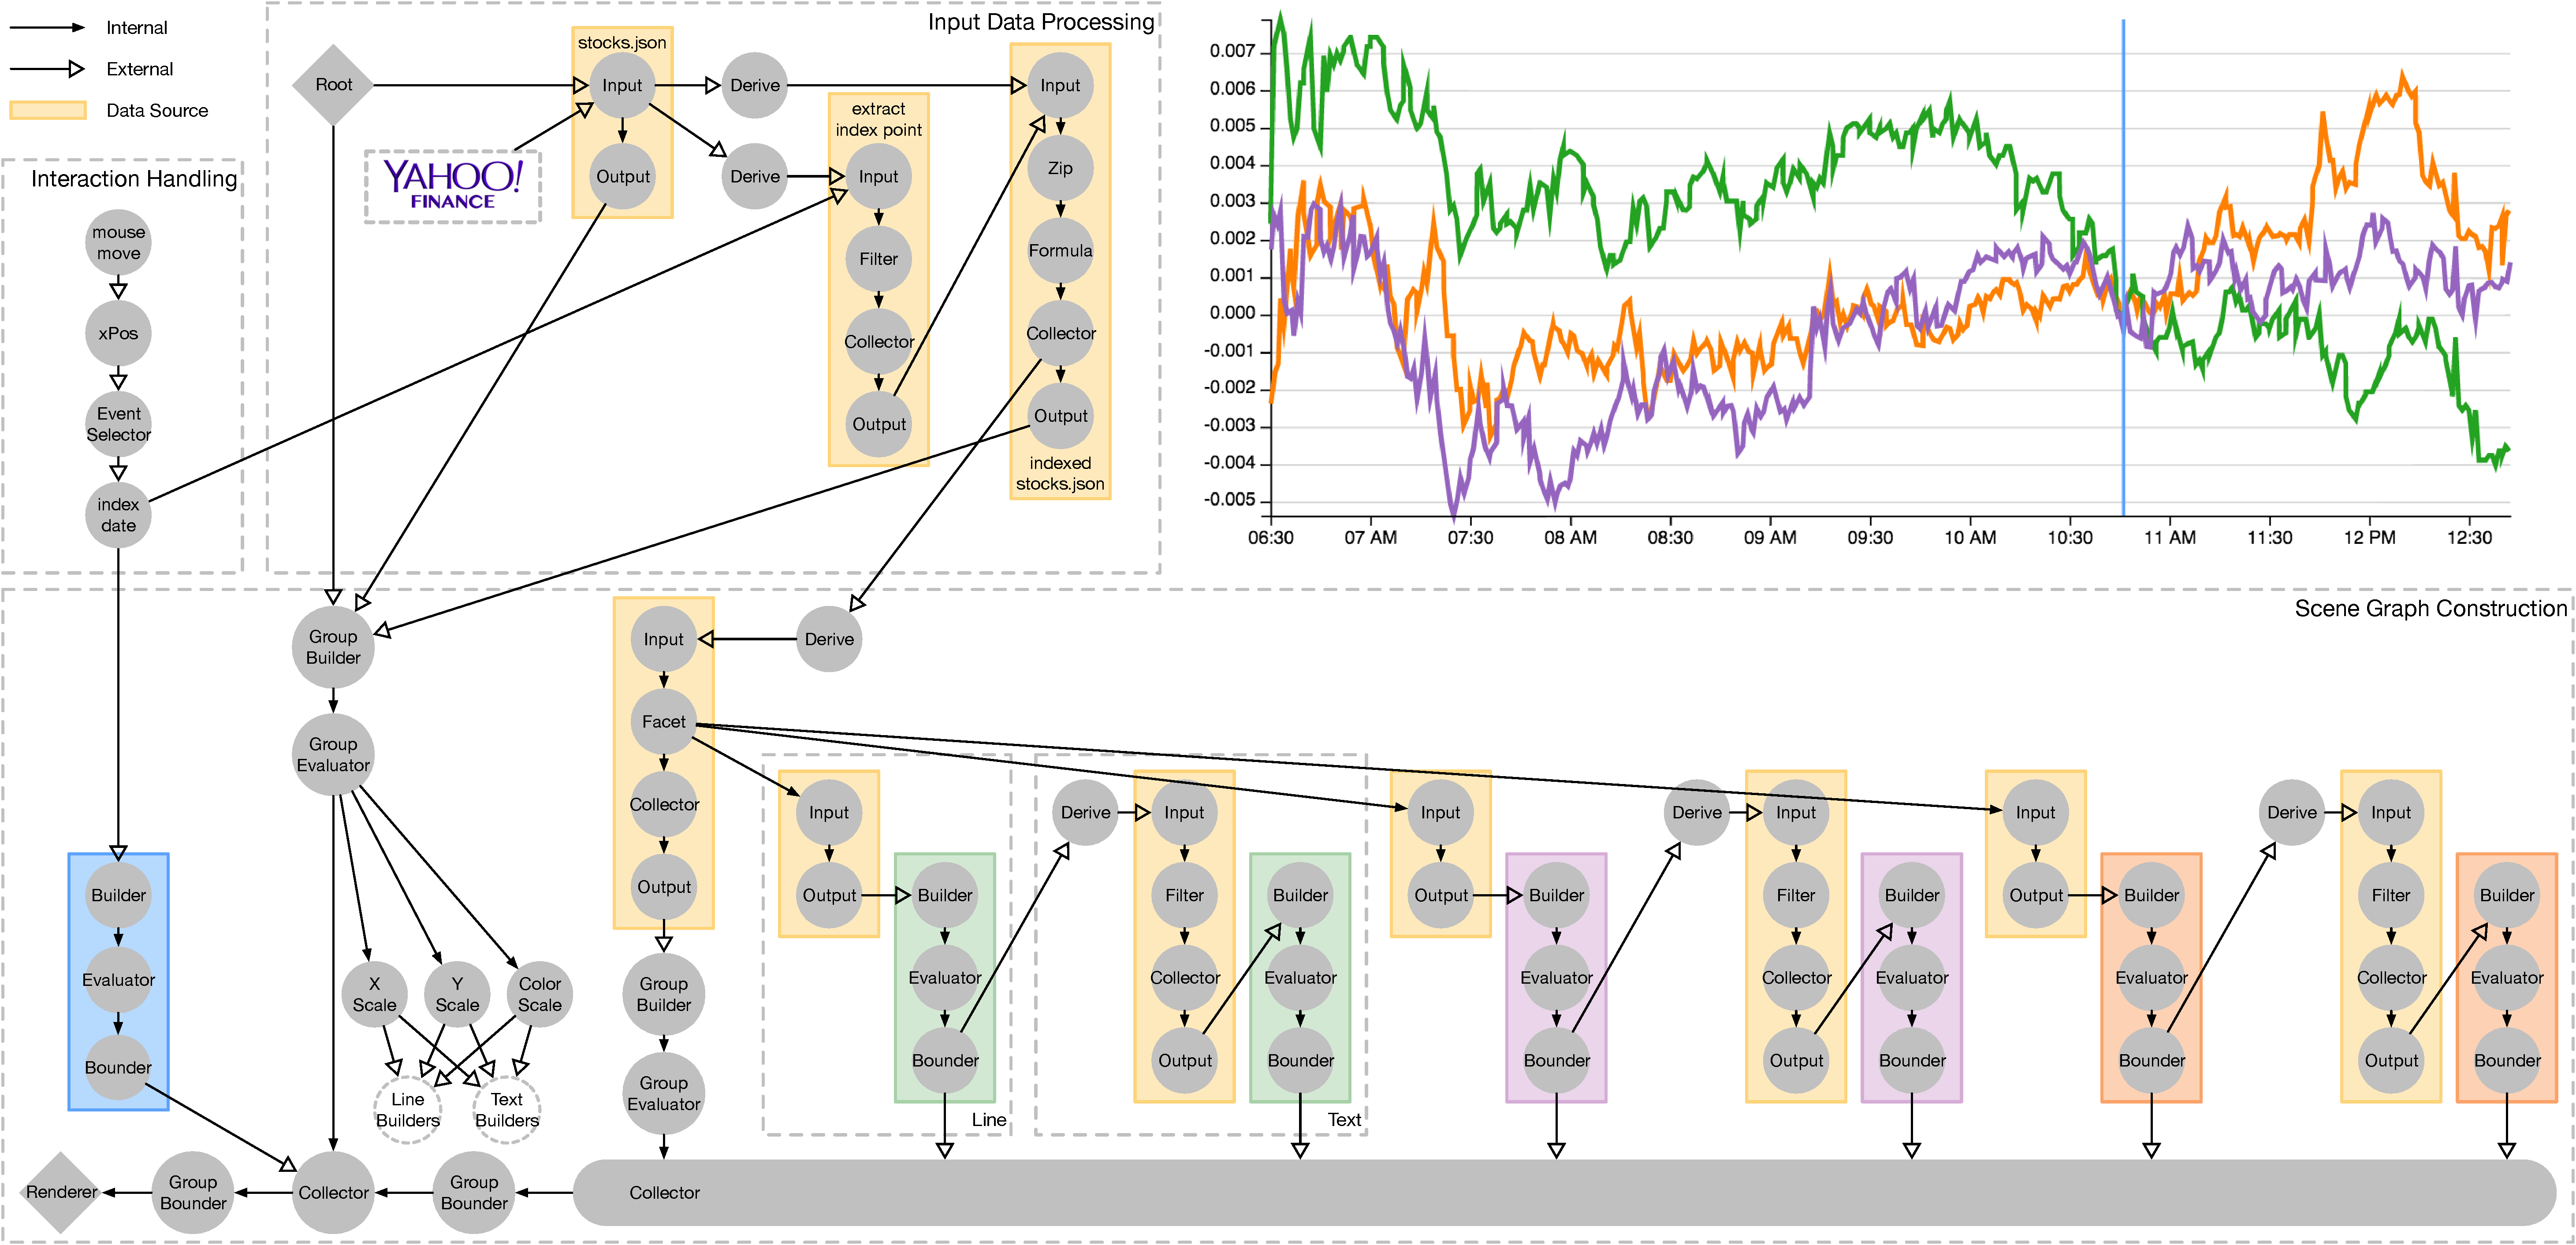
\includegraphics[width=\columnwidth]{teaser}
  \caption{The Reactive Vega dataflow graph created for a interactive index
  chart of streaming financial data. As streaming data arrives from the Yahoo!
  Finance API, or as a user moves their mouse pointer across the chart, an
  update cycle propagates through the graph and triggers an efficient update and
  re-render of the visualization.}
  \label{fig:vg:teaser}
\end{figure}

While the previous chapter describes the design of Reactive Vega's declarative
interaction design model, we now turn to the system architecture needed to
support it. Our architecture design is motivated by four primary goals:

\begin{enumerate}
  \item \textbf{A Unified Data Model}. Existing reactive visualization
toolkits (e.g., Model.js~\cite{kelleher:modeljs}) feature fragmented
architectures where only interaction events are modeled as time-varying. Other
input datasets remain static and batch-processed. This artificial disconnect
restricts expressivity and can result in wasteful computation. For example,
interaction events that manipulate only a subset of input tuples may trigger
recomputation over the entire dataset. In contrast, Reactive Vega features a
unified data model in which input data, scene graph elements, and interaction
events are all treated as first-class streaming data sources.

  \item \textbf{Streaming Relational Data}. Modeling input relational data with
Event-Driven Functional Reactive Programming (E-FRP)~\cite{wan:efrp} semantics
alone does not supply sufficient granularity for targeted recomputation. As
E-FRP semantics consider only time-varying scalar values, operators would
observe an entire relation as having changed and so would need to reprocess all
tuples. Instead, Reactive Vega integrates techniques from streaming
databases~\cite{abadi:borealis, abadi:aurora, arasu:stream, avnur:eddies,
chandrasekaran:telegraphcq} alongside E-FRP, including tracking state at the
tuple-level and only propagating modified tuples through the dataflow graph.

  \item \textbf{Streaming Nested Data}. Interactive visualizations, particularly
those involving small multiples, often require hierarchical structures.
Processing such data poses an additional challenge not faced by prior reactive
or streaming database systems. To support streaming nested data, Reactive Vega's
dataflow graph rewrites itself in a data-driven fashion at runtime: new branches
are extended, or existing branches pruned, in response to observed hierarchies.
Each dataflow branch models its corresponding part of the hierarchy as a
standard relation, enabling operators to remain agnostic to higher-level
structure.

  \item \textbf{Interactive Performance}. Reactive Vega performs both compile-
and run-time optimizations to increase throughput and reduce memory footprint,
including tracking metadata to prune unnecessary computation, and optimizing
scheduling by inlining linear chains of operators. We conduct benchmark
studies of streaming and interactive visualizations and find that Reactive
Vega meets or exceeds the performance of both D3 and the original, unreactive
Vega system.
\end{enumerate}

Reactive Vega is implemented in the JavaScript programming language, and is
intended to run either in a web browser or server-side using Node.js. By
default, Reactive Vega renders to an HTML5 Canvas element; however, it also
supports Scalable Vector Graphics (SVG) and server-side image rendering.

% !TEX root = ../thesis.tex
\section{The Dataflow Graph Design}
\label{sec:vg:dataflow}

Operators in Reactive Vega's dataflow graph are instantiated and connected by
its \emph{parser}, which traverses a declarative specification containing
definitions for input datasets, visual encoding rules, and interaction
primitives as described in~\cref{sec:vg:lang}. When data tuples are observed, or
when interaction events occur, they are propagated (or ``\emph{pulsed}'')
through the graph with each operator being evaluated in turn. Propagation ends
at the graph's sole sink: the renderer.

\subsection{Data, Interaction, and Scene Graph Operators}

Reactive Vega's dataflow operators fall into one of three categories: input data
processing, interaction handling, or scene graph construction.

\subsubsection{Processing Input Data}

Reactive Vega parses each dataset definition and constructs a corresponding
branch in the dataflow graph. These branches comprise input and output nodes
connected by a pipeline of data transformation operators. Input nodes receive
raw tuples as a linear stream (tree and graph structures are supported via
parent-child or neighbor pointers, respectively). Upon data source updates,
tuples are flagged as either \emph{added}, \emph{modified}, or \emph{removed},
and each tuple is given a unique identifier. Data transformation operators use
this metadata to perform targeted computation and, in the process, may derive
new tuples from existing ones. Derived tuples retain access to their ``parent''
via prototypal inheritance\,---\,operators need not propagate unrelated upstream
changes.

Some operators require additional inspection of tuple state. Consider an
aggregate operator that calculates running statistics over a dataset (e.g.,
mean and variance). When the operator observes added or removed tuples, the
statistics can be updated based on the current tuple values. With modified
tuples, the previous value must be subtracted from the calculation and the new
value added. Correspondingly, tuples include a \texttt{previous} property.
Writes to a tuple attribute are done through a setter function that copies
current values to the \texttt{previous} object.

\subsubsection{Handling Interaction}

Reactive Vega instantiates an event listener node in the dataflow graph for each
low-level event type required by the visualization (e.g., \texttt{mousedown} or
\texttt{touchstart}). These nodes are directly connected to dependent signals as
specified by event selectors~\cite{satyanarayan:declarative}. In the case of
ordered selectors (e.g., a ``drag'' event specified by \texttt{[mousedown,
mouseup] > mousemove}), each constituent event is connected to an automatically
created anonymous signal; an additional anonymous signal connects them to serve
as a gatekeeper, and only propagates the final signal value when appropriate.
Individual signals can be dependent on multiple event nodes and/or other
signals, and value propagation follows E-FRP's two-phase update~\cite{wan:efrp}
as described in~\secref{sec:propagation}.

\subsubsection{Constructing the Scene Graph}

\begin{figure}[h!]
  \centering
  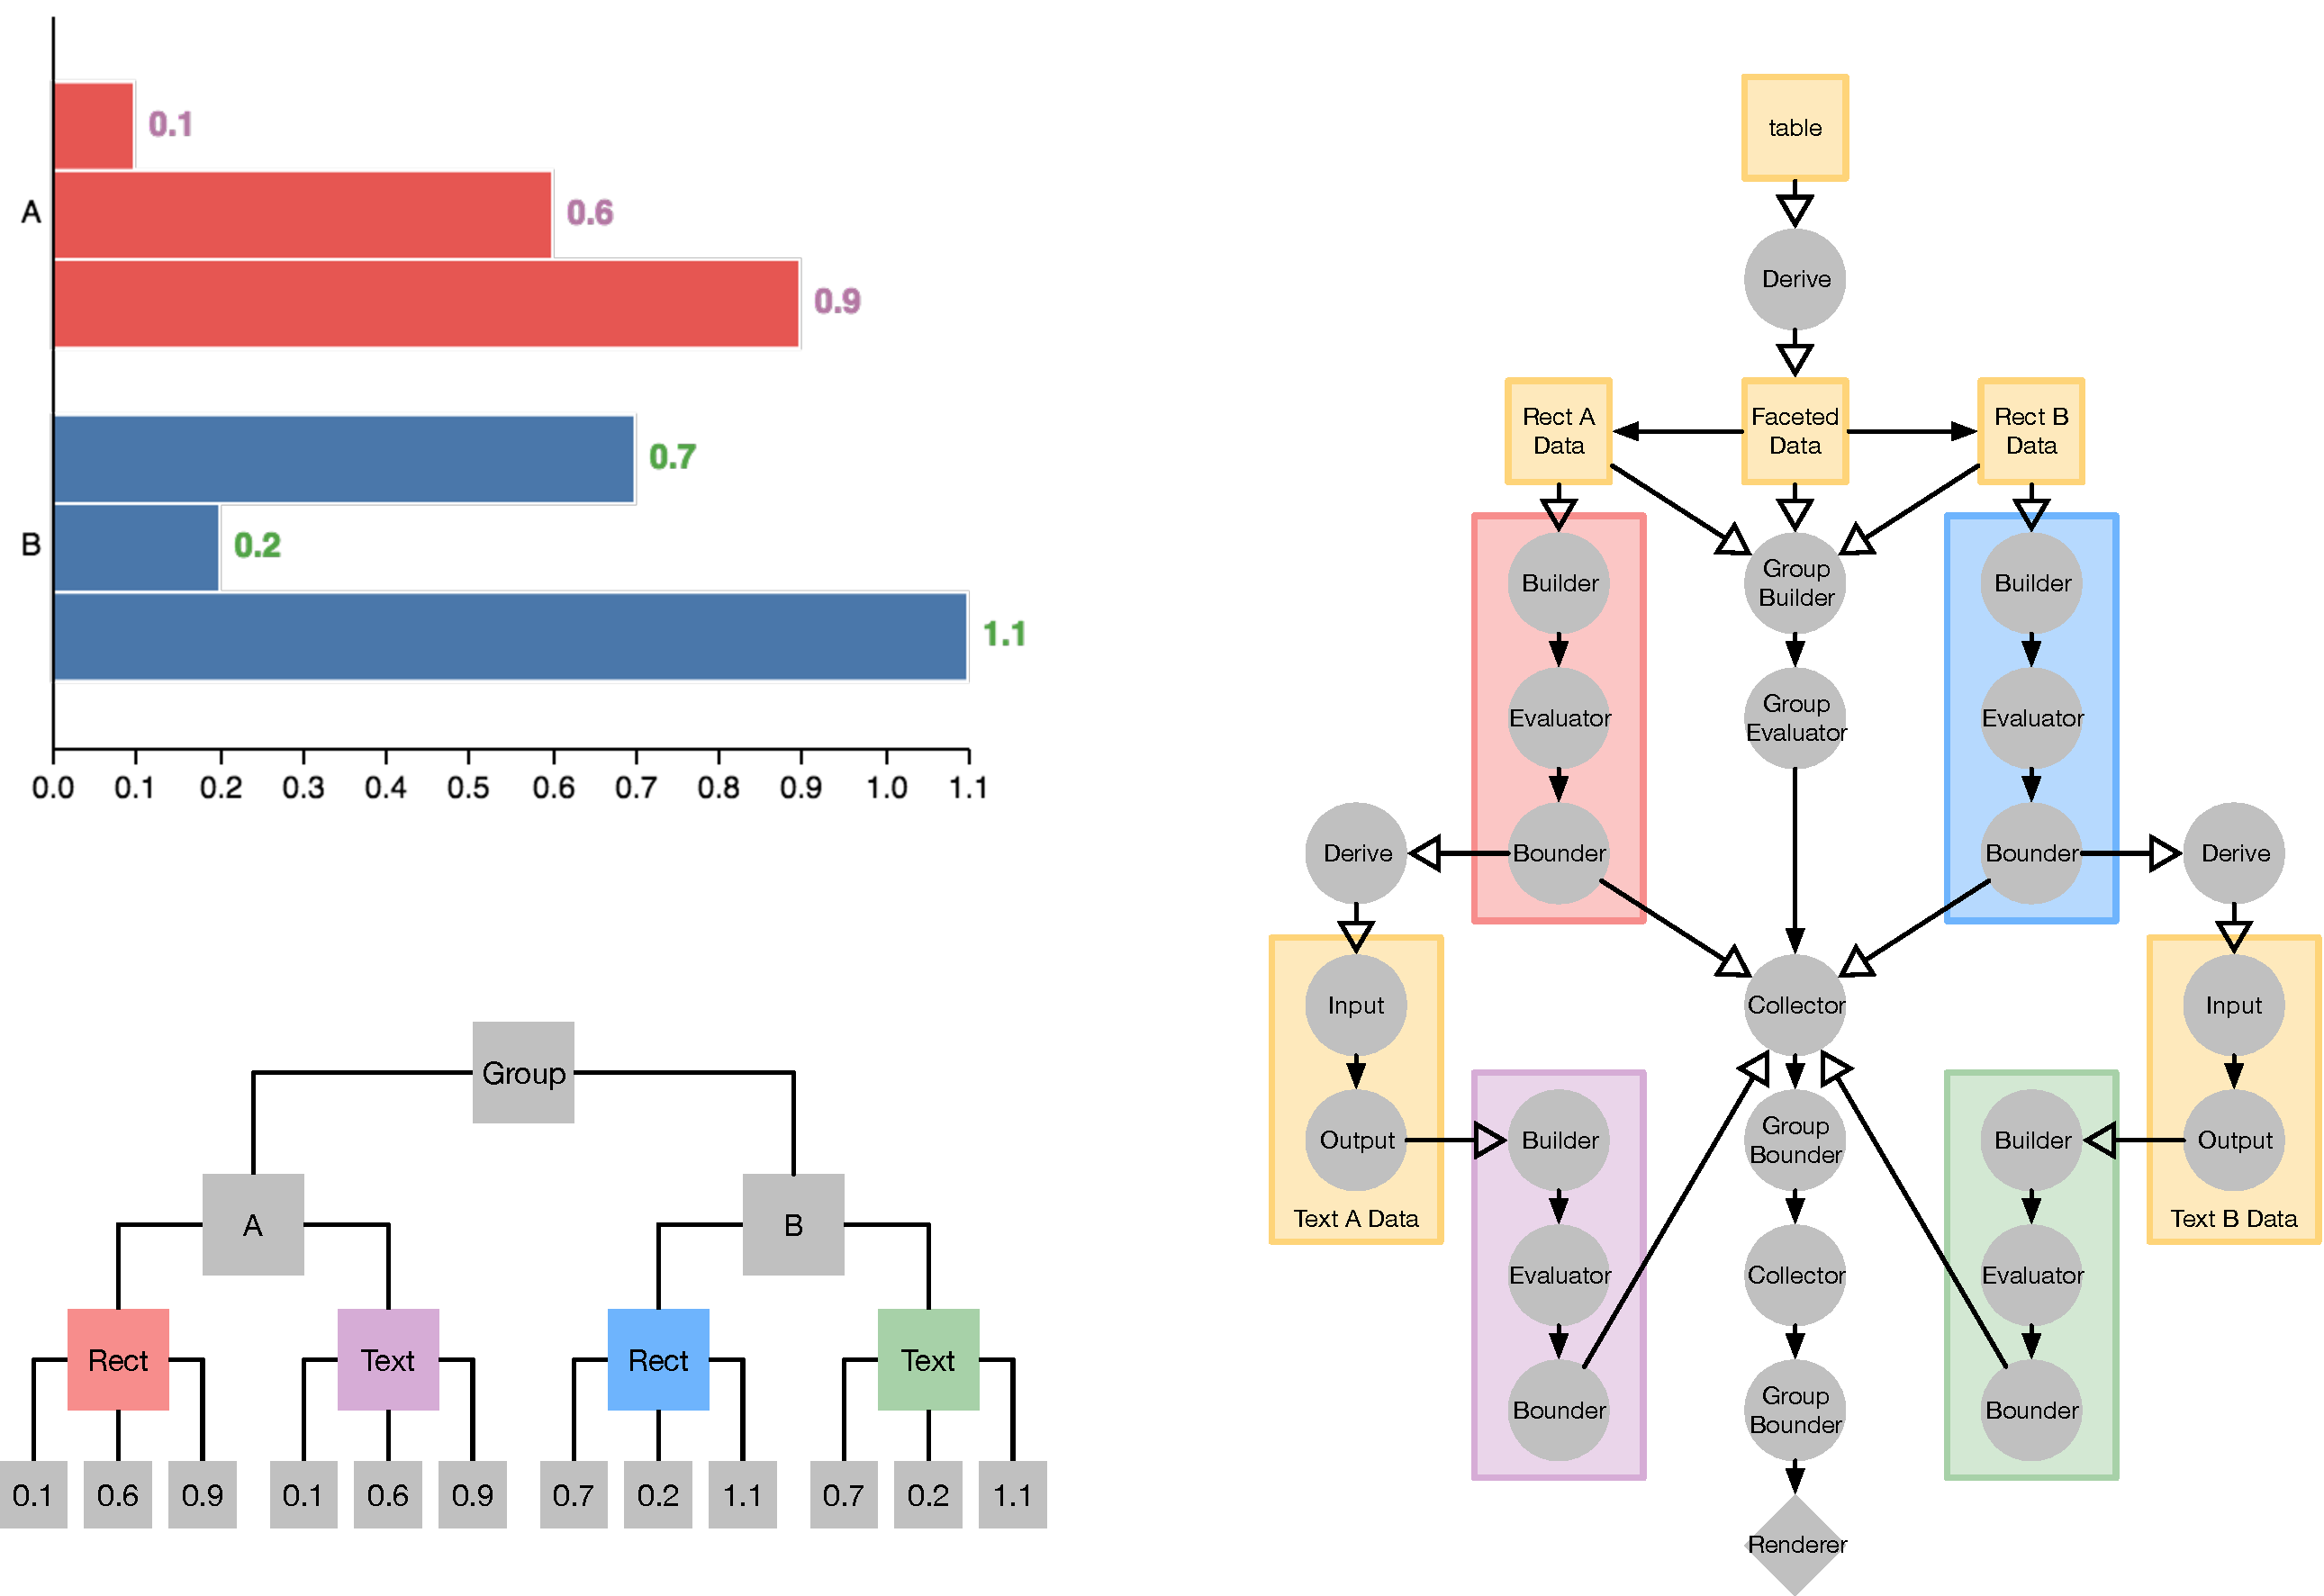
\includegraphics[width=0.9\columnwidth]{groupedBar}
  \caption{A grouped bar chart (top), with the underlying scene graph (bottom),
  and corresponding portion of the dataflow graph (right).}
  \label{fig:vg:groupedBar}
\end{figure}

\begin{figure}[h!]
  \centering
  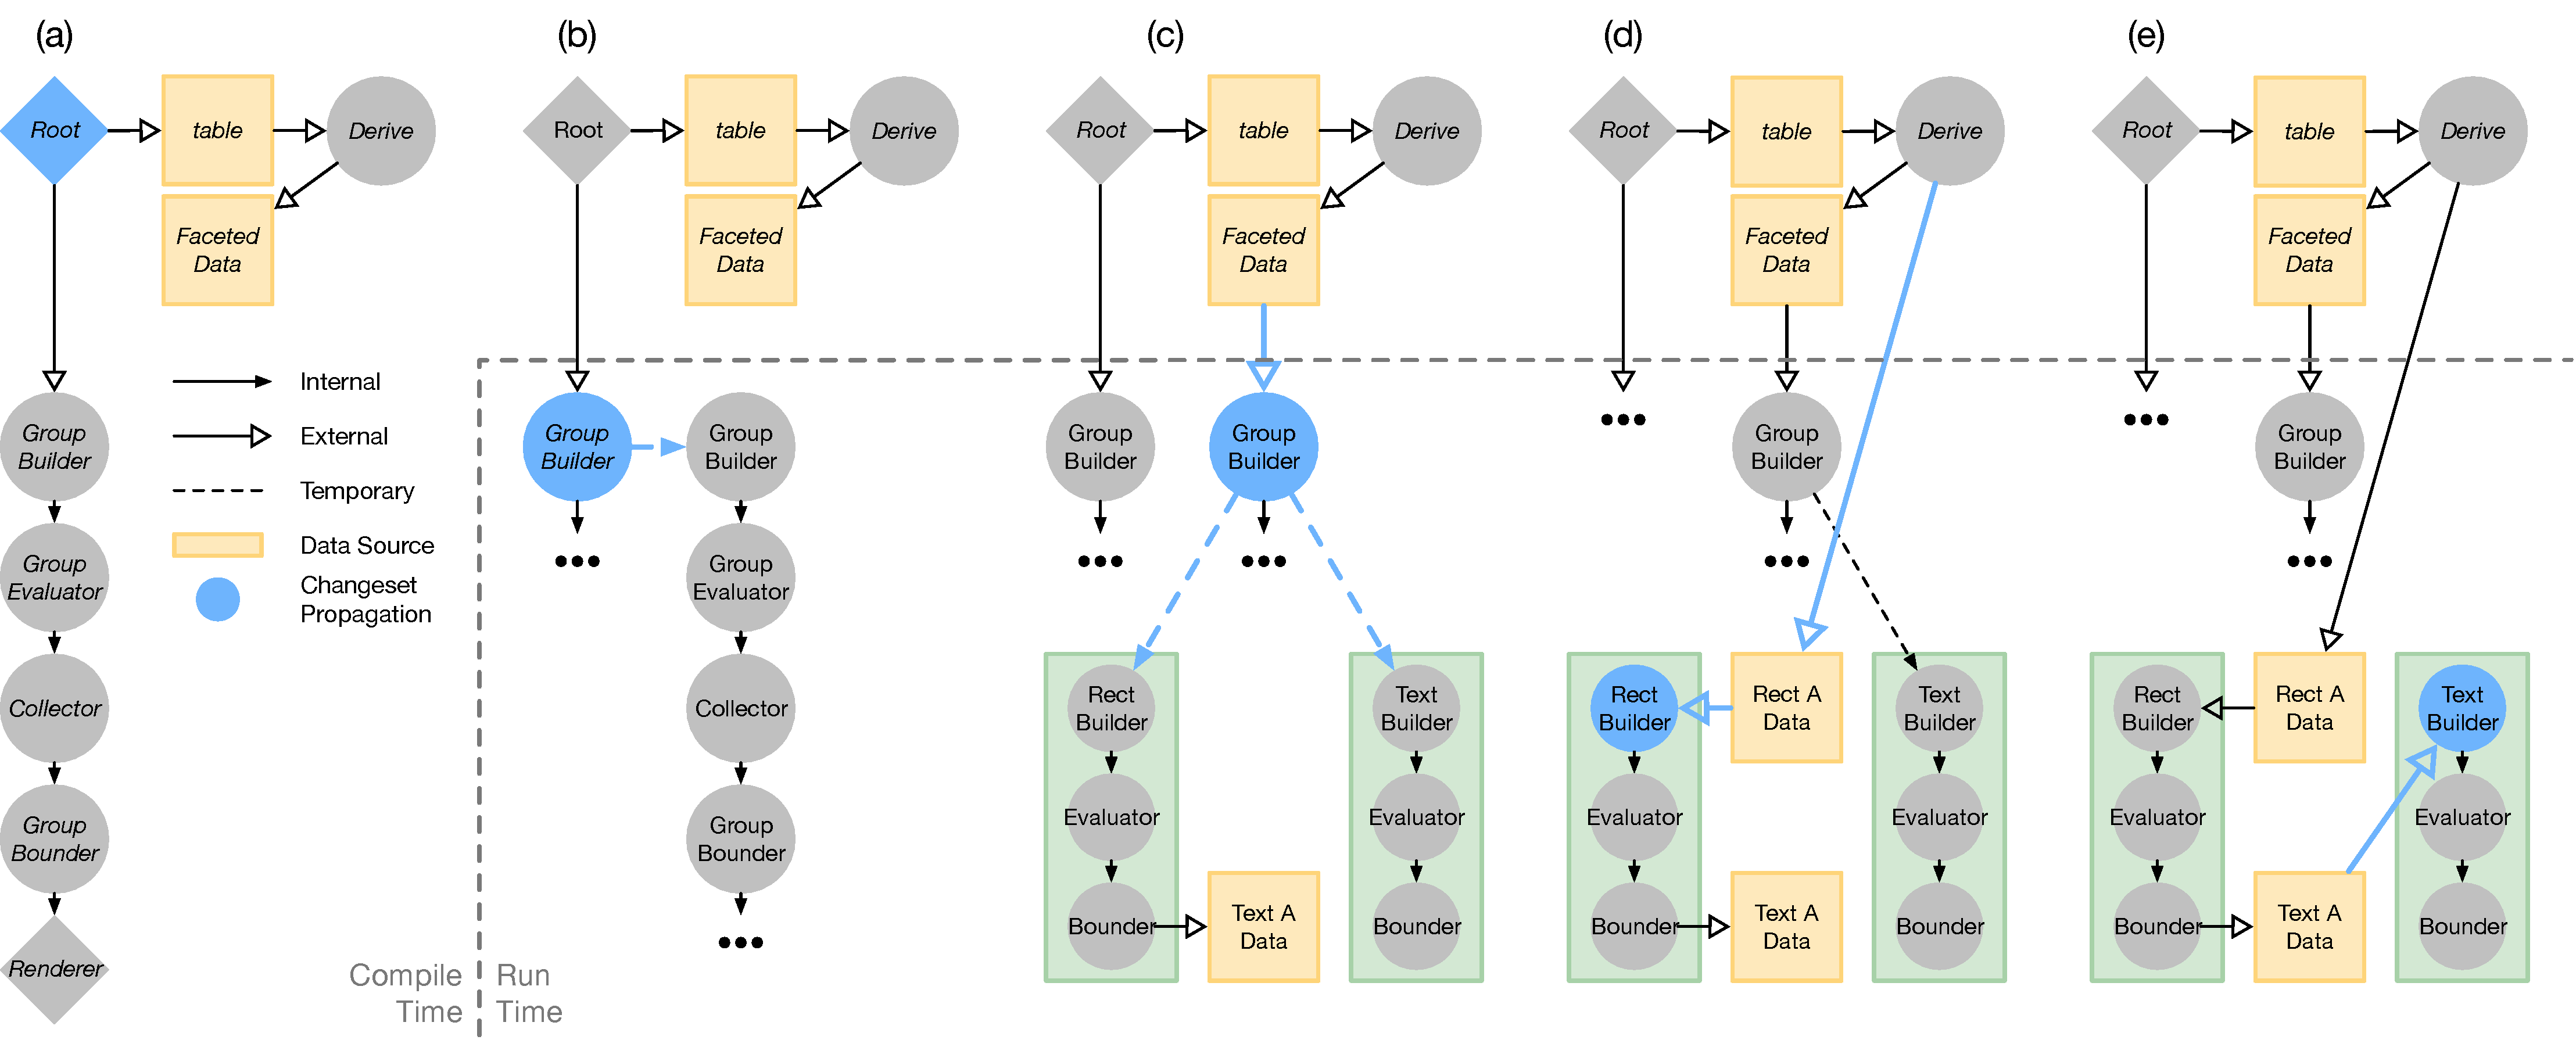
\includegraphics[width=\columnwidth]{scenegraph}
  \caption{Dataflow operators responsible for scene graph construction are
dynamically instantiated at run-time, a process that results in the graph seen
in Fig.~\ref{fig:vg:groupedBar}. (a) At compile-time, a branch corresponding  to
the root scene graph node is instantiated. (b-c) As the changeset (in blue)
propagates through nodes, group-mark builders instantiate builders for their
children. Parent and child builders are temporarily connected (dotted lines) to
ensure children are built in the same timecycle. (d-e) When the changeset
propagates to the children, the temporary connection is replaced with a
connection to the mark's backing data source (also in blue).}
  \label{fig:vg:scenegraph}
\end{figure}

To construct the scene graph, Reactive Vega follows a process akin to the
Protovis bind-build-evaluate pipeline~\cite{heer:protovisjava}. When a
declarative specification is parsed, Reactive Vega traverses the mark hierarchy
to \emph{bind} property definitions: property sets are compiled into encoding
functions and stored with the specification. At run-time, \emph{build} and
\emph{evaluate} operators are created for each bound mark. The build operator
performs a data join~\cite{bostock:d3} to generate one scene graph element (or
``mark'') per tuple in the backing dataset, and the evaluate operator runs the
appropriate encoding functions. A downstream \emph{bounds} operator calculates
the bounding boxes of generated marks. For a nested scene graph to be rendered
correctly, the order of operations is critical: parent marks must be built and
encoded before their children, but the bounds of the children must be calculated
before their parents. The resultant scene graph exhibits an alternating
structure, with individual mark elements grouped under a sentinel mark
specification node. \Cref{fig:vg:scenegraph} illustrates this process for a
grouped bar chart.

Scene graph elements are also modeled as data tuples and can serve as the input
data for downstream visual encoding primitives. This establishes a
\emph{reactive geometry} that accelerates common layout tasks, such as label
positioning, and expands the expressiveness of the specification language. As
marks can be run through subsequent data transformations, higher-level layout
algorithms (e.g., those that require a pre-computed initial
layout~\cite{flexbox}) are now supported in a fully declarative fashion.

\subsection{Changesets and Materialization}

All data does not flow through the system at all times. Instead, operators
receive and transmit \emph{changesets}. A changeset consists of tuples that have
been observed, new signal values, and updates to other dependencies that have
transpired since the last render event. The propagation of a changeset begins in
response to streaming tuples or user interaction. The corresponding input node
creates a fresh changeset, and populates it with the detected update. As the
changeset flows through the graph, operators use it to perform targeted
recomputation, and may augment it in a variety of ways. For example, a
\texttt{Filter} operator might remove tuples from a changeset if they do not
meet the filter predicate, or may mark modified tuples as \texttt{added} if they
previously had been filtered. A Cartesian product operator, on the other hand,
would replace all incoming tuples with the cross-product with another data
stream.

While changesets only include updated data, some operators require a complete
dataset. For example, a windowed-join requires access to all tuples in the
current windows of the joined data sources. For such scenarios, special
\emph{collector} operators (akin to \emph{views}~\cite{abadi:aurora} or
\emph{synopses}~\cite{arasu:stream} in streaming databases) exist to
materialize the data currently in a branch. In order to mitigate the
associated time and memory expenses, Reactive Vega automatically shares
collectors between dependent operators. Upon instatiation, such operators must
be annotated as requiring a collector; at run-time they can then request a
complete dataset from the dataflow graph scheduler.

Finally, if animated transitions are specified, a changeset contains an
interpolation queue to which mark evaluators add generated mark instances; the
interpolators are then run when the changeset is evaluated by the renderer.

\subsection{Coordinating Changeset Propagation}
\label{sec:propagation}

A centralized dataflow graph scheduler is responsible for dispatching changesets
to appropriate operators. The scheduler ensures that changeset propagation
occurs in topological order so that an operator is only evaluated after all of
its dependencies are up-to-date. This schedule prevents wasteful intermediary
computation or momentary inconsistencies, known as
\emph{glitches}~\cite{cooper:embedding}. Centralizing this responsibility,
rather than delegating it to operators, enables more aggressive pruning of
unnecessary computation as described in~\secref{sec:pruning}. The scheduler has
access to the full graph structure and, thus, more insight into the state of
individual operators and propagation progress.

When an interaction event occurs, however, an initial non-topological update of
signals is performed. Dependent signals are reevaluated according to their
specification order. As a result, signals may use prior computed values of their
dependencies, which will subsequently be updated. This process mimics E-FRP's
two-phase update~\cite{wan:efrp}, and is necessary to enable expressive signal
composition. Once all necessary signals have been reevaluated, a changeset with
the new signal values is sent to the scheduler for propagation to the rest of
the dataflow graph.

\subsection{Pushing Internal and Pulling External Changesets}

Two types of edges connect operators in the dataflow graph. The first connects
operators that work with the same data; for example a pipeline of data
transformation operators for the same data source, or a mark's build and
evaluate operators. Changesets are pushed along these edges, and operators
use and augment them directly.

The second type of edge connects operators with external dependencies such as
other data sources, signals, and scale functions. As these edges connect
disparate data spaces, they cannot directly connect operators with their
dependencies. To do otherwise would result in operators performing computation
over mismatched data types. Instead, external dependencies are connected to
their dependents' nearest upstream \texttt{Collector} node, and changesets that
flow along these edges are flagged as \emph{reflow changesets}. When a
\texttt{Collector} receives a reflow changeset, it propagates its tuples
forward, flagging them as modified. The dependents now receive correct input
data and request the latest values of their dependencies from the scheduler.

The only exception to this pattern is when signals rely on other signals.
Reflow changesets still flow along these edges but, as they operate in scalar
data space, they are not mediated by \texttt{Collectors}.

This hybrid push/pull system enables a complex web of interdependent operators
while reducing the complexity of individual elements. For example, regardless of
whether a signal parameterizes data transforms or visual encoding primitives, it
simply needs to output a reflow changeset. Without such a system in place, the
signal would instead have to construct a different changeset for each dependency
edge it was a part of, and determine the correct dataset to supply. \Cref
{fig:vg:teaser,} use
filled and unfilled arrows for internal and external
connections, respectively.

\subsection{Dynamically Restructuring the Graph}

To support streaming nested data structures, operators can dynamically
restructure the graph at runtime by extending new branches, or pruning
existing ones, based on observed data. These dataflow branches model their
corresponding hierarchies as standard relations, thereby enabling subsequent
operators to remain agnostic to higher-level structure. For example, a
\texttt{Facet} operator partitions tuples by key fields; each partition then
propagates down a unique, dynamically-constructed dataflow branch, which can
include other operators such as \texttt{Filter} or \texttt{Sort}.

In order to maintain interactive performance, new branches are queued for
evaluation as part of the same propagation in which they were created. To
ensure changeset propagation continues to occur in topological order,
operators are given a \emph{rank} upon instantiation to uniquely identify
their place in the ordering. When new edges are added to the dataflow graph,
the ranks are updated such that an operator's rank is always greater than
those of its dependencies. When the scheduler queues operators for
propagation, it also stores the ranks it observes. Before propagating a
changeset to an operator, the scheduler compares the operator's current rank
to the stored rank. If the ranks match, the operator is evaluated; if the
ranks do not match, the graph was restructured and the scheduler requeues the
operator.

The most common source of restructuring operations are scene graph operators, as
building a nested scene graph is entirely data-driven. Dataflow branches for
child marks (consisting of build-evaluate-bound chains) cannot be instantiated
until the parent mark instances have been generated. As a result, only a single
branch, corresponding to the root node of the scene graph, is constructed at
compile-time. As data streams through the graph, or as interaction events occur,
additional branches are created to build and encode corresponding nested marks.
To ensure their marks are rendered in the same propagation cycle, new branches
are temporarily connected to their parents. These connections are subsequently
removed so that children marks will only be rebuilt and re-encoded when their
backing data source updates. Figure~\ref{fig:vg:scenegraph} provides a
step-by-step illustration of how scene graph operators are constructed during a
propagation cycle for the grouped bar chart in Figure~\ref{fig:vg:groupedBar}.
% !TEX root = ../thesis.tex
\section{Performance Optimizations}
\label{sec:vg:optimizations}

Declarative language runtimes can transparently optimize
performance~\cite{heer:protovisjava} and Reactive Vega uses several strategies
to increase throughput and reduce memory usage. In this section, we describe
these strategies and evaluate their effect through benchmark studies. Each
benchmark was run with datasets sized at N = 100, 1,000, 10,000, and 100,000
tuples. For ecological validity, benchmarks were run with Google Chrome 42
(64-bit) and, to prevent confounds with browser-based just-in-time (JIT)
optimizations, each iteration was run in a fresh instance. All tests were
conducted on a MacBook Pro system running Mac OS X 10.10.2, with a quad-core
2.5GHz Intel Core i7 processor and 16GB of 1600 MHz DDR3 RAM.

\subsection{On-Demand Tuple Revision Tracking}

\begin{figure}[h!]
  \centering
  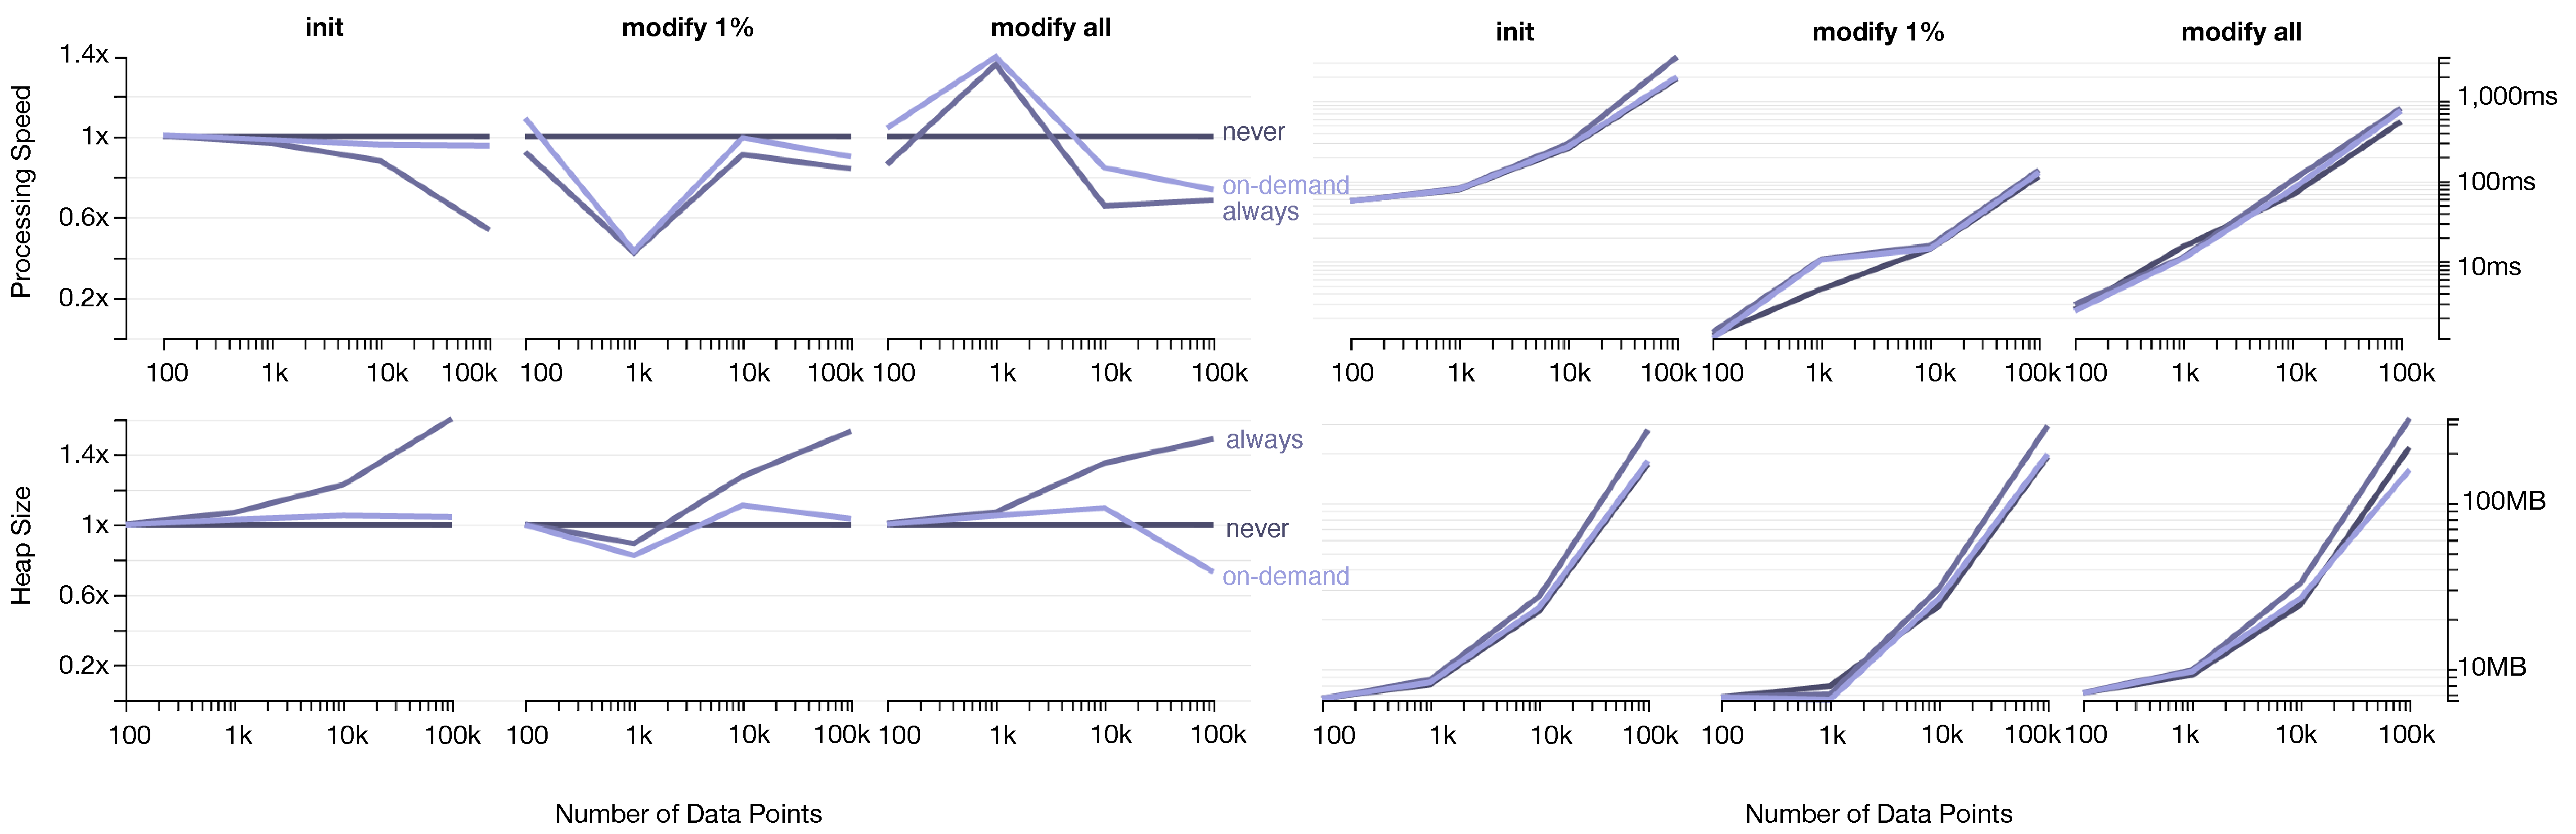
\includegraphics[width=\columnwidth]{prev-lines.pdf}
  \caption{Effects of tuple revision optimizations on average
processing speed (top) and memory footprint (bottom). Left-hand figures show
relative changes using no-tracking as a baseline (closer to 1.0 are better),
and right-hand figures show the absolute values on a log$_{10}$ scale
(lower is better).}
  \label{fig:vg:prev_benchmark}
\end{figure}

Some operators (e.g., statistical aggregates) require both a tuple's current and
previous values. Tracking prior values can affect both running time and memory
consumption. One strategy to minimize this cost is to track tuple revisions only
when necessary. Operators must declare their need for prior values. Then, when
tuples are ingested, their previous values are only tracked if the scheduler
determines that they will flow through an operator that requires revision
tracking.

We ran a benchmark comparing three conditions: always track revisions, never
track revisions, and on-demand tracking. Although the ``never'' condition
produces incorrect results, it provides a lower-bound for performance. We
measured the system's throughput as well as memory allocated when initializing a
scatterplot specification, and after modifying either 1\% or 100\% of input
tuples. The scatterplot features two symbol marks fed by two distinct dataflows,
\texttt{A} and \texttt{B}. Both branches ingest the same set of tuples, and
include operators that derive new attributes. However, \texttt{B} includes
additional aggregation operators that require revision tracking.

The results are shown in Figure~\ref{fig:vg:prev_benchmark}, with the effects of
revision tracking most salient at larger dataset sizes. Always tracking
revisions can require 20-40\% more memory, and can take up to 50\% longer to
initialize a visualization due to object instantiation overhead for storing
previous values. Our on-demand strategy effectively reduces these costs,
requiring only 5-10\% more memory and taking 5\% longer to initialize than the
``never'' condition.

\subsection{Pruning Unnecessary Recomputation}
\label{sec:pruning}

\begin{figure}[h!]
  \centering
  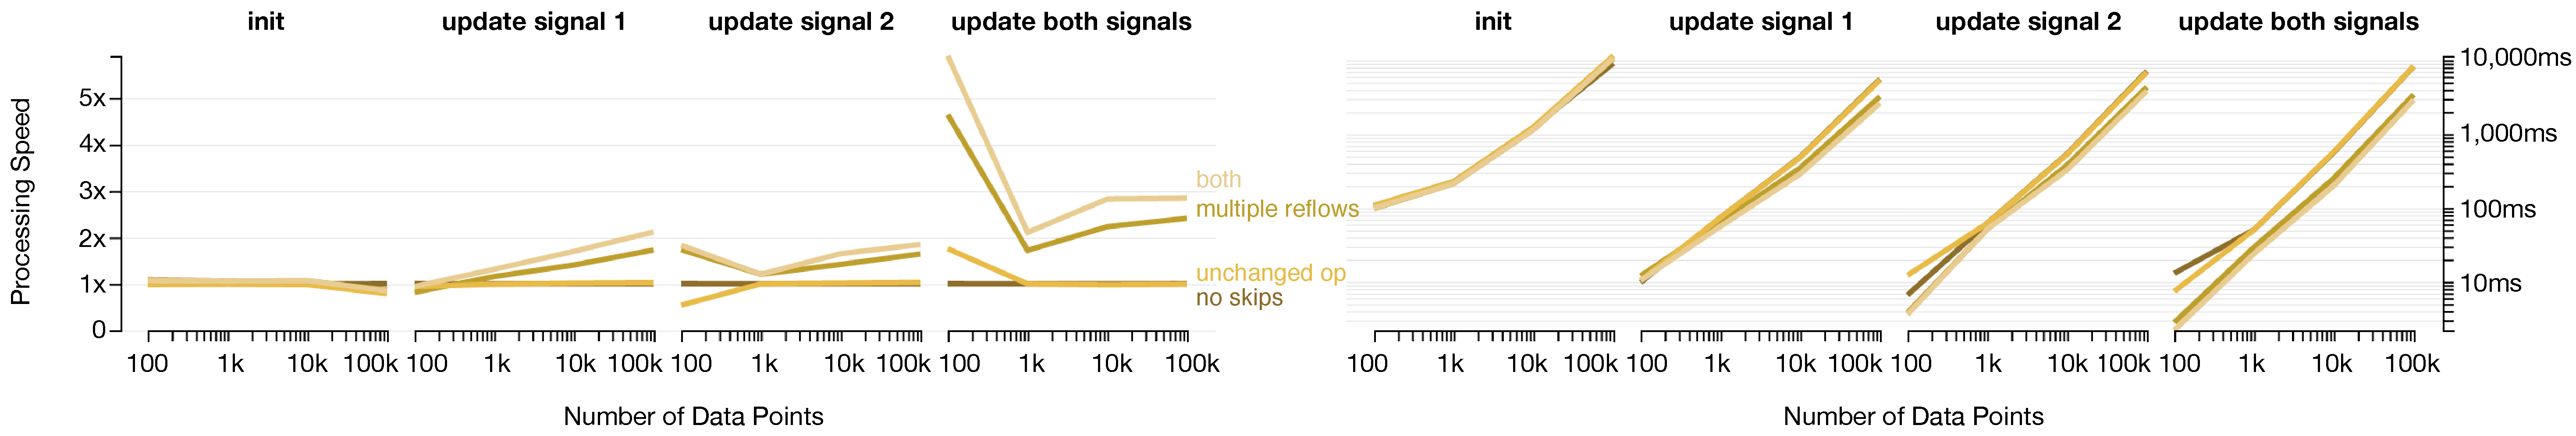
\includegraphics[width=\columnwidth]{skips-lines.pdf}
  \caption{The effects of pruning unnecessary computation on average processing
speed. (a) A relative difference between conditions (higher is better). (b)
Absolute values for time taken, plotted on a log$_{10}$ scale (lower is better).}
  \label{fig:vg:skips_benchmark}
\end{figure}

By centralizing responsibility for operator scheduling and changeset dispatch,
we can aggressively prune unnecessary recomputation. The dataflow graph
scheduler knows the current state of the propagation, and dependency
requirements for each queued operator, allowing us to perform two types of
optimizations:

\begin{enumerate}
  \item \emph{Pruning multiple reflows of the same branch}. As the scheduler
  ensures a topological propagation ordering, a branch can be safely pruned for
  the current propagation if it has already been reflowed.

  \item \emph{Skipping unchanged operators}. Operators identify their
dependencies\,---\,including signals, data fields, and scale functions\,---\,and
changesets maintain a tally of updated dependencies as they flow through the
graph. The scheduler skips evaluation of an individual operator if it is not
responsible for deriving new tuples, or if a changeset contains only modified
tuples and no dependencies have been updated. Downstream operators are still
queued for propagation.
\end{enumerate}

To measure the impact of these optimizations, we created a grouped bar chart
with five data transformation operators: \texttt{Derive(signal1)} $\rightarrow$
\texttt{Fold} $\rightarrow$ \texttt{Derive(signal2)} $\rightarrow$
\texttt{Filter (signal2)} $\rightarrow$ \texttt{Facet}.  We then benchmarked the
effect of four conditions (processing all recomputations, pruning multiple
reflows only, skipping unchanged operators only, and applying both
optimizations) across four tasks (initializing the visualization, updating each
signal in turn, and updating both signals together).

Results are shown in Figure~\ref{fig:vg:skips_benchmark}. Preventing multiple
reflows is the most effective strategy, increasing throughput 1.4 times on
average. Skipping unchanged operators sees little benefit by itself as, in our
benchmark setup, only the two operators following a fold are skipped when
changing \texttt{signal1}, and only the first derivation operator is skipped
when changing \texttt{signal2}. When the two strategies are combined, however,
we see a 1.6x increase in performance. This result was consistent across
multiple benchmark trials. After careful hand-verification to ensure no
additional nodes were erroneously skipped, we hypothesize that the JavaScript
runtime is able to perform just-in-time optimizations that it is unable to apply
to the other conditions.

\subsection{Inlining Sequential Operators}

\begin{figure}[h!]
  \centering
  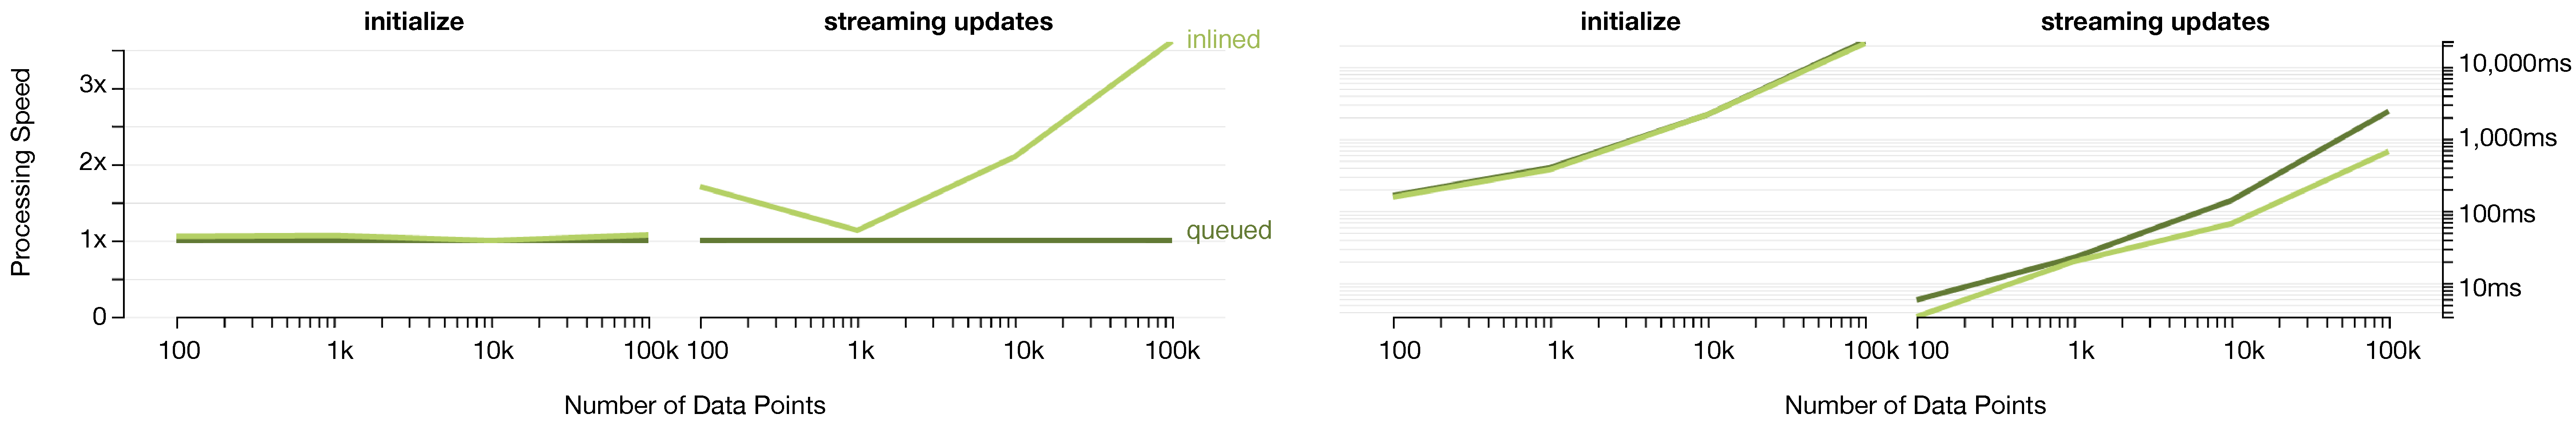
\includegraphics[width=\columnwidth]{inlined-lines.pdf}
  \caption{The effects of inlining sequential operators on average processing
speed. (a) A relative difference between conditions (higher is better). (b)
Absolute values for time taken, plotted on a log$_{10}$ scale (lower is better).}
  \label{fig:vg:inline_benchmark}
\end{figure}

To propagate changesets through the dataflow graph, the scheduler adds operators
to a priority queue, backed by a binary heap sorted in topological order. This
incurs an $O(log N)$ cost for enqueueing and dequeueing operators, which can be
assessed multiple times per operator if the graph is dynamically restructured.
However, branching only occurs when operators register dependencies, and
dependencies are only connected to \texttt{Collector} nodes. As a result, much
of the dataflow graph comprises linear paths. This is particularly true for
scene graph operators, which are grouped into hundreds (or even thousands) of
independent mark build-evaluate-bound branches.

We explore the effect of inline evaluation of linear branches, whereby operators
indicate that their neighbors can be called directly rather than queued for
evaluation. The scheduler remains responsible for propagating the changeset,
and thus can continue to apply the optimizations previously discussed. Although
inline evaluation can be applied in a general fashion by coalescing linear
branches into ``super nodes,'' for simplicity we only evaluate inlining of scene
graph operators here. Mark builders directly call evaluators and bounders, and
group mark builders directly call new child mark builders rather than forming a
temporary connection.

Figure~\ref{fig:vg:inline_benchmark} shows the results of this optimization
applied to a parallel coordinates plot. The plot uses a nested scene graph in
which each line segment is built by a dedicated build-evaluate-bound branch. As
we can see, inlining does not have much impact on the initialization time. This
is unsurprising, as the largest initialization cost is due to unavoidable graph
restructuring. However, inlining improves streaming operations by a 1.9x factor
on average. As streaming updates only propagate down specific branches of the
dataflow graph, inline evaluation results in at least 4 fewer queuing operations
by the scheduler.
% !TEX root = ../thesis.tex

\vspace{-20pt}

\section{Comparative Performance Benchmarks}
\label{sec:vg:performance}

\vspace{-10pt}

To evaluate the performance of Reactive Vega against D3~\cite{bostock:d3} and
the origin, non-reactive Vega system (v1.5.0), we use the same setup described
in the previous section.

\vspace{-10pt}

\subsection{Streaming Visualizations}

\vspace{-7pt}

Figure~\ref{fig:vg:static_benchmark} shows the average performance of
uninteractive streaming scatter plots, parallel coordinates plots, and trellis
plots. We first measured the average time to initially parse and render the
visualizations. To gauge streaming performance, we next measured the average
time taken to update and re-render upon adding, modifying, or removing 1\% of
tuples. We ran 10 trials per dataset, sized 100--100,000 tuples.

\begin{figure}[t!]
  \centering
  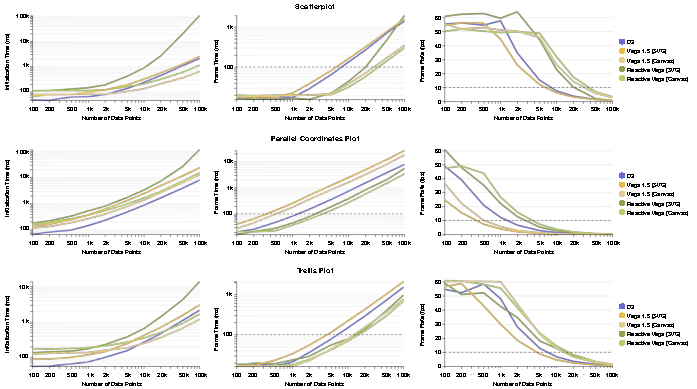
\includegraphics[width=\columnwidth]{streaming-lines.pdf}
  \caption{Average performance of rendering (non-interactive) streaming visualizations:
(top-bottom) scatterplot, parallel coordinates, and trellis plot; (left-right)
initialization time, average frame time, and average frame rate. Dashed lines
indicate the threshold of interactive updates~\cite{card:modelhuman}.}
  \label{fig:vg:static_benchmark}
\end{figure}

Reactive Vega has the greatest effect with the parallel coordinates plot,
displaying 2x and 4x performance increases over D3 and Vega 1.5, respectively.
This effect is due to each plotted line being built and encoded by its own
dataflow branch. Across the other two examples, and averaging between the Canvas
and SVG renderers, we find that although Reactive Vega takes 1.7x longer to
initialize the visualizations, subsequent streaming operations are 1.9x faster
than D3. Against Vega 1.5, Reactive Vega is again 1.7x slower at initializing
visualizations; streaming updates perform roughly op-par with the Canvas
renderer, but are 2x faster with the SVG renderer.

Slower initialization times for Reactive Vega are to be expected. D3 does not
have to parse and compile a JSON specification, and a streaming dataflow graph
is a more complex execution model, with higher overheads, than batch processing.
However, with streaming visualizations this cost amortizes and performance in
response to data changes becomes more important. In this case, Reactive Vega
makes up the difference in a single cycle.

\vspace{-10pt}

\subsection{Interactive Visualizations}

\vspace{-7pt}

We evaluated the performance of interactive visualizations (measured in terms of
interactive frame rate) using three common examples: brushing \& linking a
scatterplot matrix, a time-series overview+detail visualization, and panning \&
zooming a scatterplot. We chose these examples as they all leverage interactive
behaviors supported by D3, with canonical implementations available for
each\footnote{Brushing \& Linking:
http://bl.ocks.org/mbostock/4063663}\textsuperscript{,}\footnote{Overview +
Detail: http://bl.ocks.org/mbostock/1667367}\textsuperscript{,}\footnote{Pan \&
Zoom: http://bl.ocks.org/mbostock/3892919}. For Reactive Vega, we expressed
these visualizations with a single declarative specification. For D3 and Vega
1.5, we use custom event handling callbacks. The Vega 1.5 callbacks mimic the
behavior of the fragmented reactive approach used in prior
work~\cite{satyanarayan:declarative}. We tested these visualizations with
datasets sized between 100 and 10,000 tuples.

\begin{figure}[t!]
  \centering
  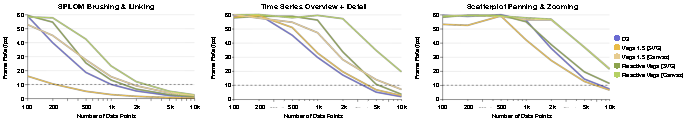
\includegraphics[width=\columnwidth]{interaction-lines.pdf}
  \caption{Average frame rates for three interactive visualizations: (left-right)
  brushing and linking on a scatterplot matrix; brushing and linking on an
  overview+detail visualization; panning and zooming on a scatterplot. Dashed
  lines indicate the threshold of interactive updates~\cite{card:modelhuman}.}
  \label{fig:vg:interactive_benchmark}
\end{figure}

Figure~\ref{fig:vg:interactive_benchmark} shows the results\,---\,on average,
and across both Canvas and SVG renderers, Reactive Vega offers superior
interactive performance to custom D3 and Vega event handling callbacks. This
effect primarily stems from Reactive Vega's unified data model, and is most
noticeable with brushing \& linking a scatterplot matrix and the time-series
overview+detail visualization. In both examples, interactions manipulate only a
subset of all data tuples. With Reactive Vega, only these tuples are processed,
and their corresponding scene graph elements re-encoded and re-rendered. In
contrast, Vega 1.5's fragmented reactive approach reconstructs and re-renders
the entire scene graph in response to changing data.
% !TEX root = ../thesis.tex
\section{Conclusion \& Future Work}
\label{sec:vg:conclusion}

Declarative languages are a popular means of authoring
visualizations~\cite{bostock:protovis, bostock:d3, heer:protovisjava}, but have
lacked first-class support for interaction design. In response, we contribute
Reactive Vega, the first language and system architecture to support declarative
visualization and interaction design in a comprehensive and performant fashion.

It is important to note that although Reactive Vega provides an complete
end\--to\--end system\,---\,whereby users invoke the parser to traverse an
input declarative specification and instantiate the necessary architecture
components to render a visualization\,---\,this process can be decoupled.
Reactive Vega's declarative model can be used to implement extensions to D3, and
higher-level tools can opt to manually construct and connect required dataflow
operators.

By simplifying programmatic generation of visualization, Reactive Vega's
declarative JSON syntax has led to a growing ecosystem of higher-level
visualization systems. For example, MapD~\cite{mapd:vega} has integrated Vega
with their GPU-powered database; custom SQL queries can be embedded within the
JSON specification, which is dispatched to the backend server, rendered, and
returned to the client as a PNG image. Similarly, Wikipedia, a security-concious
environment where it would be difficult to allow users to write imperative
visualization code, has recently integrated Vega~\cite{mediawiki:graph} to
enable visualization of data embedded in articles.

Still, improved support for authoring and debugging Vega specifications remains
a promising avenue for future work. In recent work, Hoffswell
et~al.~\cite{hoffswell:debugging} developed a ``time-traveling'' debugger for
Reactive Vega specifications and found that first-time Vega users were able to
accurately trace errors through the specification. Further work, particularly by
instrumenting Reactive Vega's dataflow graph to enable inspection and stepping
through changeset propagation could aid in learnability~\cite{guo:tutor}.
Through the development of such tools, we can also assess the accessibility of
the language. Are new users able to learn the declarative interaction model? Can
experts, accustomed to callback-driven programming, quickly transition as well?

Reactive Vega's architecture also offers opportunities to study scalable
visualization design. Interactive visualization of large-scale datasets often
requires offloading computation to server-side architectures. For example,
Nanocubes~\cite{lins:nanocubes} and imMens~\cite{liu:immens} assemble
multi\--dimensional data cubes that can be decomposed into smaller data tiles
and pushed to the client. Such components could be integrated into a dataflow
graph with execution distributed across server and client~\cite{domoritz:dsia}.
For example, as the dataflow graph scheduler is responsible for propagation, it
might anticipate possible user interactions and prefetch data tiles in order to
reduce latency~\cite{battle:prefetch}.

Reactive Vega is an open source system available at
\url{http://vega.github.io/vega/}.
% !TEX root = ../thesis.tex
\graphicspath{{./vega-lite/figures/}}
\chapter{A Grammar of Interactive Graphics}

\begin{figure}[h!]
  \vspace{-30pt}
  \centering
  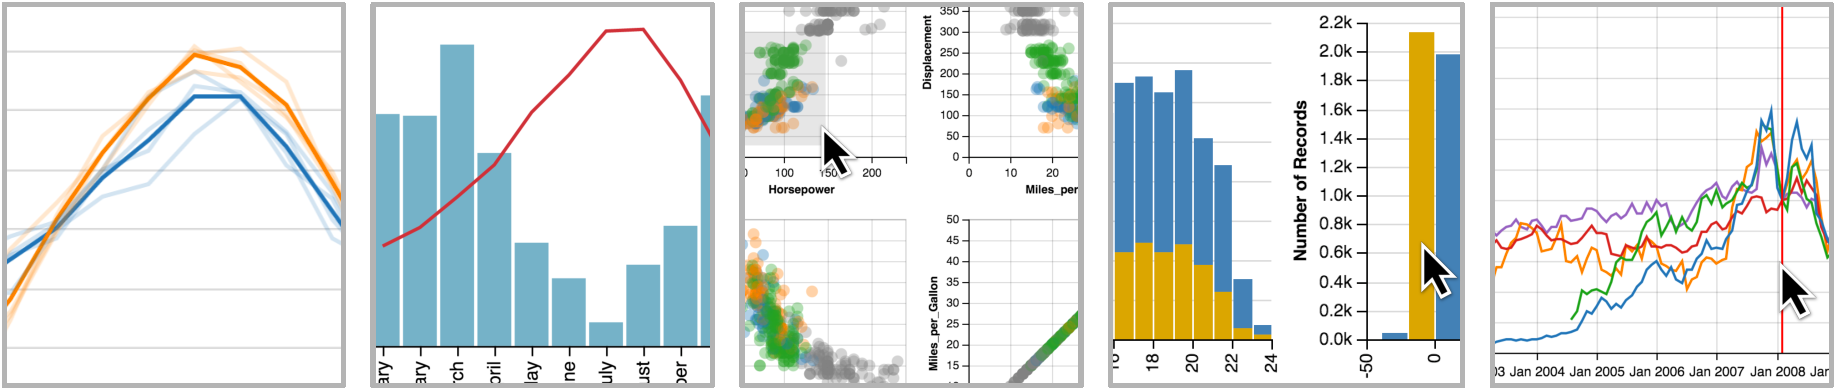
\includegraphics[width=\columnwidth]{teaser}
  % \vspace{-30pt}
\end{figure}

% Reactive Vega demonstrates that the advantages of declarative specification
% extend to interaction design as well\,---\,decoupling specification from
% execution frees designers to iterate more quickly, facilitates retargeting
% across platforms, and allows for language-level optimizations.

Reactive Vega demonstrates that declarative interaction design is an expressive
and performant alternative to imperative event handling callbacks. However, as
its abstractions are relatively low-level, it would be apt to describe it as an
``assembly language'' for interactive visualization most suited for
\emph{explanatory} visualization. In contrast, for \emph{exploratory}
visualization, higher-level grammars such as ggplot2~\cite{wickham:layered}, and
grammar-based systems such as Tableau (n\'ee Polaris~\cite{stolte:polaris}), are
typically preferred as they favor conciseness over expressiveness. Analysts
rapidly author partial specifications of visualizations; the grammar applies
default values to resolve ambiguities, and synthesizes low-level details to
produce visualizations.

High-level languages can also enable search and inference over the space of
visualizations. For example, Wongsuphasawat et~al. introduced Vega-Lite to power
the Voyager visualization browser~\cite{voyager}. By providing a smaller surface
area than Vega, Vega-Lite makes systematic enumeration and ranking of data
transformations and visual encodings more tractable.

However, existing high-level languages provide limited support for
interactivity. An analyst can, at most, enable a predefined set of common
techniques (linked selections, panning \& zooming, etc.) or parameterize their
visualization with dynamic query widgets~\cite{shiny}. For custom,
direct-manipulation interaction they must, once again, turn to imperative event
handling callbacks.

In this chapter, we extend Vega-Lite with a \emph{multi-view} grammar of
graphics alongside a novel \emph{grammar of interaction} to enable concise,
high-level specification of interactive data visualizations.

% !TEX root = ../thesis.tex
\section{Visual Encoding}
\label{sec:vlgog}

The simplest Vega-Lite specification\,---\,referred to as a \emph{unit}
specification\,---\,describes a single Cartesian plot with the following
four-tuple:

\signaturevspace
\centerline{\emph{unit := (data, transforms, mark-type, encodings)}}
\signaturevspace

The \emph{data} definition identifies a data source, a relational table
consisting of records (rows) with named attributes (columns). This data table
can be subject to a set of \emph{transforms}, including filtering and adding
derived fields via formulas. The \emph{mark-type} specifies the geometric object
used to visually encode the data records. Legal values include \emph{bar},
\emph{line}, \emph{area}, \emph{text}, \emph{rule} for reference lines, and
plotting symbols (\emph{point} \& \emph{tick}). The \emph{encodings} determine
how data attributes map to the properties of visual marks. Formally, an encoding
is a seven-tuple:

\signaturevspace
\centerline{\emph{encoding := (channel, field, data-type, value, functions, scale, guide)}}
\signaturevspace

Available visual encoding \emph{channels} include spatial position (\emph{x},
\emph{y}), \emph{color}, \emph{shape}, \emph{size}, and \emph{text}. An
\emph{order} channel controls sorting of stacked elements (e.g., for stacked bar
charts and the layering order of line charts). A \emph{path} order channel
determines the sequence in which points of a line or area mark are connected to
each other. A \emph{detail} channel includes additional group-by fields in
aggregate plots.

The \emph{field} string denotes a data attribute to visualize, along with a
given \emph{data-type} (one of \emph{nominal}, \emph{ordinal}, \emph{quantitative} or
\emph{temporal}). Alternatively, one can specify a constant literal \emph{value}
to serve as the data field. The data field can be further transformed using
\emph{functions} such as binning, aggregation (e.g., mean), and sorting.

An encoding may also specify properties of a \emph{scale} that maps from the
data domain to a visual range, and a \emph{guide} (axis or legend) for
visualizing the scale. If not specified, Vega-Lite will automatically populate
default properties based on the \emph{channel} and \emph{data-type}. For \emph
{x} and \emph{y} channels, either a linear scale (for quantitative data) or an
ordinal scale (for ordinal and nominal data) is instantiated, along with an
axis. For \emph{color}, \emph{size}, and \emph{shape} channels, suitable
palettes and legends are generated. For example, quantitative color encodings
use a single-hue luminance ramp, while nominal color encodings use a categorical
palette with varied hues. Our default assignments largely follow the model of
prior systems~\cite{stolte:polaris, voyager}.

Unit specifications are capable of expressing a variety of common, useful plots
of both raw and aggregated data. Examples include bar charts, histograms, dot
plots, scatter plots, line graphs, and area graphs. Our formal definitions are
instantiated in a JSON (JavaScript Object Notation) syntax, as shown in
% \fig{Units}.

\section{View Composition Algebra}

Multiple \emph{unit} specifications can be composed using the following
operators:

\begin{itemize}
  \item \emph{layer([$unit_1$, $unit_2$, ...], resolve)} produces a view in
  which subsequent charts are plotted on top of each other. To produce coherent
  and comparable layers, we share scales (if their types match) and merge guides
  by default. For example, we compute the union of the data domains for the
  \emph{x} or \emph{y} channel, for which we then generate a single scale.
  However, Vega-Lite can not enforce that a unioned domain is
  \emph{semantically} meaningful. To prohibit layering of composite views with
  incongruent internal structures, the \emph{layer} operator restricts its
  operands to be \emph{unit} views.

  \item \emph{hconcat([$view_1$, $view_2$, ...], resolve)} and
  \emph{vconcat([$view_1$, $view_2$, ...], resolve)} place views side-by-side
  horizontally or vertically, respectively. If aligned spatial channels have
  matching data fields (e.g., the \emph{y} channels in an \emph{hconcat} use the
  same field), a shared scale and axis are used. Axis composition facilitates
  comparison across views and optimizes the underlying implementation.

  \item \emph{facet(data, field, view, channel, scale, axis, resolve)} produces
  a trellis plot~\cite{becker:trellis} by subsetting the \emph{data} by the
  distinct values of a \emph{field}. The \emph{view} specification provides a
  template for the sub-plots, and inherits the backing \emph{data} for each
  partition from the operator. The \emph{channel} indicates if sub-plots should
  be laid out vertically (\emph{row}) or horizontally (\emph{column}), and the
  \emph{scale} and \emph{axis} parameters enable further customization of
  sub-plot layout and labeling.

    To facilitate comparison, scales and guides for quantitative fields are shared
  by default. This ensures that each facet visualizes the same data domain.
  However, for ordinal scales we generate independent scales by default to avoid
  unnecessary inclusion of empty categories, akin to Polaris' \emph{nest}
  operator. When faceting by fiscal quarter and visualizing per-month data in each
  cell, one likely wishes to see three months per quarter, not twelve months of
  which nine are empty.

  \item \emph{repeat(values, view, channel, scale, axis, resolve)} generates
  one plot for each entry in a list of \emph{values}. The \emph{view}
  specification provides a template for the sub-plots, and inherits the full
  backing dataset. Encodings within the repeated \emph{view} specification can
  refer to this provided \emph{value} to parameterize the plot\footnote{As the
  \emph{repeat} operator requires parameterization of the inner view, it is not
  strictly algebraic. It is possible to achieve algebraic ``purity'' via
  explicit repeated concatenation or by reformulating the repeat operator (e.g.,
  by including rewrite rules that apply to the inner view specification).
  However, we believe the current syntax to be more usable and concise than
  these alternatives.}. As with \emph{facet}, the \emph{channel} indicates if
  plots should divide by \emph{row} or \emph{column}, with further customization
  possible via the \emph{scale} and \emph{axis} components. By default, scales
  and axes are independent, but legends are shared when data fields coincide.
\end{itemize}

Each operator provides default strategies to \emph{resolve} scales, axes, and
legends across views, as described above. A user can choose to override these
default behaviours by specifying tuples of the form \emph{(channel,
scale$|$axis$|$legend, union$|$independent)}.

These operators form an algebra: the output of one operator can serve as input
to a subsequent operator. As a result, complex nested views and dashboards can
be concisely specified. For instance, a layer of two unit views might be
repeated, and then concatenated with a different unit view. The one exception is
the \emph{layer} operator, which, as previously noted, only accepts unit views
to ensure consistent plots. For concision, two dimensional faceted or repeated
layouts can be achieved by applying the operators to the \emph{row} and
\emph{column} channels simultaneously. When faceting a composite view, only the
dataset targeted by the operator is partitioned; any other datasets specified in
sub-views are replicated.
% !TEX root = ../thesis.tex
\section{Interactive Selections}
\label{sec:vlgoi}

To support specification of interaction techniques, we extend the definition of
unit specifications to also include a set of \emph{selections}. Selections
identify the set of points a user is interested in manipulating, and is formally
defined as an eight-tuple:

\centerline{
  \emph{selection := (name, type, predicate, domain$|$range, event, init,
  transforms, resolve})
}

When an input \emph{event} occurs, the selection is populated with \emph{backing
points} of interest. These points are the minimal set needed to identify all
\emph{selected points}. The selection \emph{type} determines how many backing
values are stored, and how the \emph{predicate} function uses them to determine
the set of selected points. Supported types include a \emph{single} point,
\emph{multiple} discrete points, or a continuous \emph{interval} of points.

As its name suggests, a single selection is backed by one datum, and its
predicate tests for an exact match against properties of this datum. It can also
function like a dynamic variable (or \emph{signal} in
Vega~\cite{reactive-vega-model}), and can be invoked as such. For example, it
can be referenced by name within a filter expression, or its values used
directly for particular encoding channels. \emph{Multi} selections, on the other
hand, are backed by datasets into which data values are inserted, modified or
removed as events fire. They express discrete selections, as their predicates
test for an exact match with at least one value in the backing dataset. The
order of points in a multi selection can be semantically meaningful, for example
when a multi selection serves as an ordinal scale domain.
\todo{PointSelectionFig} illustrates how points are highlighted in a scatterplot
using point and list selections.

Intervals are similar to multi selections. They are backed by datasets, but
their predicates determine whether an argument falls within the minimum and
maximum extent defined by the backing points. Thus, they express continuous
selections. The compiler automatically adds a rectangle mark, as shown in
\todo{IntervalSelections(a)}, to depict the selected interval. Users can
customize the appearance of this mark via the \texttt{mark} keyword, or disable
it altogether when defining the selection.

Predicate functions enable a minimal set of backing points to represent the full
space of selected points. For example, with predicates, an interval selection
need only be backed by two points: the minimum and maximum values of the
interval. While selection types provide default definitions, predicates can be
customized to concisely specify an expressive space of selections. For example,
a single selection with a custom predicate of the form
\texttt{datum.binned\_price == selection.binned\_price} is sufficient for
selecting all data points that fall within a given bin.

By default, backing points lie in the data \emph{domain}. For example, if the
user clicks a mark instance, the underlying data tuple is added to the
selection. If no tuple is available, event properties are passed through inverse
scale transforms. For example, as the user moves their mouse within the data
rectangle, the mouse position is inverted through the \texttt{x} and \texttt{y}
scales and stored in the selection. Defining selections over data values, rather
than visual properties, facilitates reuse across distinct views; each view may
have different encodings specified, but are likely to share the same data
domain. However, some interactions are inherently about manipulating visual
properties\,---\,for example, interactively selecting the colors of a heatmap.
For such cases, users can define selections over the visual \emph{range}
instead. When input events occur, visual elements or event properties are then
stored.

The particular events that update a selection are determined by the platform a
Vega-Lite specification is compiled on, and the input modalities it
supports. By default we use mouse events on desktops, and touch events on mobile
and tablet devices. A user can specify alternate events using Vega's event
selector syntax~\cite{reactive-vega-model}. For example,
\todo{PointSelections(c)} demonstrates how \texttt{mouseover} events are used to
populate a list selection. With the event selector syntax, multiple events are
specified using a comma (e.g., \texttt{mousedown, mouseup} adds items to the
selection when either event occurs). A sequence of events is denoted with the
between-filter. For example, \texttt{[mousedown, mouseup] > mousemove} selects
all \texttt{mousemove} events that occur between a \texttt{mousedown} and a
\texttt{mouseup} (otherwise known as ``drag'' events). Events can also be
filtered using square brackets (e.g., \texttt{mousemove [event.pageY > 5]} for
events at the top of the page) and throttled using braces (e.g.,
\texttt{mousemove\{100ms\}} populates a selection at most every 100
milliseconds).

\subsection{Selection Transforms}

Analogous to data transforms, selection transforms manipulate the components of
the selection they are applied to. For example, they may perform operations on
the backing points, alter a selection's predicate function, or modify the input
events that update the selection. Unlike data transforms, however, specifying an
ordering to selection transforms is not necessary as the compilation step
ensures commutativity. All transforms are first parsed, setting properties on an
internal representation of a selection, before they are compiled to produce
event handling and interaction logic.

We identify the following transforms as a minimal set to support both common and
custom interaction techniques. Additional transforms can be defined and
registered with the system, and then invoked within the specification. In this
way, the Vega-Lite language remains concise while ensuring extensibility for
custom behaviours.

% Transforms may be composed\,---\,for
% example, the \emph{toggle} and \emph{nearest} transforms can be applied to a
% multi selection in order to toggle membership of the point nearest the user's
% cursor.

\subsubsection{Project}

\centerline{\emph{project(fields, channels)}}

The \emph{project} transform alters a selection's predicate function to
determine inclusion by matching only the given \emph{fields}. Some fields,
however, may be difficult for users to address directly (e.g., new fields
introduced due to inline binning or aggregation transformations). For such
cases, a list of \emph{channels} may also be specified (e.g., \texttt{color},
\texttt{size}). \todo{PointSelections(d, e)} demonstrate how \emph{project} can
be used to select all points with matching \texttt{Origin} fields, for example.
This transform is also used to restrict interval selections to a particular
dimension (\todo{IntervalSelections(c)}).

\subsubsection{Toggle}

\centerline{\emph{toggle(event)}}

The \emph{toggle} transform is automatically instantiated for uninitialized
multi selections. When the \emph{event} occurs, the corresponding data value is
added or removed from the multi selection's backing dataset. By default, the
toggle \emph{event} corresponds to the selection's triggering event, but with
the shift key pressed. For example, in \todo{PointSelections(b)}, additional
points are added to the list selection on shift-click (where \texttt{click} is
the default event for list selections). The selection in
\todo{PointSelections(c)}, however, specifies a custom \texttt{mouseover} event.
Thus, additional points are inserted when the shift key is pressed and the mouse
cursor hovers over a point.

\subsubsection{Bind}

\centerline{\emph{bind(widgets$|$scales)}}

The \emph{bind} transform establishes a two-way binding between control widgets
(e.g., sliders, textboxes, etc.) or scale functions for single and interval
selections respectively.

When a single selection is bound to query widgets, one widget per projected
field is generated and may be used to manipulate the corresponding predicate
clause. When triggering events occur to update the selected points, the widgets
are updated as well. Control widgets, in addition to direct manipulation
interaction, allow for more rapid and exhaustive querying of the backing
data~\cite{shneiderman:dynamicqueries}. For example, scrubbing a slider back and
forth can quickly reveal a trend in the data or highlight a small number of
selected points that would otherwise be difficult to pick out directly.

Interval selections can be bound to the scales of the unit specification they
are defined in. Doing so \emph{initializes} the selection, populating it with
the given scales' domain or range, and parameterizes the scales to use the
selection instead. Binding selections to scales allows scale extents to be
interactively manipulated, yet remain automatically initialized by the input
data. By default, both the \texttt{x} and \texttt{y} scales are bound; alternate
scales are specified by \emph{projecting} over the corresponding channels.

\subsubsection{Translate}

\centerline{\emph{translate(events, by)}}

The \emph{translate} transform offsets the spatial properties (or corresponding
data fields) of backing points by an amount determined by the coordinates of the
sequenced \emph{events}. For example, on the desktop, drag events
(\texttt{[mousedown, mouseup] > mousemove}) are used and the offset corresponds
to the difference between where the \texttt{mousedown} and subsequent
\texttt{mousemove} events occur. If no coordinates are available (e.g., as with
keyboard events), a \emph{by} argument should be specified. This transform
respects the \emph{project} transform as well, restricting movement to the
specified dimensions. This transform is automatically instantiated for interval
transforms, enabling movement of brushed regions (\todo{IntervalSelections(b)})
or panning of the visualization when bound to scale functions
(\todo{PanZoomGrid}).

\subsubsection{Zoom}

\centerline{\emph{zoom(event, factor)}}

The \emph{zoom} transform applies a scale factor, determined by the \emph{event}
to the spatial properties (or corresponding data fields) of backing points. A
\emph{factor} must be specified if it cannot be determined from the events
(e.g., when arrow keys are pressed). As with the \emph{translate} transform, the
\emph{project} transform is respected, allowing for single-dimensional zooming.

\subsubsection{Nearest}

\centerline{\emph{nearest()}}

The \emph{nearest} transform computes a Voronoi decomposition, and augments the
selection's event processing. The data value or visual element nearest the
triggering \emph{event} is now selected (approximating a Bubble
Cursor~\cite{grossman:bubble}). Currently, the centroid of each mark instance is
used to calculate the Voronoi diagram but we plan to extend this operator to
account for boundary points as well (e.g., rectangle vertices).

\subsection{Selection-Driven Visual Encodings}

Once selections are defined, they parameterize visual encodings to make them
interactive\,---\,visual encodings are automatically reevaluated as selections
change. First, selections can be used to drive \emph{conditional} encoding
rules. Each data tuple participating in the encoding is evaluated against the
selection's predicate, and properties are set based on whether it belongs to the
selection or not. For example, as shown in \todo{PointSelections}, the fill
color of the scatterplot circles is determined by a data field if they fall
within the \texttt{id} selection, or set to grey otherwise.

Next, selected points can be explicitly materialized and used as input data for
other encodings within the specification. By default, this applies a selection's
predicate against the data tuples (or visual elements) of the unit specification
it is defined in. To materialize a selection against an arbitrary dataset, a
\emph{map} transform rewrites the predicate function to account for differing
schemas. Using selections in this way enables linked interactions, including
displaying tooltips or labels, and cross-filtering.

Besides serving as input data, a materialized selection can also define scale
extents. Initializing a selection with scale extents offers a concise way of
specifying this behavior within the same unit specification. For multi-view
displays, selection names can be specified as the domain or range of a
particular channel's scale. Doing so constructs interactions that manipulate
viewports, including panning \& zooming (\todo{PanZoomGrid}) and
overview\,+\,detail (\todo{ODIndexChart(a)}).

In all three cases, selections can be composed using logical \texttt{OR},
\texttt{AND}, and \texttt{NOT} operators. As previously discussed, single
selections offer an additional mechanism for parameterizing encodings.
Properties of the backing point can be directly referenced within  the
specification, for example as part of a filter or calculate expression, or to
determine a visual encoding channel without the overhead of a conditional rule.
For example, the position of the red rule in \todo{ODIndexChart(b)} is set to
the \texttt{date} value of the \texttt{indexPt} selection.

\subsection{Disambiguating Composite Selections}

Selections are defined within unit specifications to provide a default
context\,---\,a selection's events are registered on the unit's mark instances,
and materializing a selection applies its predicate against the unit's input
data by default. When units are composed, however, selection definitions and
applications become ambiguous.

Consider \todo{ResolveSelections(a)}, which illustrates how a scatterplot matrix
(SPLOM) is constructed by repeating a unit specification. To brush, we define an
interval selection (\texttt{region}) within the unit, and use it to perform a
linking operation by parameterizing the color of the circle marks. However,
there are several ambiguities within this setup. Is there one \texttt{region}
for the overall visualization, or one per cell? If the latter, which cell's
\texttt{region} should be used to highlight the points?  This ambiguity recurs
when selections serve as input data or scale extents, and when selections share
the same name across a layered or concatenated views.

Several strategies exist for resolving this ambiguity. By default, a
\emph{global} selection exists across all views. With our SPLOM example, this
setting causes only one brush to be populated and shared across all cells. When
the user brushes in a cell, points that fall within it are highlighted, and
previous brushes are removed.

Users can specify an alternate ambiguity resolution when defining a selection.
These schemes all construct one instance of the selection per view, and define
which instances are used in determining inclusion. For example, setting a
selection to resolve to \emph{independent} creates one instance per view, and
each unit uses only its own selection to determine inclusion. With our SPLOM
example, this would produce the interaction shown in \todo{ResolveSelections
(b)}.Each cell would display its own brush, which would determine how only its points
would be highlighted.

Selections can also be resolved to \emph{union} or \emph{intersect}. In these
cases, all instances of a selection are considered in concert: a point falls
within the overall selection if it is included in, respectively, at least one of
the constituents or all of them. More concretely, with the SPLOM example, these
settings would continue to produce one brush per cell, and points would
highlight when they lie within at least one brush (\emph{union}) or if they are
within every brush (\emph{intersect}) as shown in \todo{ResolveSelections(c,
d)}.We also support \emph{union others} and \emph{intersect others} resolutions,
which function like their full counterparts except that a unit's own selection
is not part of the inclusion determination. These latter methods support
cross-filtering interactions, as in Figs.~\ref{fig:SimpleCrossFilter} \&
~\ref{fig:LayeredCrossFilter}, where interactions within a view should not
filter itself.
% !TEX root = ../thesis.tex

\vspace{-10pt}

\section{Compilation}
\label{sec:vl:compiler}

\vspace{-10pt}

The Vega-Lite compiler ingests a \textsc{json} specification and outputs a
lower-level Reactive Vega specification (also expressed as \textsc{json}).
However, there is no one-to-one correspondence between components of the
Vega-Lite and Vega specifications. For instance, the compiler has to synthesize
a single Vega data source, with transforms for binning and aggregation, from
multiple Vega-Lite encoding definitions. Conversely, for a single definition of
a Vega-Lite selection, the compiler might generate multiple Vega signals, data
sources, and even parameterize scale extents. Moreover, to facilitate rapid
authoring of visualizations, Vega-Lite specifications omit lower-level details
including scale types and the properties of the visual elements such as the font
size. The compiler must resolve the resulting ambiguities.

To overcome these challenges, the compiler moves through four phases:

\begin{enumerate}
  \item \emph{Parse}\,---\,the compiler parses and disambiguates an input
  specification. Hand-crafted rules are applied to produce perceptually
  effective visualizations. For example, if the color channel is mapped to an
nominal field, and the user has not specified a scale domain, a categorical
color palette is inferred. If the color is mapped to a quantitative field, a
sequential color palette is chosen instead.

  \item \emph{Build}\,---\,the compiler builds an internal representation to map
  between Vega-Lite and Vega primitives. A tree of \emph{models} is constructed;
  each model corresponds to a unit or composite view, and stores a series of
  \emph{components}. Components are data structures that loosely correspond to
  Vega primitives (such as data sources, scales, and marks). For example, the
  \texttt{DataComponent} details how the dataset should be loaded (e.g., is it
  embedded directly in the specification, or should it be loaded from a URL, and
  in what format), which fields should be aggregated or binned, and what filters
  and calculations should be performed.

  In this step, compile-time selection transforms (those not parameterized by
  events) are applied to the requisite components. For example, the
  \emph{project} transform overrides the \texttt{SelectionComponent}'s predicate
  function, while the \emph{nearest} transform augments the
  \texttt{MarkComponent} with a Voronoi diagram. This phase also constructs a
  special \texttt{LayoutComponent} to calculate suitable spatial dimensions for
  views. This component emits Vega data sources and transforms to calculate a
  bottom-up view layout at runtime.

  \item \emph{Merge}\,---\,once the necessary components have been built, the
  compiler performs a bottom-up traversal of the model tree to merge redundant
  components. This step is critical for ensuring that the resultant Vega
  specification does not perform unnecessary computation that might hinder
  interactive performance. To determine whether components can be merged, the
  compiler computes a hash code and compares components of the same
  type. For example, when a scatterplot matrix is specified using the
  \emph{repeat} operator, merging ensures that we only produce one scale for
  each row and column rather than two scales per cell ($2N$ versus $2N^2$
  scales). Merging may introduce additional components if doing so results in a
  more optimal representation. For example, if multiple units within a composite
  specification load data from the same URL, a new \texttt{DataComponent} is
  created to load the data and the units are updated to inherit from it instead.
  This step also unions scale domains and resolves \texttt{SelectionComponents}.

  \item \emph{Assemble}\,---\,the final phase assembles the requisite Vega
  specification. In particular, \texttt{SelectionComponents} produce signals to
  capture events and the necessary backing points, and multi and interval
  selections construct data sources as well to hold multiple points. Each
  run-time selection transform (i.e., those that are triggered by an event)
  generates signals as well, and may augment the selection's data source with
  data transformations. For example, the \emph{translate} transform adds a
  signal to capture an ``anchor'' position, to determine where panning begins,
  and another to calculate a ``delta'' from the anchor. These two signals then
  feed transforms that offset the backing points stored in the selection's data
  source, thereby moving the brush or panning the scales.
\end{enumerate}

% !TEX root = ../thesis.tex
\section{Example Interactive Visualizations}
\label{sec:vl:examples}

Vega-Lite's design is motivated by two goals: to enable rapid yet expressive
specification of interactive visualizations, and to do so with concise
primitives that facilitate systematic enumeration and exploration of design
variations. In this section, we demonstrate how these goals are addressed using
a range of example interactive visualizations. To evaluate expressivity, we once
again choose examples that cover Yi et al.'s~\cite{yi:understanding} taxonomy of
interaction methods. Recall, the taxonomy identifies seven categories of
techniques: \emph{select}, to mark items of interest; \emph{explore} to examine
subsets of the data; \emph{connect} to highlight related items within and across
views; \emph{abstract/elaborate} to vary the level of detail; \emph{reconfigure}
to show different arrangements of the data; \emph{filter} to show elements
conditionally; and, \emph{encode}, to change the visual representations used. To
assess authoring speed, we compare our specifications against canonical Reactive
Vega examples~\cite{reactive-vega-arch, reactive-vega-model, vega:editor}. Where
applicable, we also show how construction of our examples can be systematically
varied to explore alternate points in the design space.

\subsection{Selection: Click/Shift-Click and Brushing}

\cref{fig:vl:singleSelection} provides the full Vega-Lite specification for a
scatterplot where users can mark individual points of interest. It includes the
simplest definition of a selection\,---\,a name and type\,---\,and illustrates
how the mark color is determined conditionally.

Modifying a single property, \emph{type}, as in \cref{fig:vl:multiSelection},
allows users to mark multiple points (\emph{toggle} is automatically
instantiated by the compiler, but we explicitly specify it in the figure for
clarity). We can instead add \emph{project} (\cref{fig:vl:projectSingle})
such that marking a single point of interest highlights all other points that
share particular data values\,---\,a \emph{connect}-type interaction. Such
changes to the specification are not mutually exclusive, and can be composed as
shown in \cref{fig:vl:projectMulti}.

By using the \emph{interval} type, users can mark items of interest within a
continuous region. As shown in \cref{fig:vl:intervalSelection}, the compiler
automatically adds a rectangle mark to depict the selection, and instantiates
\emph{translate} to allow it to be repositioned (\cref{fig:vl:translate}). In this
context, \emph{project} restricts the interval to a single dimension
(\cref{fig:vl:projectInterval}).

These specifications are an order of magnitude more concise than their Vega
counterparts. With Vega-Lite, users need only specify the semantics of their
interaction and the compiler fills in appropriate default values. For example,
by default, individual points are selected on click and multiple points on
shift-click. Users can override these defaults, sometimes producing a
qualitatively different user experience. For example, one can instead update
selections on \texttt{mouseover} to produce a ``paint brush'' interaction, as in
\cref{fig:vl:paintbrush}. In contrast, with Vega, users need to manually author all
the components of an interaction technique, including determining whether event
properties need to be passed through scale inversions, creating necessary
backing data structures, and adding marks to represent a brush component.

\subsection{Explore \& Encode: Panning \& Zooming}
\label{sec:vl:panzoom}

Vega-Lite's selections also enable accretive design of interactions. Consider
our previous example of brushing a scatterplot. We can define an additional
interval selection and \emph{bind} it to the unit's scale functions
(\cref{fig:vl:bindScales}). The compiler populates the selection with the x and y
scale domains, parameterizes them to use it, and instantiates the
\emph{translate} and \emph{zoom} transforms. Users can now brush, pan, and zoom
the scatterplot. However, the default definitions of the two interval selections
collide: dragging produces a brush and pans the plot. This example illustrates
that concise methods for overriding defaults can not only be useful (as in
\cref{fig:vl:paintbrush}) but also necessary. We override the default events that
trigger the two interactions using Vega's event selector
syntax~\cite{reactive-vega-model}. As \cref{fig:vl:bindScales} shows, we specify
that brushing only occurs when the user drags with the shift key pressed.

The Vega-Lite specification for panning and zooming is, once again, more
succinct than the corresponding Vega example. However, it is more interesting to
compare the latter against the output specification produced by the Vega-Lite
compiler. The Vega example requires users to manually specify their initial
scale extents when defining the interaction. On the other hand, to enable
data-driven initialization of interval selections, the Vega-Lite output
calculates scale extents as part of a derived dataset in the output
specification, with additional transformations to offset these calculations for
the interaction. Such a construction is not idiomatic Vega, and would be
unintuitive for users to construct manually. Thus, Vega-Lite's higher-level
approach not only offers more rapid specification, but it can also enable
interactions that a user may not realize are expressible with lower-level
representations.

Moreover, by enabling this interaction through composable primitives (rather
than a single, specific ``pan and zoom'' operator~\cite{bostock:d3}), Vega-Lite
also facilitates exploring related interactions in the design space. For
example, using the \emph{project} transform, we can author a separate selection
for the x and y scales each, and selectively enable the \emph{translate} and
\emph{zoom} transforms. While such a combination may not be
desirable\,---\,panning only one scale while zooming the other\,---\,Vega-Lite's
selections nevertheless allow us to systematically identify it as a possible
design. Similarly, we could project over the color or size channels, thereby
allowing users to interactively vary the mappings specified by these scales. For
example, ``panning'' a heatmap's color legend to shift the high and low
intensity data values. If the selections were defined over the visual
\emph{range}, users could instead shift the colors used in a sequential color
scale.

\subsection{Connect: Brushing \& Linking}

We can wrap our previous example, from \cref{fig:vl:bindScales}, in a \emph{repeat}
operator to construct a scatterplot matrix (SPLOM) as shown in
\cref{fig:vl:resolveGlobal}. With no further modifications, all our previous
interactions now work within each cell of the SPLOM and are synchronized across
the others. For example, dragging pans not only the particular cell the user is
in, but related cells along shared axes. Similarly, dragging with the shift key
pressed produces a brush in the current cell, and highlights points across all
cells that fall within it.

As its name suggests, the repeat operator creates one instance of the child
specification for the given parameters. By default, to provide a consistent
experience when moving from a unit to a composite specification, Vega-Lite
creates a \emph{global} instance of the selection that is populated and shared
between all repeated instances (\cref{fig:vl:resolveGlobal}). With the
\emph{resolve} property, users can specify alternate disambiguation methods
including creating an independent brush for each cell, unioning the brushes, or
intersecting them
(\cref{fig:vl:resolveIndependent,fig:vl:resolveUnion,fig:vl:resolveIntersect}
respectively). If selections are bound to scales or parameterize them, only a
global selection is supported for consistency with the composition algebra.

With this example, it is more instructive to compare the amount of effort
required, with Vega-Lite and Vega, to move from a single interactive scatterplot
to an interactive SPLOM. While the Vega specifications for the two are broadly
similar, the latter requires an extra level of indirection to identify the
specific cell a user is interacting in, and to ensure that the correct data
values are used to determine inclusion within the brush. In Vega-Lite, this
complexity is succinctly encapsulated by the \emph{resolve} keyword which, as
discussed, can be systematically varied to explore alternatives. Mimicing
Vega-Lite's \emph{union} and \emph{intersect} behaviors is not trivial, and
requires unidiomatic Vega once more. Users cannot simply duplicate the
interaction logic for each cell manually, as the dimensions of the SPLOM are
determined by data.

\subsection{Abstract/Elaborate: Overview\,+\,Detail}

Thus far, selections have parameterized scale extents through the \emph{bind}
transform and previous examples have demonstrated how visualized data can be
abstracted/elaborated via zooming. The figure below shows how a selection
defined in one unit specification can be explicitly given as the scale domain of
another in a concatenated display. Doing so creates an overview\,+\,detail
interaction: brushing in the bottom (overview) chart displays only selected
items at a higher resolution in the larger (detail) chart at the top.

\begin{figure}[h!]
  \centering
  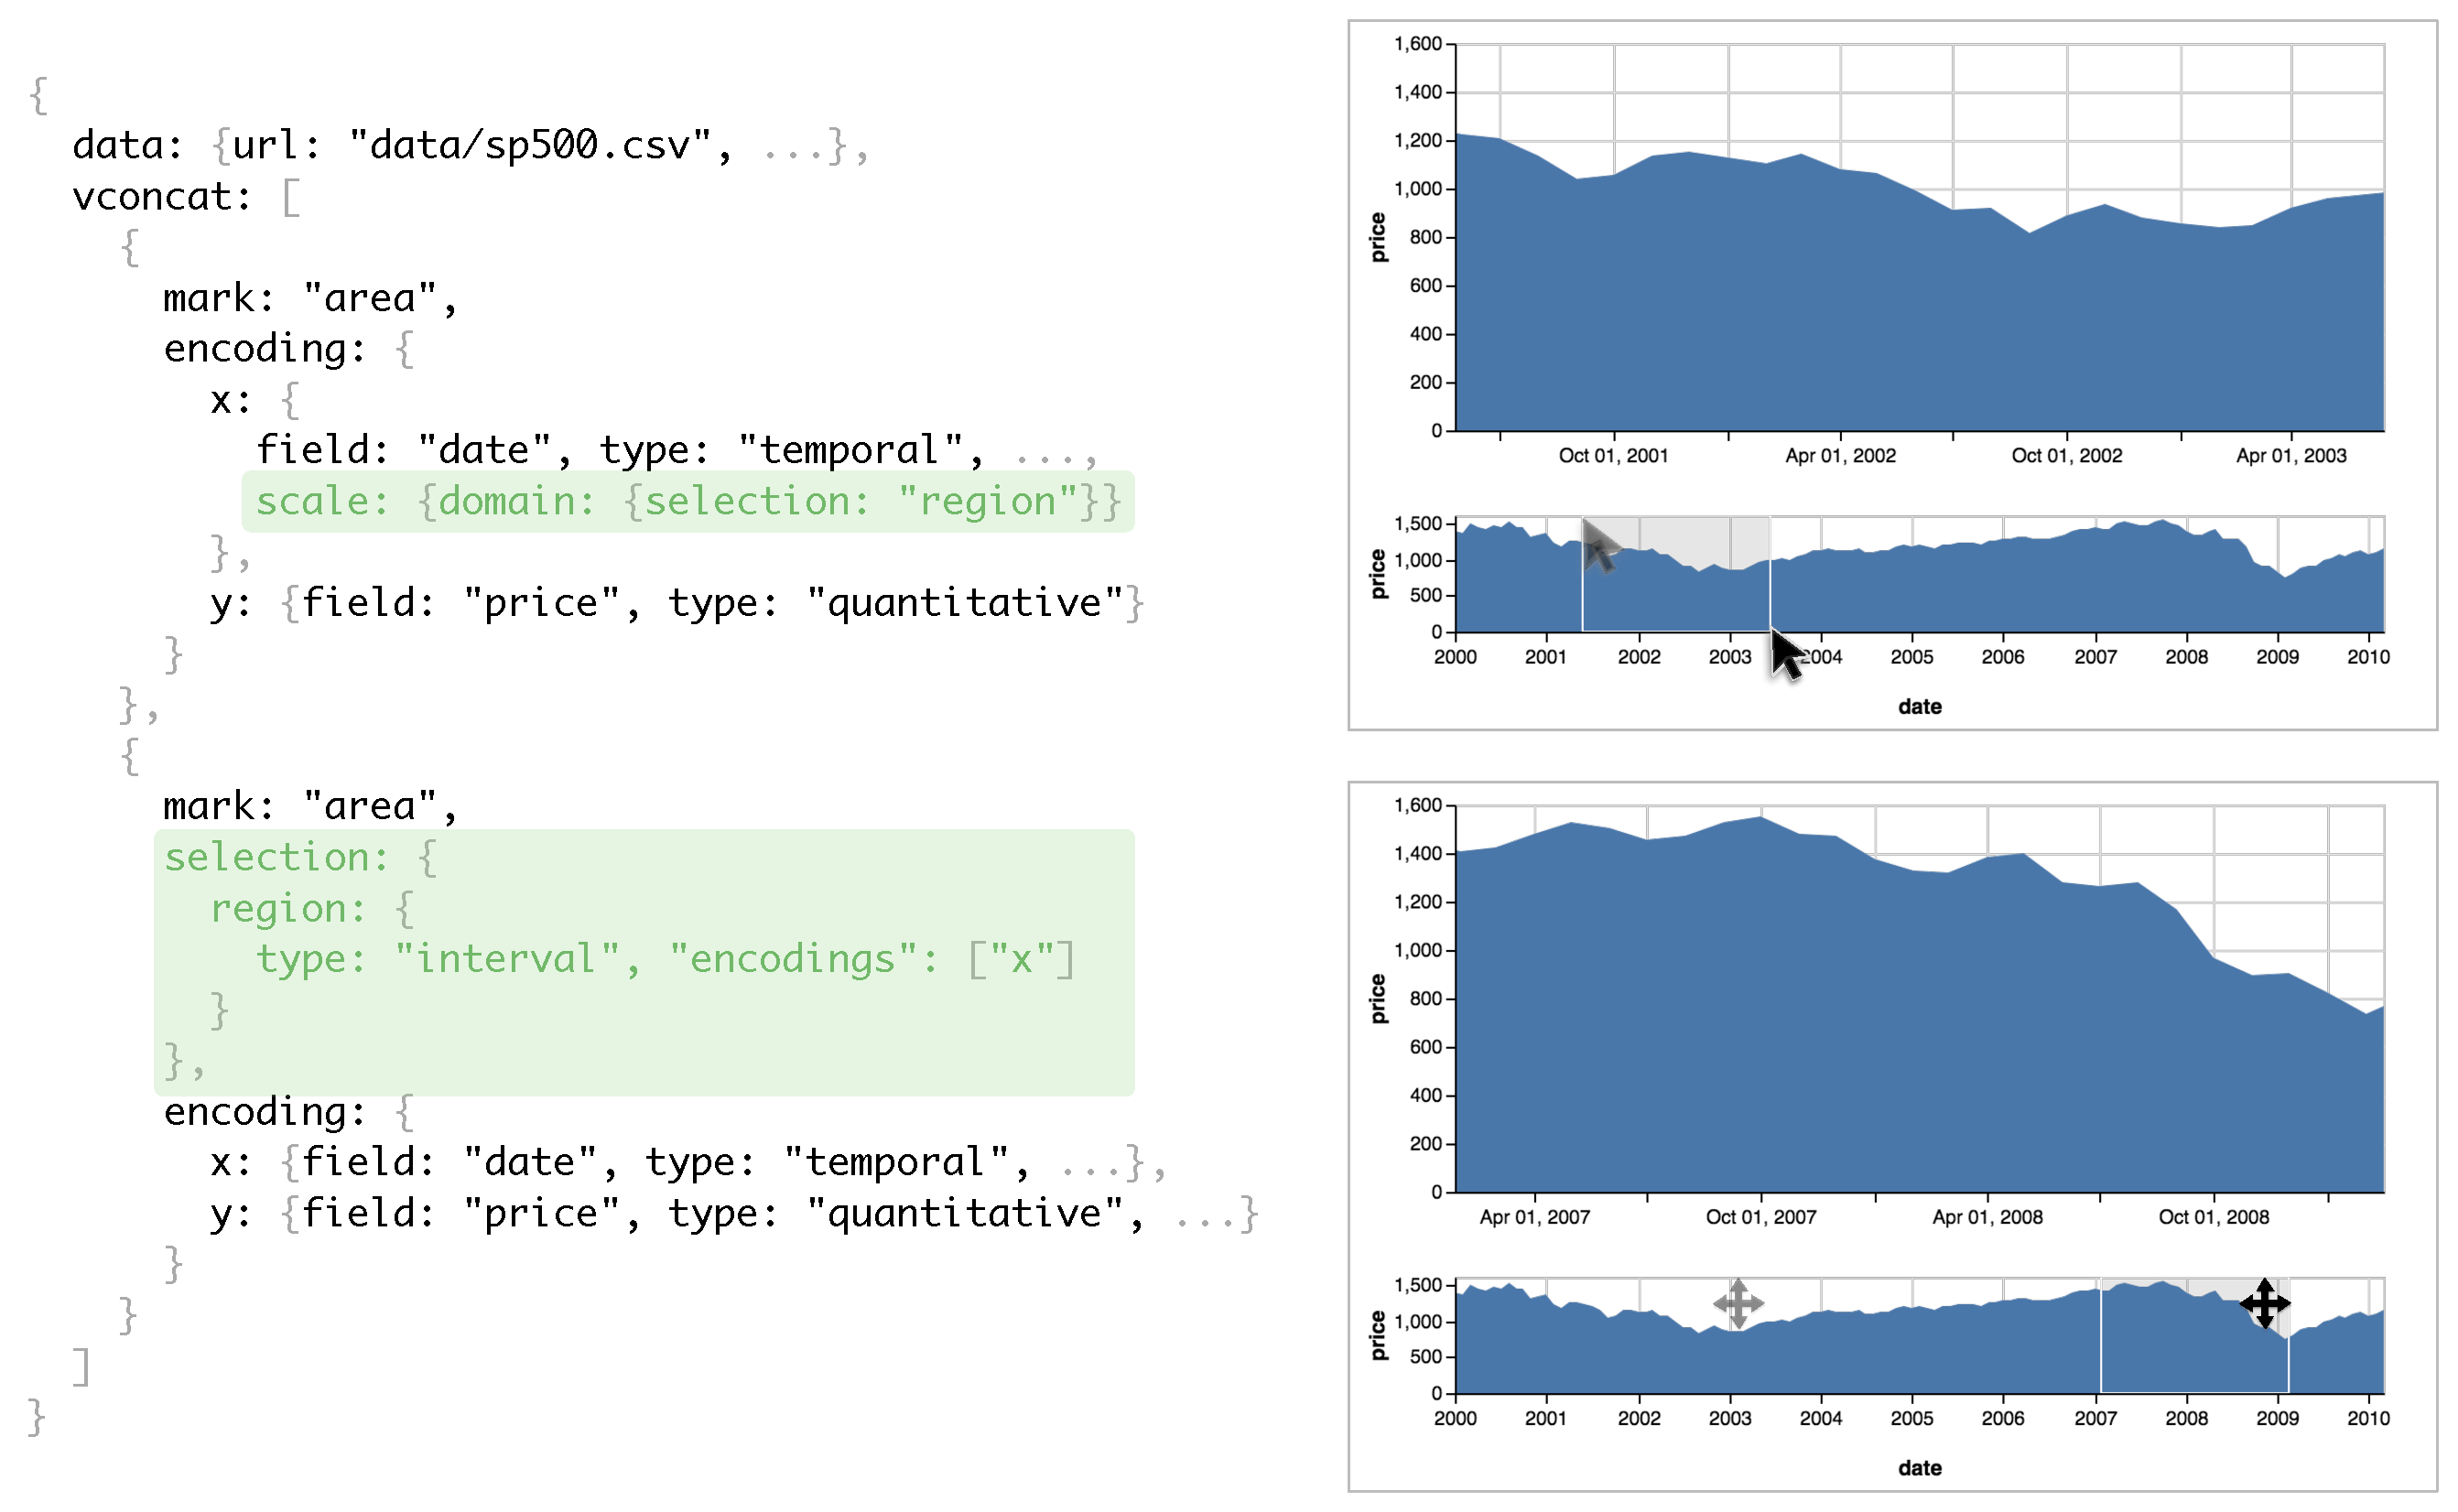
\includegraphics[width=\columnwidth]{overviewDetail}
  \caption{An overview\,+\,detail visualization concatenates two unit
  specifications, with a selection in the second one parameterizing the x-scale
  domain in the first.}
  \label{fig:vl:overviewDetail}
\end{figure}

\subsection{Reconfigure: Index Chart}

\Cref{fig:vl:indexChart} uses a single selection to interactively normalize
stock price time series data as the user moves their mouse across the chart. We
apply the \emph{nearest} transform to accelerate the selection using an
invisible Voronoi diagram. By projecting over the \texttt{date} field, the
selection represents both a single data value as well a set of values that share
the selected \texttt{date}. Thus, we can reference the single selection
directly, to position the red vertical rule, and also materialize it as part of
the \emph{lookup} data transform.

\begin{figure}[h!]
  \centering
  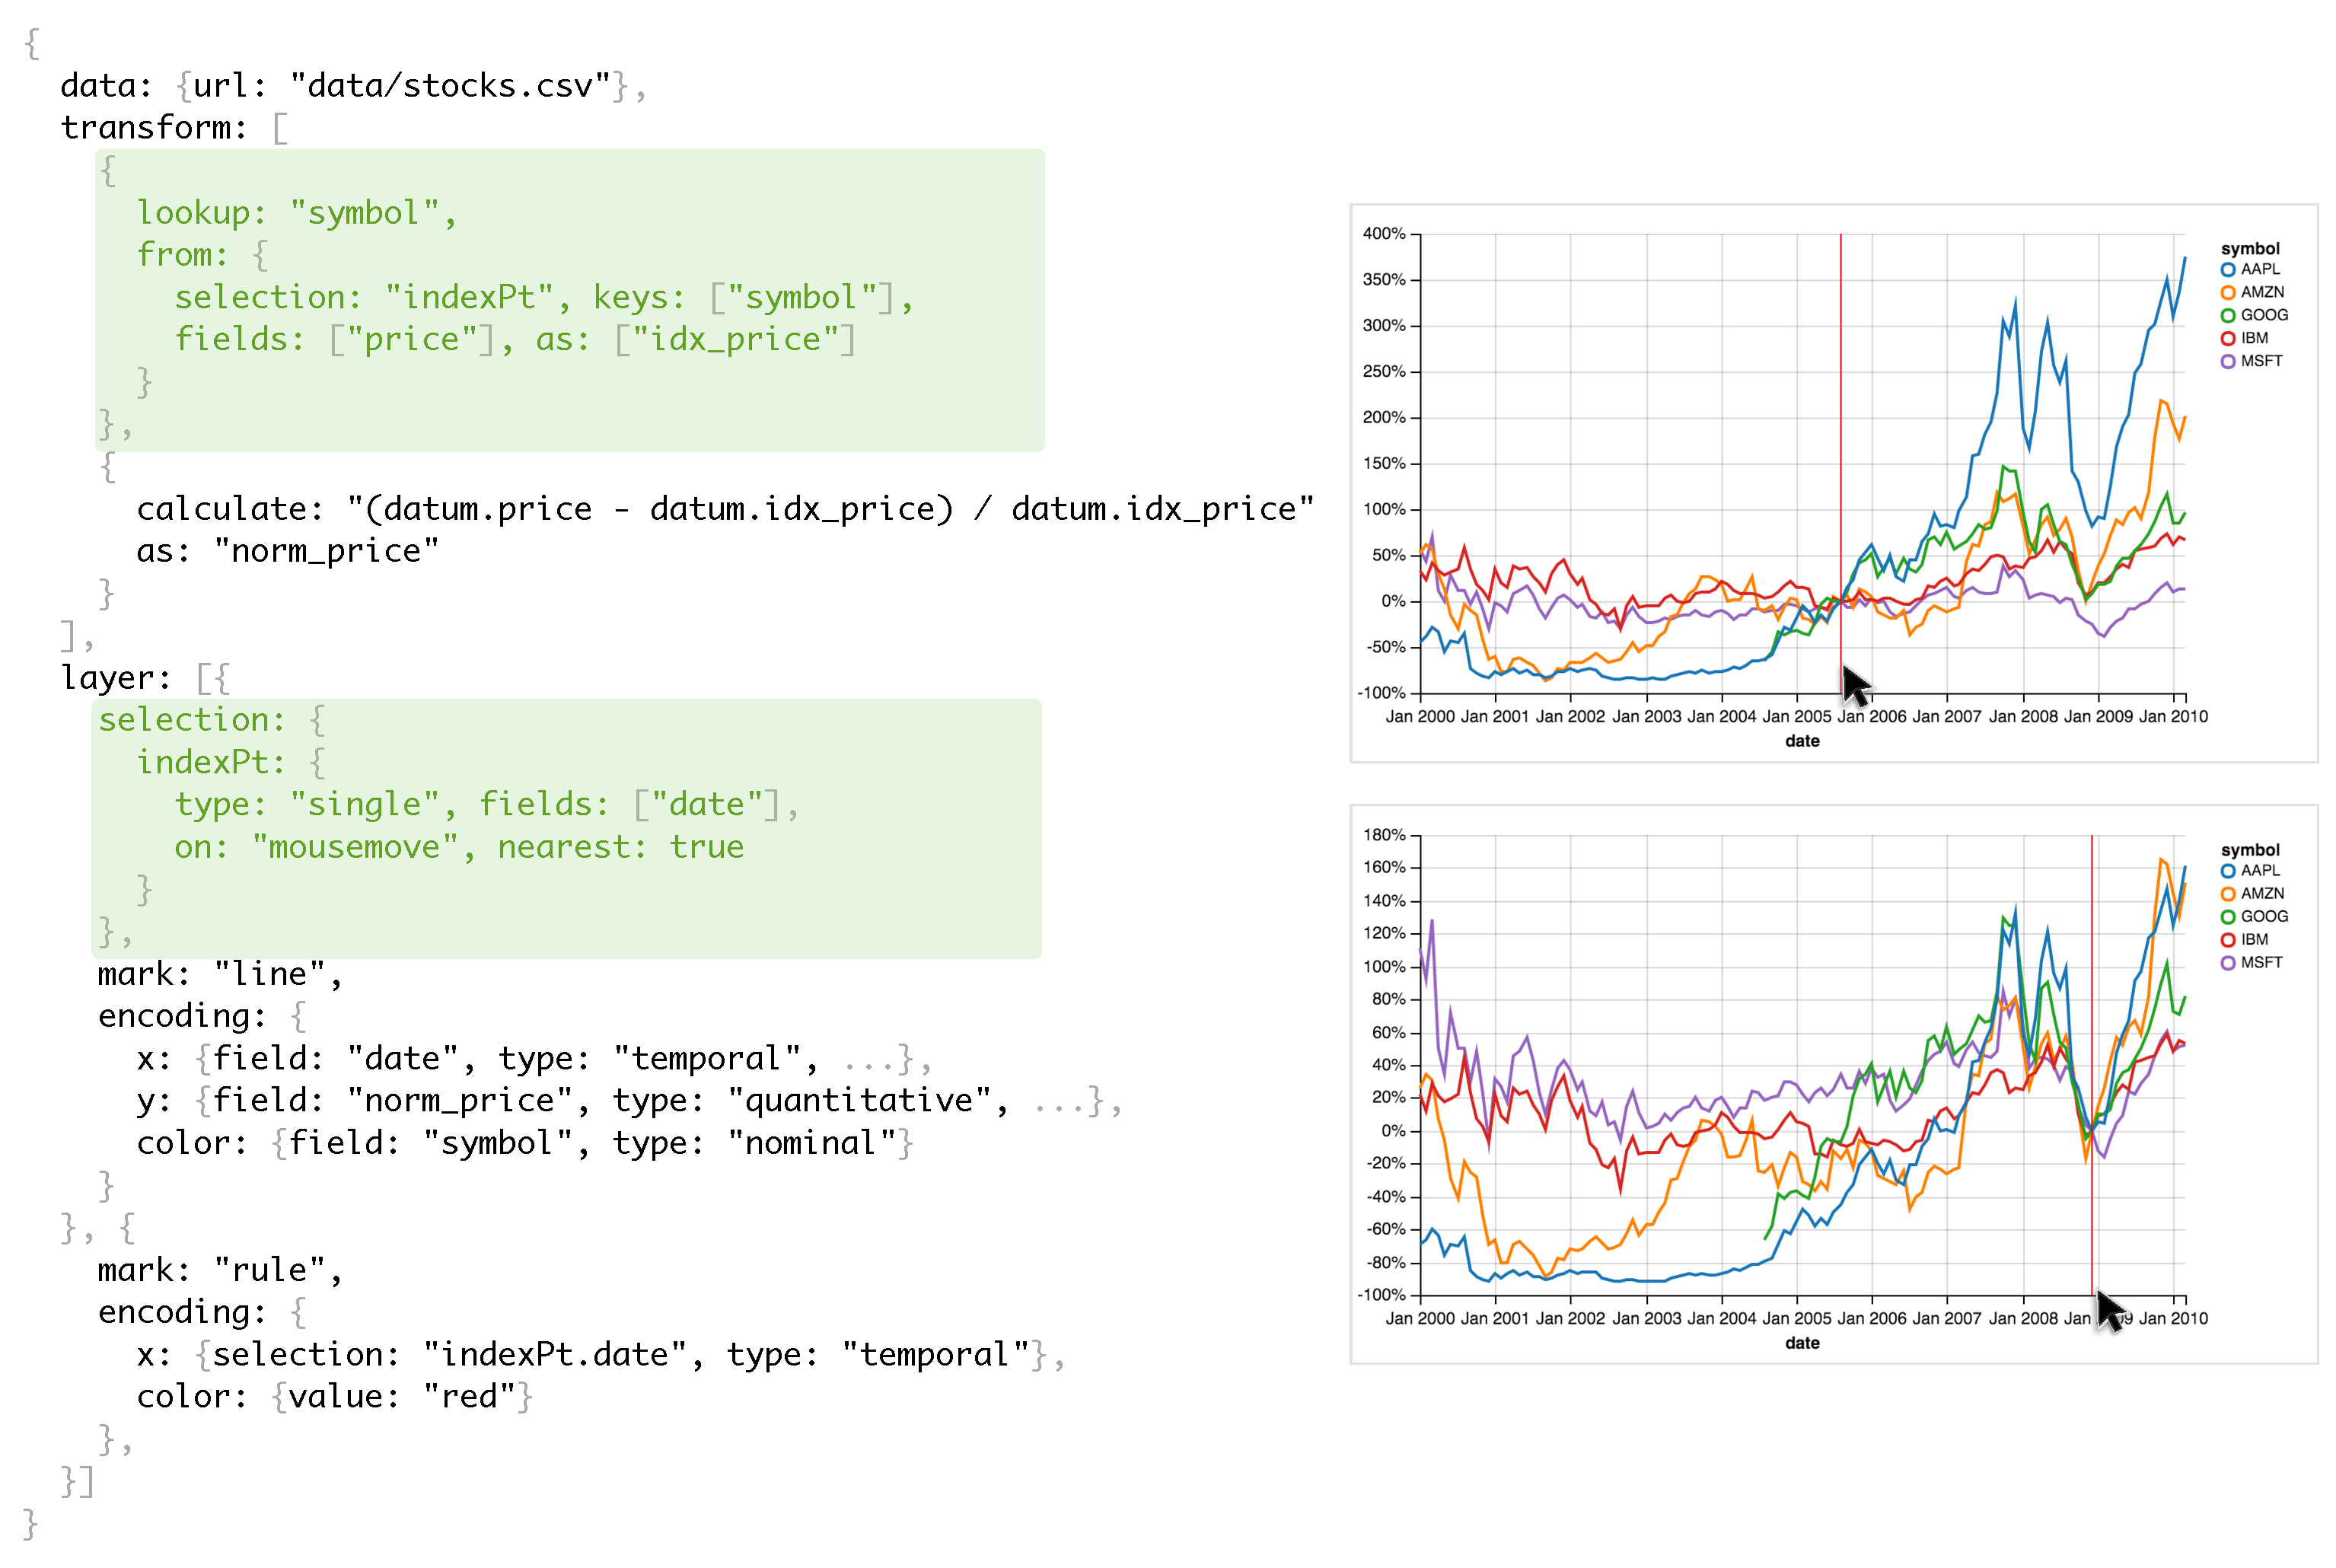
\includegraphics[width=\columnwidth]{indexChart}
  \caption{An index chart uses a single selection to renormalize data based
  on the index point nearest the mouse cursor.}
  \label{fig:vl:indexChart}
\end{figure}

\subsection{Filter: Cross Filtering}

As selections provide a predicate function, it is trivial to use them to filter
a dataset. \Cref{fig:vl:crossfilter}, for example, presents a concise
specification to enable filtering across three distinct binned histograms. It
uses a \emph{repeat} operator with a uni-dimensional interval selection over the
bins set to \emph{intersect others}. The \emph{filter} data transform applies
the selection against the backing datasets such that only data values that fall
within the selection are displayed. Thus, as the user brushes in one histogram,
the datasets that drive each of the other two are filtered, the data values are
re-aggregated, and the bars rise and fall. As with other interval selections,
the Vega-Lite compiler automatically instantiates the \emph{translate}
transform, allowing users to drag brushes around rather than having to reselect
them from scratch.

\begin{figure}[h!]
  \centering
  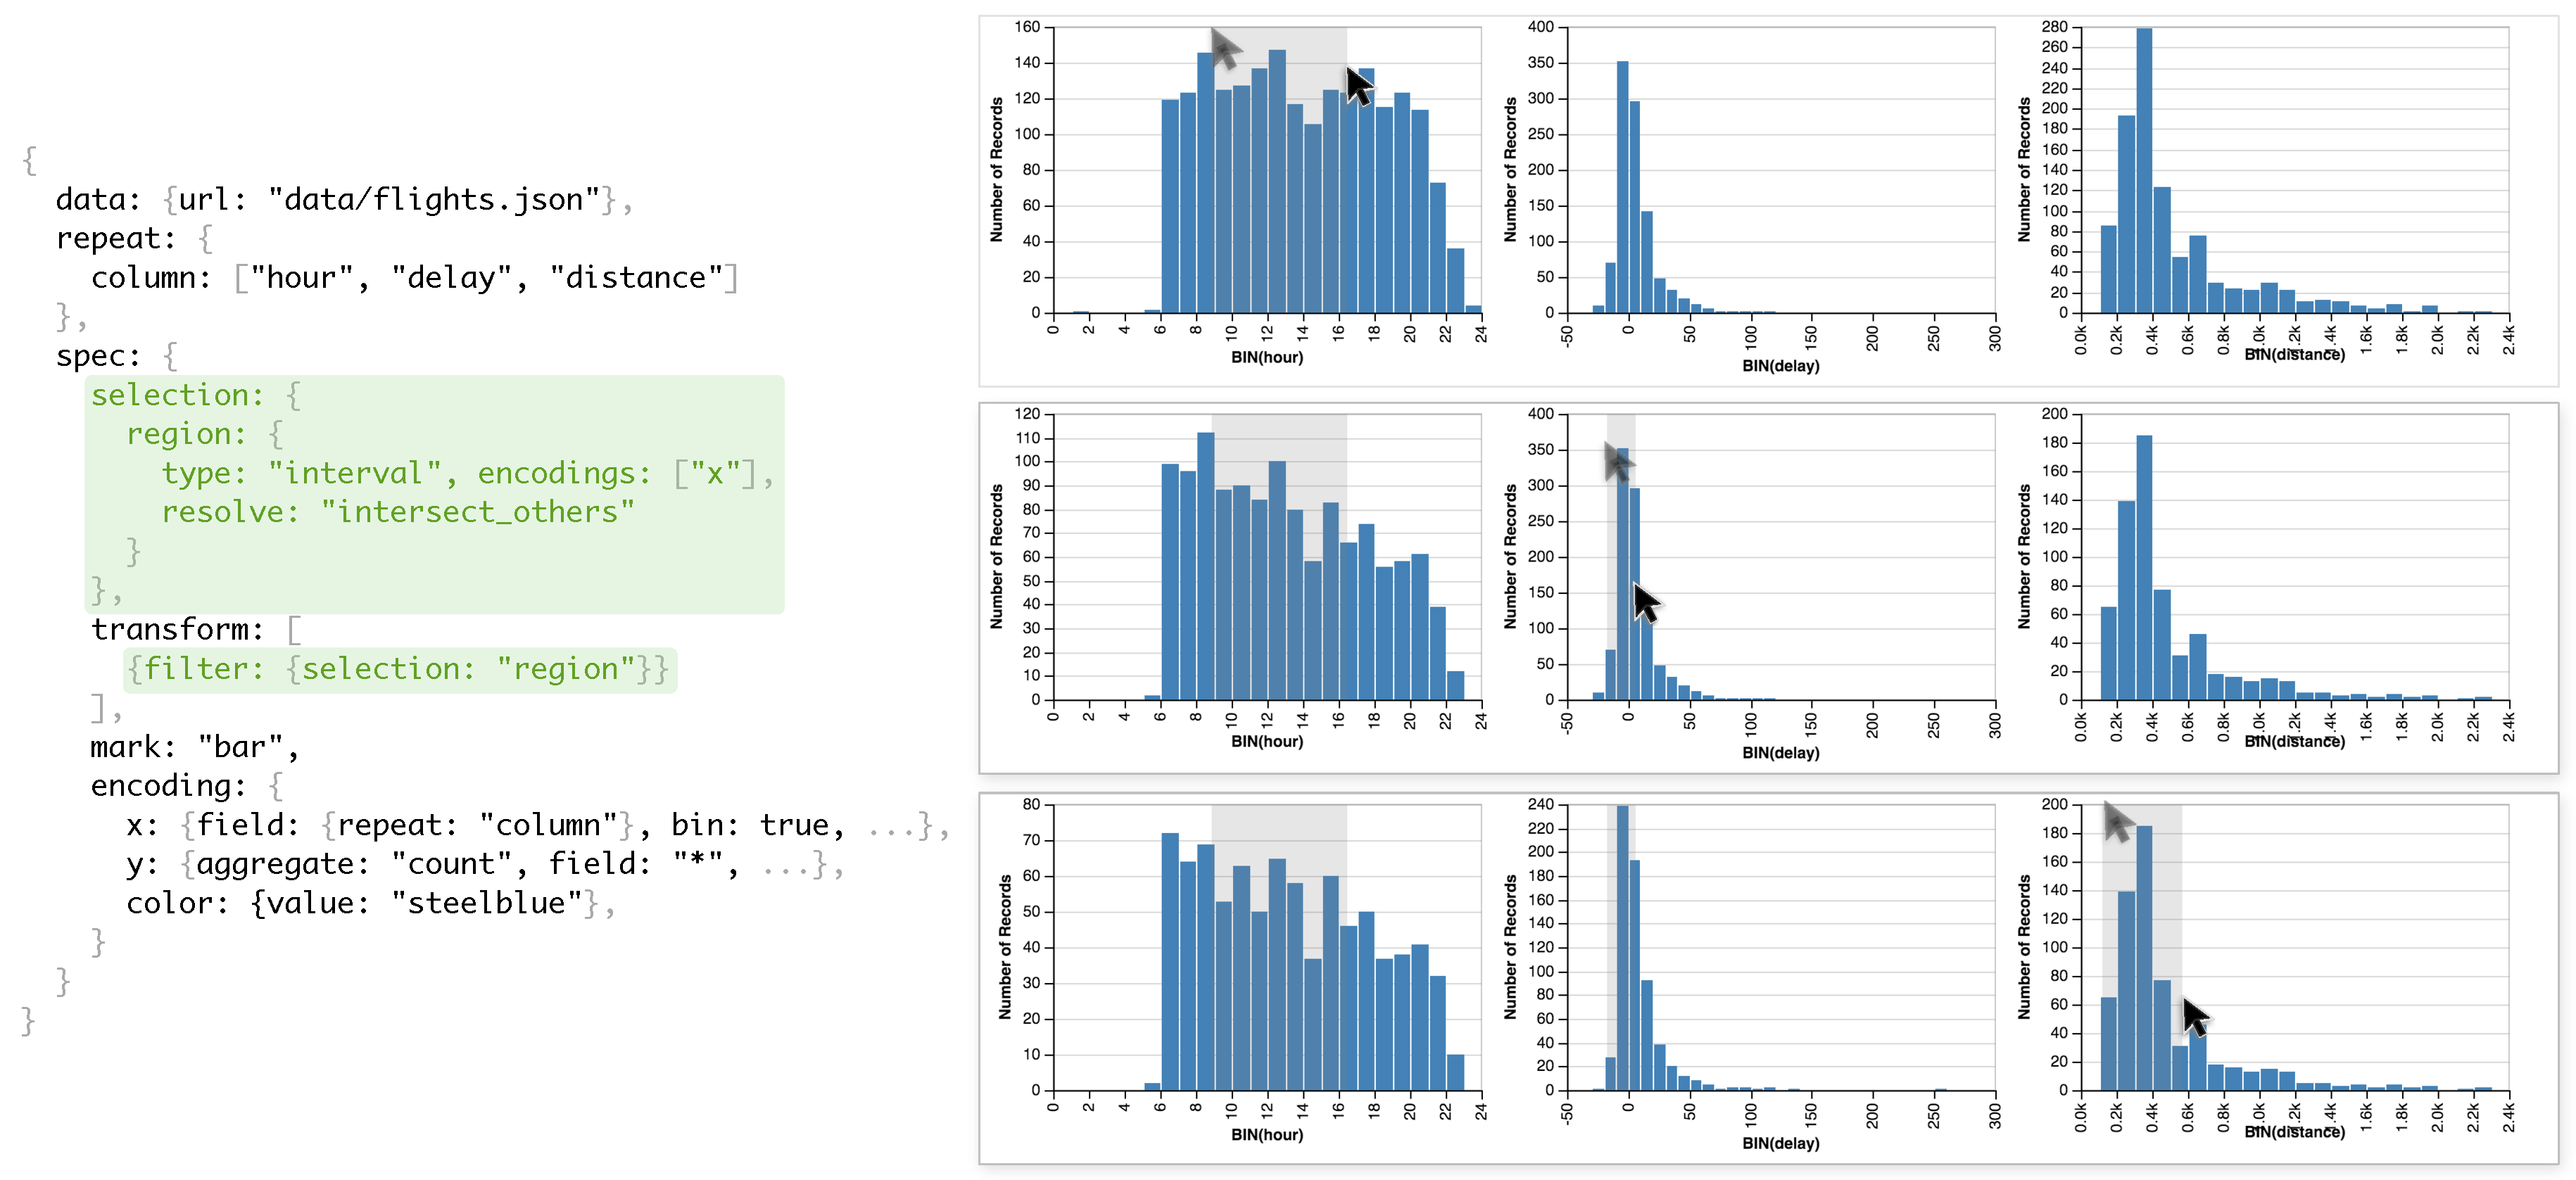
\includegraphics[width=\columnwidth]{crossfilter}
  \caption{An interval selection, resolved to \emph{intersect others}, drives a
  cross filtering interaction. Brushing in one histogram filters and
  reaggregates the data in the others, observable by the varying y-axis labels
  in the screenshots.}
  \label{fig:vl:crossfilter}
\end{figure}

The \emph{filter} data transform can also be used to materialize the selection
as an input dataset for secondary views. For instance, one drawback of
cross-filtering as in \cref{fig:vl:crossfilter} is that users only see the
selected values, and lose the context of the overall dataset. Instead of
applying the selection back onto the input dataset, we can instead materialize
it as an overlay (\cref{fig:vl:layeredCrossfilter}). Now, as the user brushes in
one histogram, bars highlight to visualize the proportion of the overall
distribution that falls within the brushed region(s). With this setup, it is
necessary to change the selection's resolution to simply \emph{intersect}, such
that bars in the brushed plot also highlight during the interaction.

\begin{figure}[h!]
  \centering
  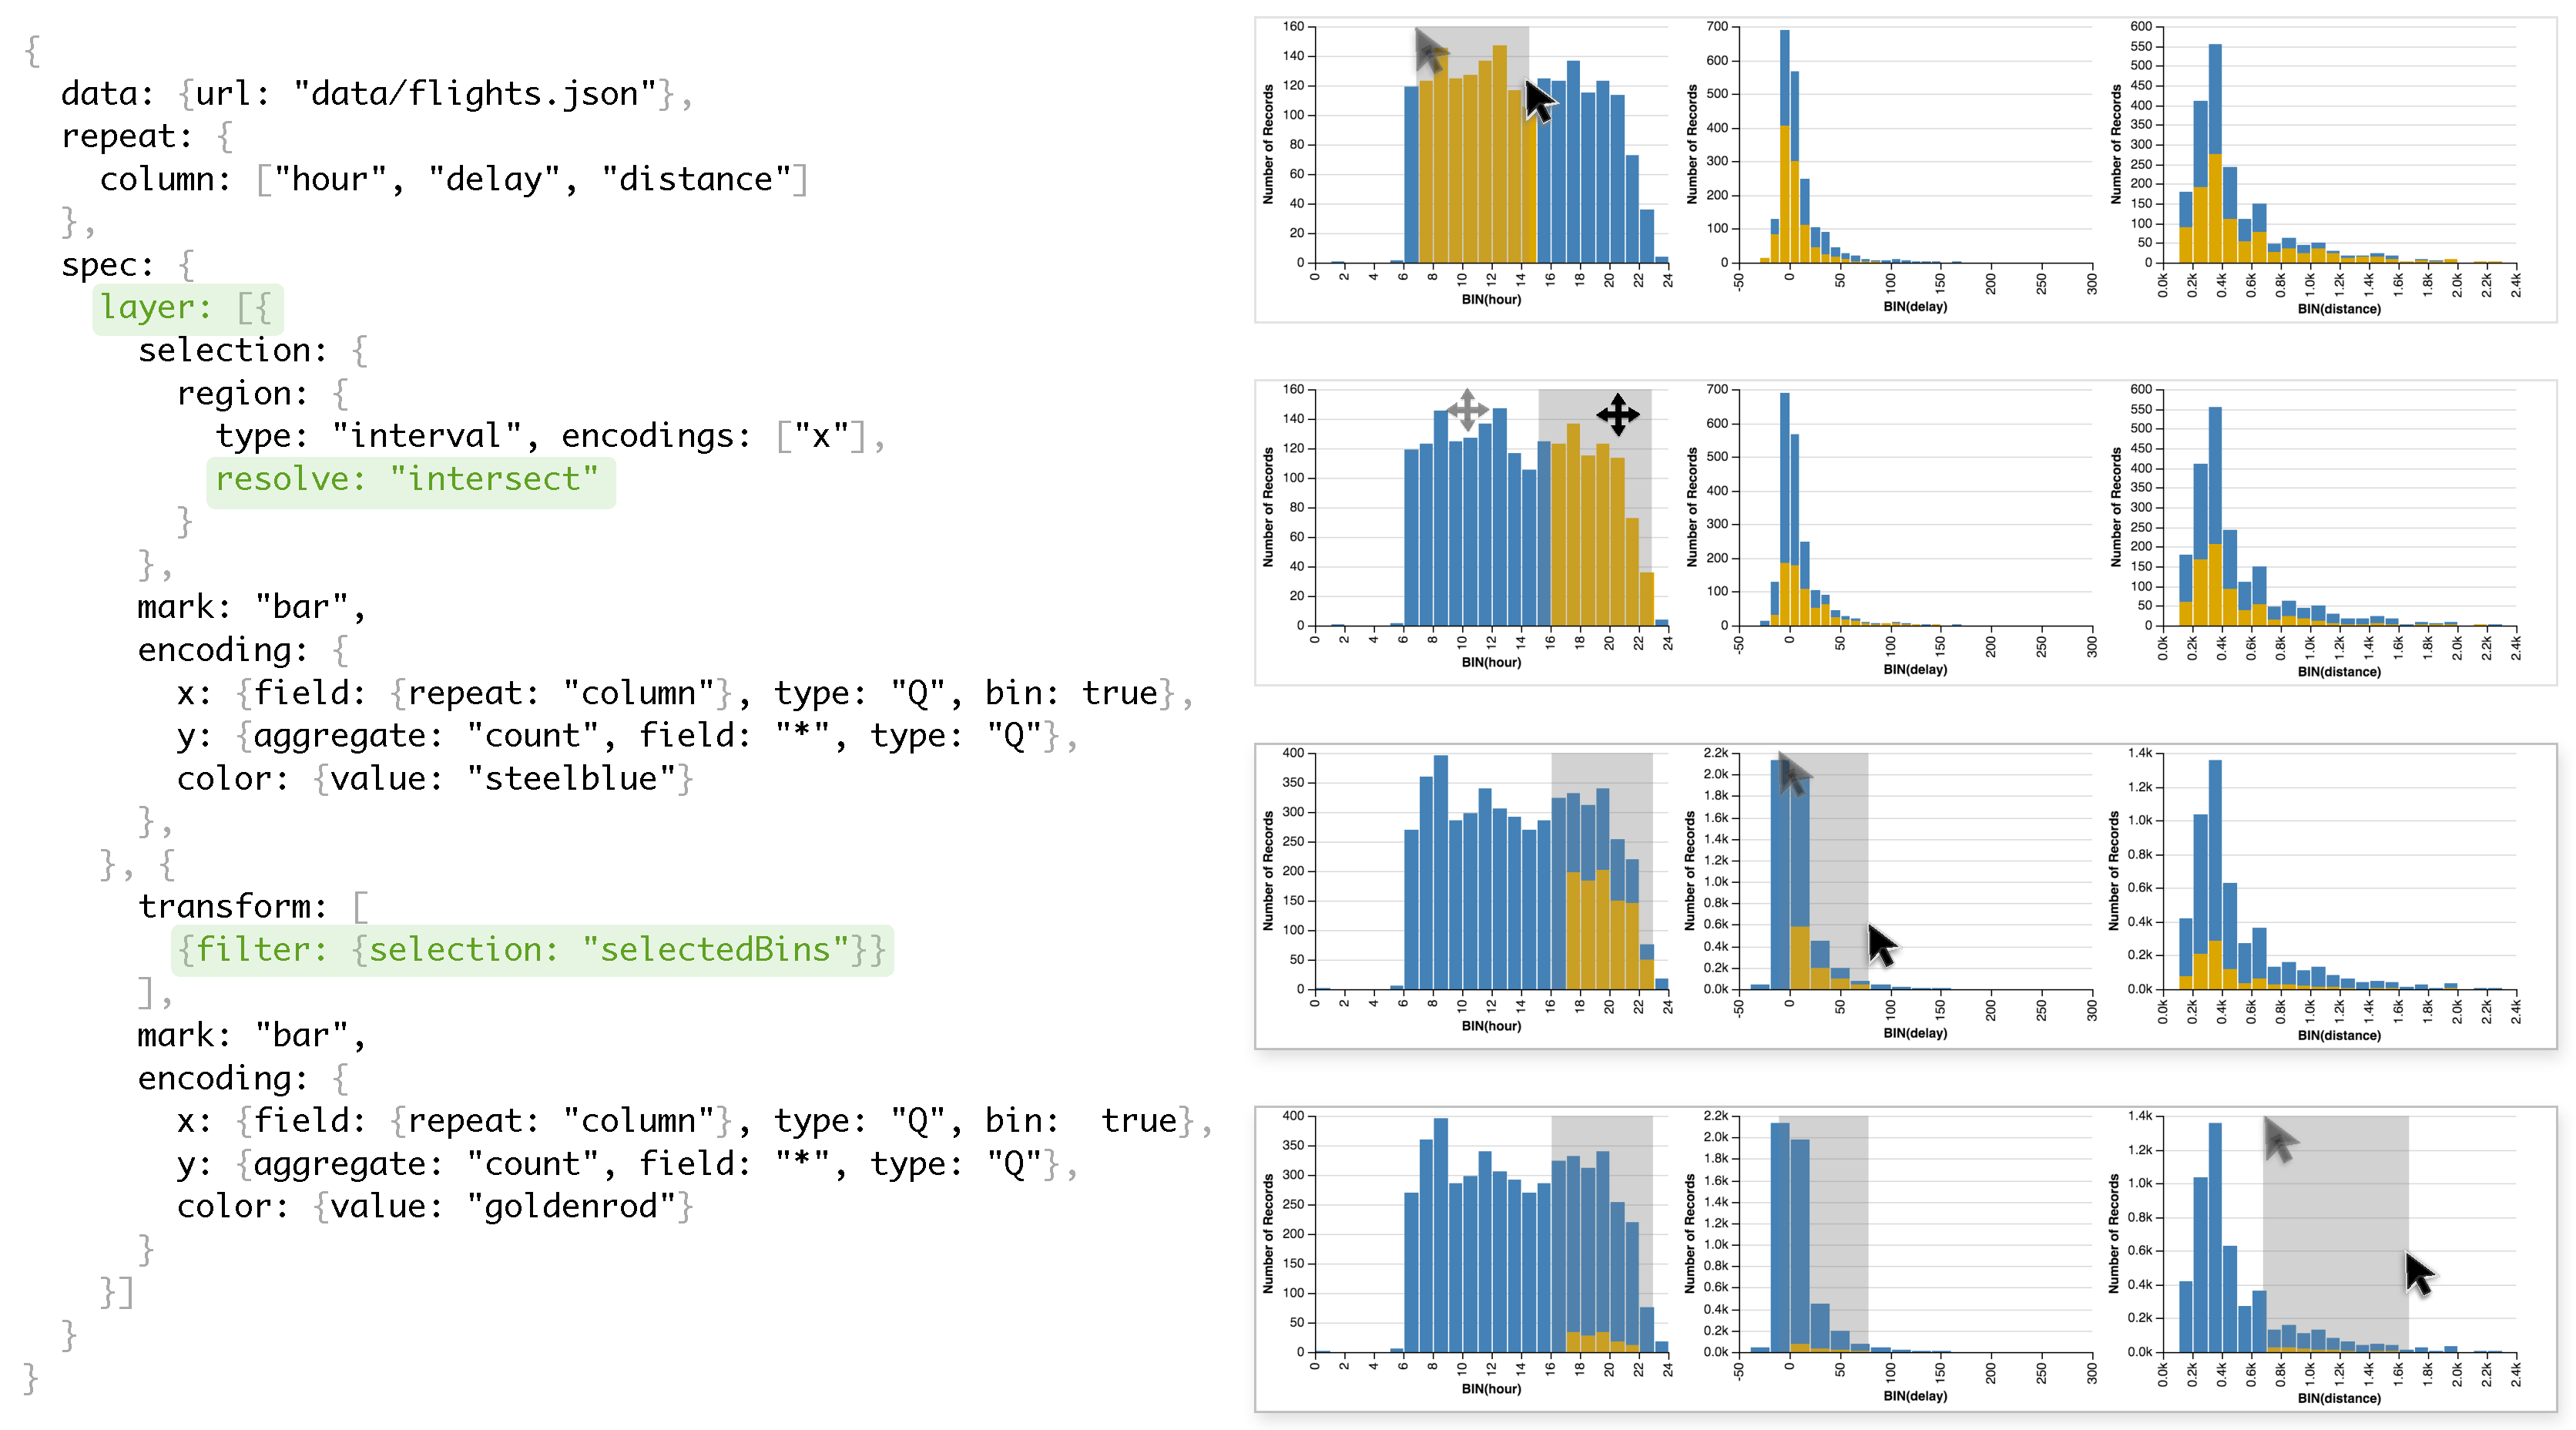
\includegraphics[width=\columnwidth]{layeredCrossfilter}
  \caption{A layered cross filtering interaction is constructed by resolving
  the interval selection to \emph{intersect}, and then materializing it to
  serve as the input data for a second layer. Highlights indicate changes to
  the specification from~\cref{fig:vl:crossfilter}.}
  \label{fig:vl:layeredCrossfilter}
\end{figure}

\subsection{Limitations}

The previous examples demonstrate that Vega-Lite specifications are more concise
than those of the lower-level Vega language, and yet are sufficiently expressive
to cover an interactive visualization taxonomy. Moreover, we have shown how
primitives can be systematically enumerated to facilitate exploration of
alternative designs. Nevertheless, we identify two classes of limitations that
currently exist.

First, there are limitations that are a result of how our formal model has been
reified in the current Vega-Lite implementation. In particular, components that
are determined at compile-time cannot be interactively manipulated. For example,
a selection cannot specify alternate fields to bin or aggregate over. Similarly,
more complex selection types (e.g., lasso selections) cannot be expressed as the
Vega-Lite system does not support arbitrary path marks. Such limitations can be
addressed with future versions of Vega-Lite, or alternate systems that
instantiate its grammar. For example, rather than a \emph{compiler},
interactions could parameterize the entirety of a specification within a
Vega-Lite \emph{interpreter}.

The second class of limitations are inherent to the model itself. As a
higher-level grammar, our model favors conciseness over expressivity. The
available primitives ensure that common methods can be rapidly specified, with
sufficient composition to enable more custom behaviors as well. However, highly
specialized techniques, such as querying time-series data via relaxed
selections~\cite{holz:relaxed}, cannot be expressed by default. Fortunately, our
formulation of selections, which decouple backing points from selected points
via a predicate function, provide a useful abstraction for extending our base
semantics with new, custom transforms. For example, the aforementioned technique
could be encapsulated in a \emph{relax} transform applicable to multi
selections.

While our selection abstraction supports \emph{interactive} linking of marks,
our view algebra does not yet provide means of \emph{visually} linking marks
across views (e.g., as in the Domino system~\cite{gratzl:domino}). Our view
algebra might be extended with support for connecting corresponding marks. For
example, points in repeated dot plots could be visually linked using line
segments to produce a parallel coordinates display.
% !TEX root = ../thesis.tex
\section{Limitations \& Future Work}
\label{sec:vl:conclusion}

The previous section demonstrates that Vega-Lite specifications are more concise
than those of the lower-level Vega language, and yet are sufficiently expressive
to cover an interactive visualization taxonomy. Moreover, we have shown how
primitives can be systematically enumerated to facilitate exploration of
alternative designs. Nevertheless, we identify two classes of limitations that
currently exist.

First, there are limitations that are a result of how our formal model has been
reified in the current Vega-Lite implementation. In particular, components that
are determined at compile-time cannot be interactively manipulated. For example,
a selection cannot specify alternate fields to bin or aggregate over. Similarly,
more complex selection types (e.g., lasso selections) cannot be expressed as the
Vega-Lite system does not support arbitrary path marks. Such limitations can be
addressed with future versions of Vega-Lite, or alternate systems that
instantiate its grammar. For example, rather than a \emph{compiler},
interactions could parameterize the entirety of a specification within a
Vega-Lite \emph{interpreter}.

The second class of limitations are inherent to the model itself. As a
higher-level grammar, our model favors conciseness over expressivity. The
available primitives ensure that common methods can be rapidly specified, with
sufficient composition to enable more custom behaviors as well. However, highly
specialized techniques, such as querying time-series data via relaxed
selections~\cite{holz:relaxed}, cannot be expressed by default. Fortunately, our
formulation of selections, which decouple backing points from selected points
via a predicate function, provide a useful abstraction for extending our base
semantics with new, custom transforms. For example, the aforementioned technique
could be encapsulated in a \emph{relax} transform applicable to list selections.

While our selection abstraction supports \emph{interactive} linking of marks,
our view algebra does not yet provide means of \emph{visually} linking marks
across views (e.g., as in the Domino system~\cite{gratzl:domino}). Our view
algebra might be extended with support for connecting corresponding marks. For
example, points in repeated dot plots could be visually linked using line
segments to produce a parallel coordinates display.

An early version of Vega-Lite is used to automatically recommend static plots as
part of the Voyager browser~\cite{voyager}. Voyager leverages perceptual
\emph{effectiveness criteria}~\cite{bertin:semiology, cleveland:perception,
mackinlay:apt} to rank candidate visual encodings. One promising avenue for
future work is to develop models and techniques to analogously recommend
suitable interaction methods for given visualizations and underlying data types.
Here, the human-computer interaction literature~\cite{beaudouin:instrumental}
may offer insights on when and why users benefit from certain interaction
techniques.

Vega-Lite is an open source system available at
\url{http://vega.github.io/vega-lite/}. By offering a multi-view grammar of
graphics tightly integrated with a grammar of interaction, Vega-Lite facilitates
rapid exploration of design variations. Ultimately, we hope that it enables
analysts to produce and modify interactive graphics with the same ease with
which they currently construct static plots.
% !TEX root = ./thesis.tex
\graphicspath{{./figures/lyra/}}
\chapter{An Interactive Visualization Design Environment (VDE)}

\bibliographystyle{plain}
\bibliography{thesis}
\end{document}